\clearpage
\section{Deep Learning Background}\label{Sec:Deep_Learning_Background}


\textbf{What is Deep Learning?} \textit{ Deep Learning is a new approach to Machine Learning research which focuses on learning and understanding from the data without the need for a human operator to formally specify all the knowledge that the computer needs. This method is built using a hierarchy of concepts which enables the computer to learn complex concepts by building them layer by layer from simpler ones. A graph which shows how this concept is built will permit us to figure out a very deep graph with many layers; for this reason, we call this approach to AI deep learning~\cite{Goodfellow-et-al-2016}}.\\

There were many early trials to utilize the AI in real life problems. For example, IBM's Deep Blue chess-playing system which defeated world champion Garry Kasprov in 1997 (Hsu, 2002).\\ %@@@@MUST add the reference

Another approach to AI used hard-code knowledge about the world in informal language. A computer can understand statements from the formal language automatically using logical inference rules. This is known as the knowledge base approach to artificial intelligence rules. None of these projects has achieved significant success. For Example, Cyc has tried to gather a comprehensive ontology and knowledge base about the basic concepts of how the world works (Lenat and Guha, 1989).%@@@@MUST add the reference
Cyc is an inference engine and a database of statements in a language called Cycl. A staff of human supervisors enters these statements. People struggle to devise formal rules with sufficient complexity to describe the world accurately~\cite{Goodfellow-et-al-2016}.\\

The difficulty faced in the previous system is because the hard-coded knowledge has shown up the AI need to acquire its knowledge from the data itself. This capability is known as machine learning. This approach has introduced some algorithms which solve and tackle the problems from which we can, for example, check if the email is spam or not. Also, it is used for other problems, such as price predictions for housing. An example of these algorithms is \textit{Naive Bayes} and \textit{Logistic regression}.

This simple machine learning approach is working in the data but not with its original format; it requires some different representation to be input to the model. This different representation is named feature engineering. In the of Feature Engineering deciding whether email is spam or not, it can be word frequency, char frequency, class attributes, capital letters frequency, or some other data processing such as removing stop words from the input lemmatization. So, all the previous features provided by a human expert (who knows the problem in detail and analyzes which of its features affect the data) are then added as a feature to the input model.
   

However, for many tasks, it is difficult to identify the features which should be extracted. For example, we need to detect cars in photographs. We know every car has wheels. So, to detect cars, we can check if there is a wheel to be a feature for car detection. However, to detect or to describe wheels in terms of pixel values is a difficult task. The image may not be clear or may be complicated by shadows, the sun glaring off the metal parts of the wheel, the blurring in images may sometimes make it unclear, and so on~\cite{Goodfellow-et-al-2016}. One solution to this problem is to use machine learning itself to discover not only the output of the model but also the features which are the input for the model. This approach is known as representation learning. Learned representation can achieve better results than hard-designed representation. This approach also allows AI systems to rapidly adapt to new tasks or be automatically identified from any new data. Representation learning can automatically discover many features quickly or can take more time in case of complex tasks, but will at least provide an excellent set of features which can be adapted for any complex problem without the need for manual features. In this research, we used the AI to identify the features for our model, enabling this model to achieve breakthrough results, compared with the old method of manual feature machine learning.

If we go back to the image example, we can show that it is not an easy task to extract features to detect the car from an image. So, Deep Learning is trying to solve this problem in feature engineering by introducing representation learning that build complex representations in terms of another simpler layer of representations. Figure~\ref{Fig:Deep_Learning_Image_Person_Example} shows how deep learning represents an image of a person by combining simpler representation, e.g. the edges and contours which led to understanding complex representations. The benefit from allowing the computer to understand the data and building the representation is the ability to build and understand very complex representation and also to utilize and combine features from simpler to deep representations with many ways such as recurrence or sequences.
\begin{figure}[!ht] 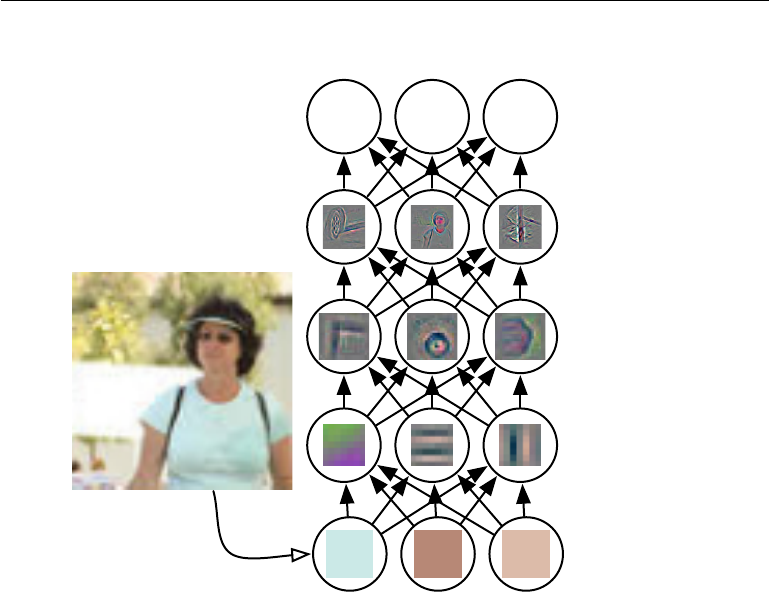
\includegraphics[width=\linewidth]{./Figures/Ch_2_Background/DeepLearningImagePersonExample.png}
	\caption{Illustrations on how Deep Learning can work based on images figure presented~\cite{Goodfellow-et-al-2016}~\cite{Zeiler2014}.}
	\label{Fig:Deep_Learning_Image_Person_Example}
\end{figure}

{\color{red}

Another example is using DL in text generation problems. Lots of research works to use DL to generate text after learning the pattern from the text for example, train the model on Shakespeare’s poems and then the model try to generate a similar text. We can also use DL to classify the text similar idea of our research work. The main idea is how to use these techniques to get best results without hand-crafted feature engineering.

}

Modern deep learning provides a compelling framework for learning data problems. This model becomes more complex by the adding more layers and more units within a layer. The Deep Learning model works perfectly on the big dataset which allows the model to learn the data features in a good way.

In the remaining parts in this section we start introducing the main concepts and components used in deep learning, and the basic units of Recurrent Neural networks and LSTM.%

\subsection{Logistic Regression}


Logistic Regression is a machine learning algorithm which we can assume has the basic idea behind the deep learning (explained later). Logistic Regression is also one of the most used machine learning techniques for binary classification.

A simple example of logistic regression would be an algorithm for fraud detection. It takes some raw data input and detects if it is a fraud case or not. Assume fraud case is one and non-fraud case is zero. David Cox developed logistic regression in 1958~\cite{Cox2958}. The “logistic” name came from its core logistic function, also named \textit{Sigmoid function} function in Equation~\eqref{eq:logistic_function}. The Logistic function is shaped as an S-shape.

One of these function features can take any input real number and convert it into a value between 1 and 0.%
\begin{figure}
\centering
\begin{tikzpicture}
  \begin{axis}%[
%grid=major,
xmin=-10,
xmax=10,
axis x line=bottom,
ytick={0,.5,1},
%xticklabels = {,,}, 
ymax=1,
axis y line=middle,
]
\addplot%
[
blue,%
mark=none,
samples=100,
domain=-10:10,
]
(x,{1/(1+exp(-x))});

%(x,{x^2});
\end{axis}

\end{tikzpicture}%
\caption{Logistic Regression Function (S-Shape)}\label{Fig:Logistic}
\end{figure}%

Example: given x, we want to get the predictions of $\widehat{y}$ which is the estimate of $y$ when $\widehat{y}$ is presented in Equation~\eqref{eq:yhat_estimate}. So, to calculate the output function for Logistic Regression using Equation~\eqref{eq:logistic_regression_yhat}. Note: if we remove the Sigmoid function $\sigma$ from the equation it becomes the Linear Regression model and $\widehat{y}$ can be greater than 1 or negative. Figure~\ref{Fig:Logistic} shows the Sigmoid function output.%
\begin{equation}\label{eq:logistic_function}
 x = \frac{1}{1-e^{-x}} \quad \text{where} \quad x \in \mathbb{R}^{n_x} 
\end{equation}
\begin{equation}
 \label{eq:yhat_estimate}
  \widehat{y} = P(y=1 | x) \quad \text{where} \quad 0 \le \widehat{y} \le 1
 \end{equation}
\begin{equation}
 \label{eq:logistic_regression_yhat}
 \widehat{y} = \sigma(w^t x + b) \quad \text{where:} \quad \sigma(z) = \frac{1}{1-e^{-z}} \text{, } w \in \mathbb{R}^{n_x} \text{, } b \in \mathbb{R} 
\end{equation}%
%
\subsubsection{Loss Error Function}
Loss Error Function is the function which describes how well our algorithm can understand $\widehat{y}$ y b when the true label is y. It also can be defined as the difference between the true value of $y$ and the estimated value of $\widehat{y}$.~\footnote{\textit{Parts of this subsections are explained into Andrew NG Coursera courses in deep learning and written using our understanding of this topic but the equations and the idea is taken from the course}}. Equation~\eqref{eq:loss_function} describe the loss function for Logistic Regression. There are other functions which can represent the loss functions but we take the example below. As we know $y$ is the label which should be 1 or 0, this function makes sense to describe the loss function is outlined below:%
\begin{itemize}
\item in case (y = 1) Equation~\eqref{eq:loss_function} we need $\widehat{y}$ to be as big as possible to be equal or near \textit{y true}, which is 1. So, $ - (\log \widehat{y} )$ will provide the value. Note, as explained before, Sigmoid function can't be greater than 1 or less than 0. 
\item in case (y = 0) Equation~\eqref{eq:loss_function} we need $\widehat{y}$ to be as small as possible to be equal or near \textit{y true}, which is 0. So, $- \log (1-\widehat{y})$ will provide the value. 
\end{itemize}%
%
\begin{equation}
 \label{eq:loss_function}
  \ell(y,\widehat{y}) = - (y \log \widehat{y} + (1-y) \log (1-\widehat{y})) =  \begin{cases}
- (1\times \log \widehat{y} + (1-1) \log (1-\widehat{y})) = - (\log \widehat{y} ) & \mbox{if }  y = 1\\
- (0\times \log \widehat{y} + (1-0) \log (1-\widehat{y})) = - \log (1-\widehat{y}) & \mbox{if } y = 0
\end{cases}
\end{equation}%
%
%\begin{equation} \label{eq:loss_function_log_y_1}
%\begin{split}
% \text{(if y = 1) } \quad \ell(y,\widehat{y}) & = - (y \log \widehat{y} + (1-y) \log (1-\widehat{y})) \\
% & = - (1 \log \widehat{y} + (1-1) \log (1-\widehat{y}))\\
% & = - (\log \widehat{y} )
%\end{split}
%\end{equation}
%\begin{equation} \label{eq:loss_function_log_y_0}
%\begin{split}
% \text{(if y = 0) } \quad \ell(y,\widehat{y}) & = - (y \log \widehat{y} + (1-y) \log (1-\widehat{y})) \\
% & = - (0 \times \log \widehat{y} + (1-0) \log (1-\widehat{y}))\\
% & = - \log (1-\widehat{y})
%\end{split}
%\end{equation}
%
\subsubsection{Cost Function}
To predict $y$ from $\widehat{y}$, we learn from the input parameters in this case it will be \textbf{\textit{(w,b)}} from Equation~\eqref{eq:logistic_regression_yhat} as \textbf{\textit{(w,b)}} are the parameters which define the relation between input dataset X and the output Y. So, Cost Function will measure how well you are doing in an entire training set and the ability to understand the relation between X,Y.

Cost function \textbf{\textit{$J$}} in Equation~\eqref{eq:cost_function} is the average of loss function applied to every training example which equals the sum of the loss for each training example divided by the total number of training examples%
%
\begin{equation}\label{eq:cost_function}
 \begin{split}
 J(w,b) & = \frac{\sum_{i=1}^{m} \ell(y^i,\widehat{y^i})}{m} \quad \text{ where m is the total number of training example} \\
 & = \frac {- \sum_{i=1}^{m} [(y^i \log \widehat{y^i} + (1-y^i) \log (1-\widehat{y^i}))]}{m} 
 \end{split}
\end{equation}%
%
\subsubsection{Convex Function vs Non-Convex Function }

In this subsection we give an overview of the convex and non-convex functions and their relation with deep learning. We do not explain the proofs or write them. We explain in general the definition and its related features to our topic.

\begin{description}
 \item [\textbf{Convex Function}]: In mathematics, a real-valued function defined on an n-dimensional interval is called \textit{convex} if the line segment between any two points on the graph of the function lies above or on the graph, in a Euclidean space (or more generally a vector space) of at least two dimensions~\cite{Wiki_Convex_Function}. More generally, a function $f(x)$ Figure~\ref{Fig:Convex_Function} is \textit{convex} on an interval $[a,b]$ if for any two points $x_1$ and $x_2$ in $[a,b]$ and any $\lambda$ where $0<\lambda<1$~\cite{Rudin_1976},%
%
\begin{equation}\label{eq:convex_fun}
 f(\lambda x_1 + (1-\lambda)x_2) \leq \lambda f(x_1) + (1 - \lambda) f(x_2)
\end{equation}%
%
For a twice differentiable function of a single variable, if the second derivative is always greater than or equal to zero for its entire domain then the function is \textit{convex}. Well-known examples of convex functions include the quadratic function $X^2$ Figure~\ref{Fig:Derivative_Example}. So, If $f(x)$ has a second derivative in $[a,b]$, then a necessary and sufficient condition for it to be \textit{convex} on that interval is that the second derivative $f^{''}(x) \geq 0$ for all $x$ in $[a,b]$~\cite{Wolfram_Convex}.

If the inequality above is strict for all $x_1$ and $x_2$, then $f(x)$ is called \textbf{strictly convex}. \textit{Convex function} on an open set has no more than one minimum. So, in strictly convex, the local minimum = global minimum. This feature is very important for any optimization problem. As we can see, most of deep learning problems are related to how to optimize the function to find the minimum point in this function.  It is an easy problem to face a convex function but in the real world most cases are non-convex functions.

\item [\textbf{Non-Convex Function}]: In mathematics, a Non-Convex (also named concave) function is the negative of a \textit{convex function}. A function $f(x)$ is said to be concave on an interval $[a,b]$ if, for any points $x_1$ and $x_2$ in $[a,b]$, the function $-f(x)$ is convex on that interval.%
\begin{equation}\label{eq:concave_fun}
 \begin{split}
f(\lambda x_1 + (1-\lambda)x_2) \geq \lambda f(x_1) + (1 - \lambda) f(x_2)
 \end{split}
\end{equation}%
The function is also called strictly concave if,
\begin{equation}\label{eq:concave_fun_strictly}
 \begin{split}
f(\lambda x_1 + (1-\lambda)x_2) > \lambda f(x_1) + (1 - \lambda) f(x_2)
 \end{split}
\end{equation}%
%
If $f$ is twice-differentiable, then $f$ is concave if and only if $f^{''}$ is non-positive (or, informally, if the "acceleration" is non-positive). If its second derivative is negative then it is strictly concave, but the opposite is not true, as shown by $f(x) = −x^4$~\cite{Wiki_Concave_Function}. Also, a differentiable function $f$ is (strictly) concave on an interval if and only if its derivative function $f^`$ is (strictly) monotonically decreasing on that interval; that is, a concave function has a non-increasing (decreasing) slope. The problem for non-convex optimization is to find the local minimum. Sometimes many local minimums  can be found and it may be hard to optimize this function Figure~\ref{Fig:Concave_Function}.%
\end{description}
%
\begin{figure}[t]
 \centering
 \subfigure[Convex Function Example]{~\label{Fig:Convex_Function}
 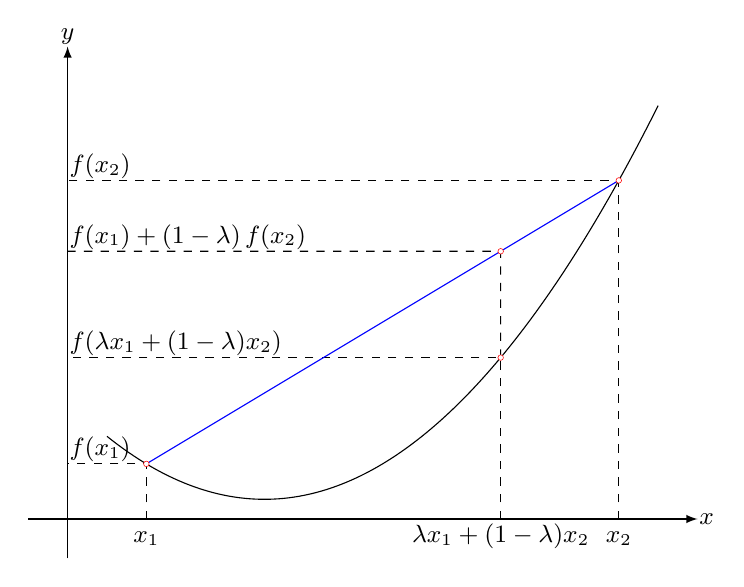
\begin{tikzpicture}[declare function={f(\x)=(\x-1)*(\x-1)/2 +
0.1;},x={(2.5cm,0)},y={(0,2.5cm)},samples=101,font=\small,inner sep=0.5pt]
\draw[-latex] (-0.2,0) -- (3.2,0)  node [right] {$x$};
\draw[-latex] (0,-0.2) -- (0,2.4) node [above] {$y$};
\coordinate (O) at (0,0);
\draw plot[domain=0.2:3,variable=\x] ({\x},{f(\x)});
\foreach [count=\Z] \X/\Y in {0.4/{x_1},2.2/{\lambda x_1 +(1-\lambda) x_2},2.8/{x_2}}
{\draw[dashed] (\X,0) coordinate (X\Z) node[below]{$\strut\Y$} -- (\X,{f(\X)}) coordinate (F\Z)
-- (0,{f(\X)}) node[above right]{$f(\Y)$};}
\draw[blue] (F1) -- (F3);
\draw[dashed] (F2) --
(intersection cs:first line={(X2)--(F2)}, second line={(F1)--(F3)})
coordinate (F4) -- (O|-F4) node[above right]{$f(x_1)+(1-\lambda)\,f(x_2)$};
\foreach \X in {1,...,4}
{\draw[very thin,red,fill=white] (F\X) circle(1pt);}
\end{tikzpicture}}
 \subfigure[Concave Function Example]{~\label{Fig:Concave_Function}
    \begin{tikzpicture}[scale=.7]
     \draw [->] (-1,-0.23) -- (11,-0.23) node [right] {$x$};
     \draw [->] (0,-1) -- (0,8) node [above] {$y$};
     \node at (0,-0.23) [below left] {$0$};
     \draw  plot[smooth, tension=.7] coordinates{(1.5,-0.5) (3,3) (5,1.5)  (7.5,4) (10,-1)};
     \node at (1.75,-0.5) {\scriptsize$a$};
     \node at (9.5,-0.5) {\scriptsize$b$};
     \draw[dashed] (3.2,3.05) -- (3.2,-0.23);
     \draw[dashed] (4.9,1.5) -- (4.9,-0.23);
     \draw[dashed] (7.3,4.05) -- (7.3,-0.23);
     \node at (3.2,-0.5) {\scriptsize$c_{1}$};
     \node at (4.9,-0.5) {\scriptsize$c_{2}$};
     \node at (7.3,-0.5) {\scriptsize$c_{3}$};
     \draw (2.5,3.05) -- (4,3.05);
     \draw (4,1.5) -- (6,1.5);
     \draw (6.5,4.05) -- (8.25,4.05);
     \node at (3.2,3.5) {\scriptsize$f'(c_{1})=0$};
     \node at (4.9,2.2) {\scriptsize$f'(c_{2})=0$};
     \node at (7.3,4.7) {\scriptsize$f'(c_{3})=0$};
     \node at (9.5,3) {\scriptsize$y=f(x)$};
\end{tikzpicture}
}
\caption{Convex and Concave functions examples.}
\end{figure}%
\subsubsection{Gradient Descent}

As we explained previously, we need to find the relation between X,Y from the input parameters \textbf{\textit{(w,b)}} which will make the cost function in Equation~\eqref{eq:cost_function} to the minimum. In other words we need to find the best value of \textbf{\textit{J(w,b)}} which will represent the relation and reduce the error between $y$ and $\widehat{y}$ So, we need to minimize \textbf{\textit{J(w,b)}}.%
%
\begin{figure}[t]
\begin{center}
\begin{figure}[H]
\begin{center}
    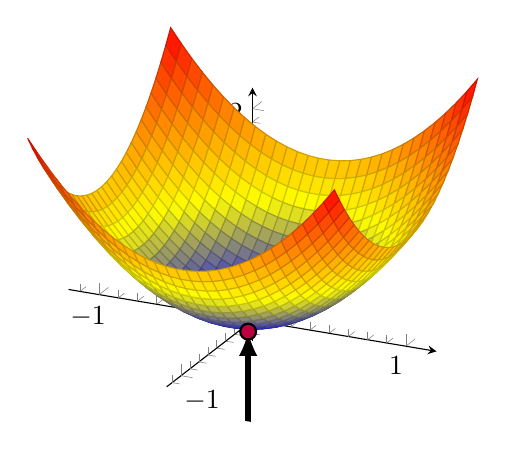
\begin{tikzpicture}
    %\draw[step=.5, gray!40, very thin] (0,0) grid (8,4);
\begin{axis}[axis lines=center,
       enlargelimits,
       tick align=inside,
       domain=-1:1,
       samples=30,
       minor tick num=7,]		
       \addplot3 [surf]{x^2+y^2};
       \draw[arrows=-latex,line width=2pt] (2.8cm,-5.2cm) -- (2.8cm,.23cm);
       \draw[thick,fill=purple] (2.8cm,.23cm) circle (0.1cm);
\end{axis}
\end{tikzpicture}
\caption{Gradient Decent }\label{fig:gradient_decent_surf}
\end{center}
\end{figure} 
\caption{Gradient Descent}\label{Fig:gradient_decent_surf}
\end{center}
\end{figure}%
%
To illustrate the relation between \textbf{\textit{J(w,b)}} we assume for simplicity the relation is a function of one variable \textbf{\textit{J(w)}}. As shown in Figure~\ref{Fig:gradient_decent_surf} we have a curve which represents the function \textbf{\textit{J(w)}} we need to find the minimum point in this curve which is the local minimum (red point in the previous figure) assuming it is a \textbf{\textit{convex function}}. we use Equation~\eqref{eq:gredient_descent_w} to find the local minimum.

To explain how this equation works, let's take a simple function $f(x) = x^2$, then select a random point $P_1$ from Figure~\ref{Fig:Derivative_Example}, then pick another point $P_2$. Let's take the derivative \textit{(which by definition is the slope of the function at the point which also the change between these two points)} The slope of this function is the height (3) divided by the width (1); this is the tangent of $J(w)=\frac{3}{1}$ at this point. If the derivative is positive, w will be update minus the derivative multiplied by learning rate alpha $\alpha$ as in Equation~\eqref{eq:gredient_descent_w}. We repeat the previous step until the value of w reaches the minimum. At this point, the derivative is negative, so w will start to increase again; at this step the algorithm will stop. Also, we can demonstrate the effect of different $\alpha$ values and their impact on the function; we can show this effect in Figure~\ref{Fig:Alpha_Change} but the main point is that it is not always a happy scenario. Sometimes the high $alpha$ is not a good idea; it depends on the problem and the dataset.

Now, let's generalize the above equation. Assume we have two parameters \textbf{\textit{(w,b)}} and we need to calculate the cost function for \textbf{\textit{J(w,b)}} we work on as two steps; first function in Equation~\eqref{eq:gradient_descent_j_w} wrt \textbf{\textit{(w)}}, and second function in Equation~\eqref{eq:gradient_descent_j_b} wrt \textbf{\textit{(b)}}%
%
\begin{figure}[!t]
\subfigure[Derivative Example of function $f(x) = x^2$]{~\label{Fig:Derivative_Example}
\begin{figure}[H]
\begin{center}
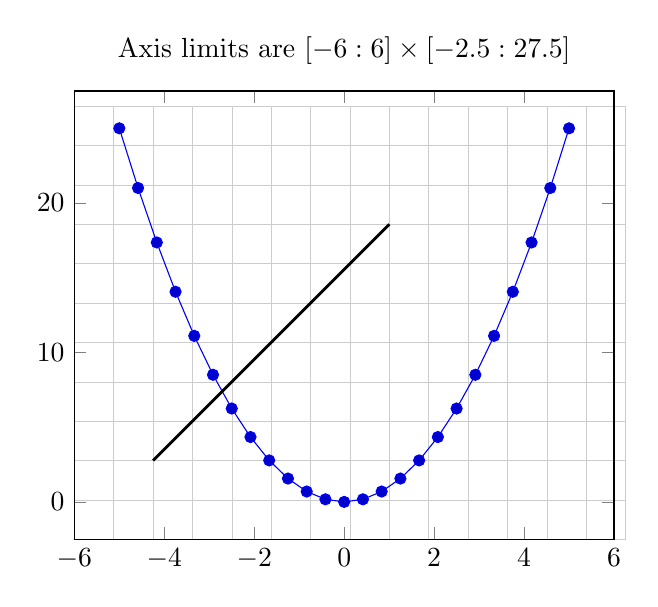
\begin{tikzpicture}
\draw[step=.5, gray!40, very thin] (0,0) grid (7,5.5);
\begin{axis}[
 % Show (automatically) computed limits:
 title={
  Axis limits are 
  $
 [\pgfmathprintnumber{\pgfkeysvalueof{/pgfplots/xmin}}
 :\pgfmathprintnumber{\pgfkeysvalueof{/pgfplots/xmax}}
 ]  \times 
 [\pgfmathprintnumber{\pgfkeysvalueof{/pgfplots/ymin}}
 :\pgfmathprintnumber{\pgfkeysvalueof{/pgfplots/ymax}}
 ]$ },
]
\addplot {x^2};
% \draw[arrows=-latex,line width=2pt] (2.8cm,-5.2cm) -- (2.8cm,.23cm);
% \draw[arrows=-latex,line width=1pt] (-.07 cm,4.8cm) -- (5.5cm,4cm);


\end{axis}
\draw[line width=1pt] (1,1) -- (4,4);
    \end{tikzpicture}
  
\caption{Derivative Example }\label{fig:derivative_example}
\end{center}
\end{figure} }
\subfigure[Derivative Example of function $f(x) = x^2$ where $\alpha_1$ > $\alpha_2$]{\label{Fig:Alpha_Change}
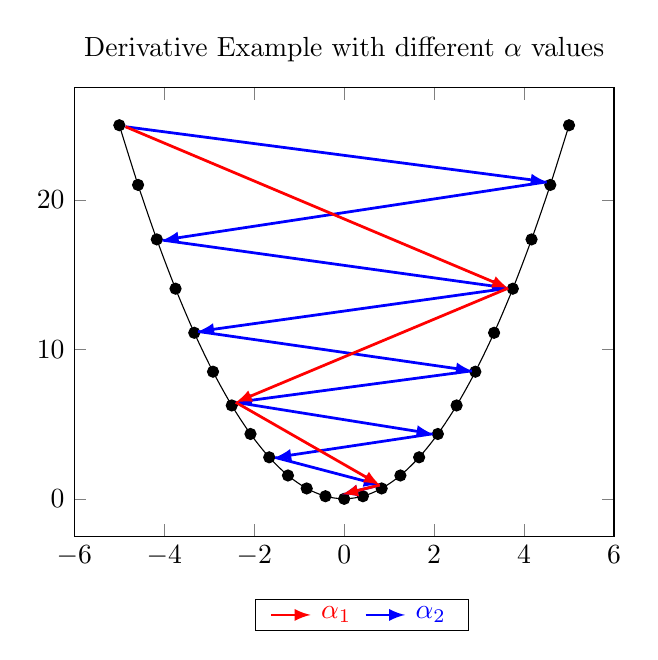
\begin{tikzpicture}
%\draw[step=.5, gray!40, very thin] (0,0) grid (7,5.5);
\begin{axis}[
% Show (automatically) computed limits:
title={
	Derivative Example with different $\alpha$ values},]
\addplot[mark=*,black,smooth] {x^2};
%\addlegendentry{$f(x)=x^2$};
%\addlegendimage{only marks,mark=*};
%\addlegendimage{only marks,mark=diamond*};
\end{axis}

\draw[arrows=-latex,line width=1pt,blue] (.65,5.2) -- (6,4.5);
\draw[arrows=-latex,line width=1pt,blue] (6,4.5) -- (1.12,3.76);
\draw[arrows=-latex,line width=1pt,blue] (1.12,3.76) -- (5.51,3.15);
\draw[arrows=-latex,line width=1pt,blue] (5.51,3.15)--(1.57,2.6);
\draw[arrows=-latex,line width=1pt,blue] (1.57,2.6)--(5.05,2.1);
\draw[arrows=-latex,line width=1pt,blue] (5.05,2.1)--(2.05,1.7);
\draw[arrows=-latex,line width=1pt,blue] (2.05,1.7) -- (4.55,1.3) ;
\draw[arrows=-latex,line width=1pt,blue]  (4.55,1.3) --(2.55,1);
\draw[arrows=-latex,line width=1pt,blue]  (2.55,1)--(3.88,.65);
\draw[arrows=-latex,line width=1pt,blue]  (3.88,.65)--(3.4,.53);

\draw[arrows=-latex,line width=1pt,red] (.65,5.2) -- (5.51,3.15);
\draw[arrows=-latex,line width=1pt,red] (5.51,3.15)--(2.05,1.7);
\draw[arrows=-latex,line width=1pt,red]  (2.05,1.7) --(3.88,.65);
\draw[arrows=-latex,line width=1pt,red]  (3.88,.65)--(3.4,.53);
\draw[arrows=-latex,line width=1pt,red]  (2.5,-1)-- (3,-1) node [right] {$\alpha_1$};
\draw[arrows=-latex,line width=1pt,blue]  (3.7,-1)-- (4.2,-1) node [right] {$\alpha_2$};
\draw  (2.3, -1.2) rectangle (5, -0.8);


\end{tikzpicture}
}
\end{figure}%
%
\begin{equation}\label{eq:gredient_descent_w}
 \begin{split}
  w & := w - \alpha dw \quad \text{\textit{alpha is learning rate}}\\
   & := w - \alpha \frac{dJ(w)}{dw} \quad \text{\textit{d represent the derivative wrt w}}
 \end{split}
\end{equation}
%
\begin{subequations}
   \begin{align}
w& := w - \alpha \frac{dJ(w,b)}{dw} \label{eq:gradient_descent_j_w}\\
b& := b - \alpha \frac{dJ(w,b)}{db} \label{eq:gradient_descent_j_b}
   \end{align}
 \end{subequations}
%
\subsubsection{Logistic Regression derivatives}\label{Sec:Logistic_Bp_Derivatives}

As described, we need to calculate the gradient descent to get the best $\widehat{y}$ which minimizes the total cost in equation~\eqref{eq:logistic_regression_derivatives_single_example}. So, doing back propagation to get the value of $dz$, we need to calculate $da$ in Equation~\eqref{eq:logistic_regression_derivatives_da}, then calculate $dz$ based on the output of $da$ from Equation~\eqref{eq:logistic_regression_derivatives_dz}. After that, we start to take the derivative for $z$ function parameters \textbf{\textit{$w_1,w_2,b$}}. Once we have the values of \textbf{\textit{$dw_1,dw_2,db$}} we can use them to calculate the estimated values of \textbf{\textit{$w_1,w_2,b$}} in Equations~\eqref{eq:logistic_regression_derivatives_dw1},~\eqref{eq:logistic_regression_derivatives_dw2},~\eqref{eq:logistic_regression_derivatives_db}.%
%
\begin{equation}\label{eq:logistic_regression_derivatives_single_example}
  \boxed{\widehat{y} = \sigma(z) = a} \longrightarrow \boxed{ z = w^tx + b = w_1x_1+ w_2+x_2+ b} \longrightarrow \boxed{\ell(a,y)}
 \end{equation}
 \begin{equation}\label{eq:logistic_regression_derivatives_da}
   \boxed{da = \frac{d\ell}{da} = \frac{d\ell(a,y)}{da} = - \frac{y}{a} + \frac{1-y}{1-a}}
 \end{equation}
  \begin{equation}\label{eq:logistic_regression_derivatives_dz}
  \boxed{dz = \frac{d\ell}{dz} = \frac{d\ell(a,y)}{dz} = \frac{d\ell}{da} . \frac{da}{dz}} = \boxed{(- \frac{y}{a} + \frac{1-y}{1-a}) . a(a-1) } = \boxed{ a - y  }
 \end{equation}
 \begin{equation}\label{eq:logistic_regression_derivatives_dw1}
   \boxed{dw_1 = \frac{\partial\ell}{dw_1} = x_1 dz} \longrightarrow \boxed{ w_1 := w_1 - \alpha dw_1}
 \end{equation}
  \begin{equation}\label{eq:logistic_regression_derivatives_dw2}
  \boxed{dw_2 = \frac{\partial\ell}{dw_2} = x_2 dz} \longrightarrow \boxed{ w_2 := w_2 - \alpha dw_2}
 \end{equation}
 \begin{equation}\label{eq:logistic_regression_derivatives_db}
  \boxed{db = \frac{\partial\ell}{db} = dz} \longrightarrow \boxed{ b := b - \alpha db}
\end{equation}%
%
\subsubsection{Implementing Logistic Regression on m example}
To implement a simple 1 iteration, in the example below the sample code simulates the program structure. First, assume $J = 0, dw_1 = 0, dw_2 = 0,db = 0$. Then calculate the feedforward step. Then backpropagation calculate. Finally, update the parameters. We can transfer the above equation into the below python sample code.%
 \begin{lstlisting}[language=Python]
  import numpy as np
  J = 0, dw_1 = 0, dw_2 = 0,db = 0, alpha = .02
  # FEED FORWARD PROPAGATION
  A = 1 / (1 + np.exp(-(np.dot(w.T,X) + b))#  Z = np.dot(w.T,X) + b
  cost = (- 1 / m) * np.sum(Y * np.log(A) + (1 - Y) * (np.log(1 - A)))
  # BACKWARD PROPAGATION (TO FIND GRADIENT)
  dw = (1 / m) * np.dot(X, (A - Y).T) #  dz = A - Y
  db = (1 / m) * np.sum(A - Y)
  # UPDATE THE PARAMETERS
  w = w - alpha * dw
  b = b - alpha * db
 \end{lstlisting}%
%
\subsection{The Neuron}

Most computer research is trying to simulate the human brain as it is the most advanced creation. If we are trying to check how the model understands the new information, we can give a baby two bananas then ask him about them. The baby can remember it with all it new shapes. Similarly, if you inform any human about some information and trying to get a new inference, it will automatically detect this information. So, the new research tries to simulate the human brain model into an Artificial Intelligence model to achieve this performance. In this subsection, we try to give an overview of the relation between the new research era and the human brain.
 
The neuron is the foundation unit of the brain. The size of the brain is about the size of a grain of rice. The brain contains over 10000 neurons with average 6000 connections with other neurons~\cite{Restak_2001}.  These massive networks allow our brain to build its knowledge about the world around us. The neuron works by receiving the information from other neurons and processes it uniquely then passes the output to other neurons; this process is shown in Figure~\ref{Fig:Neuron_Structure}.%

\begin{figure}[!t] 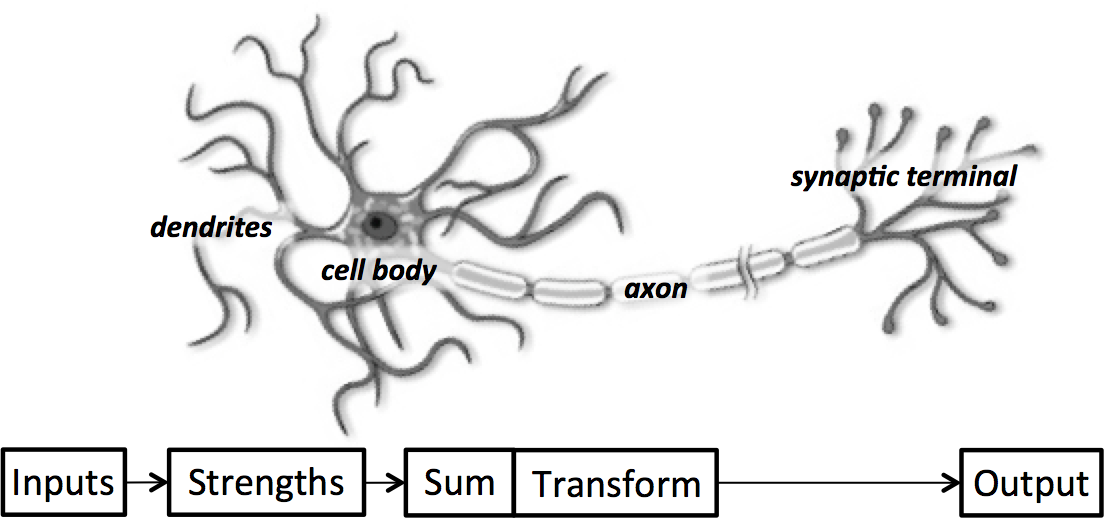
\includegraphics[width=\linewidth]{./Figures/Ch_2_Background/neuron_structure.png}
\caption{Description of neuron's structure this figure from~\cite{DLFundamentals}}
~\label{Fig:Neuron_Structure}
\end{figure}%
 
How do we learn a new concept? \textit{The neuron receives its input from dendrites. The incoming neuron connection is dynamically strengthened or weakened based on how often it is used, and the strength of each connection determines the contribution of the input to the neuron's output. Based on the connection strength, it has weight then the input is summed in the cell body. This sum is transformed into a new signal which is propagated along the cell's axon and sent to other neurons~\cite{DLFundamentals}}.

The above biological model can be translated into an Artificial Neural Network as described in figure~\ref{Fig:NNExample}. We have an input $x_1,x_2,x_3,...,x_n$; every input has its own strength (weight) $w_1,w_2,w_3,...,w_n$. We sum the multiplication of X and W to get the logit of the neuron, $z =  \sum_{i=0}^{n} x_i w_i $. The logit is passed through a function $f$ to produce the output $ y = f(z)$. The output will be the input to other neurons. Note: in many cases, the logit can also include a bias constant. So, in this case the function will be $$ y = f(\sum_{i=0}^{n} x_i w_i + b)$$.
 
\subsection{The Neural Network Representation}
As explained previously, we have been trying to simulate the human brain model into our research work in Deep Neural Network. So, we have multi-layers to allow the model to get in-depth knowledge and more computational performance to simulate the human brain. 

Now, we represent the functions per layer as per the equations below where lt refers to layer number, i refers to the node number in the layer~\eqref{eq:nn_multi_layer}%
%
\begin{equation}\label{eq:nn_multi_layer}
\boxed{z^l = W^l x + b^l} \longrightarrow \boxed{a_i^l = \sigma(z^l)} \longrightarrow \boxed{\ell(a^l,y)}
\end{equation}%
%
What is the Neural Networks component?
Figure~\ref{Fig:NNExample} represents an Example of Neural Networks representations. It consists of

\begin{itemize}
\item \textbf{Input Layer:} Input layer is the input data raw for the network, denoted as $a^0$.
\item \textbf{Hidden Layers:} The layers between the input layers and the output layer can be any number of layers.These have a set of weighted input and produce an output through an activation function. Every layer in the hidden layer transmits the output to the other hidden layer as an input feature.
\item \textbf{Output Layer:} This is one output layer with the final results from the hidden layers.
\end{itemize}

\subsection{Neural Network Computation}

In this subsection, we show as example on how we can compute the Neural Networks for every layer. In figure~\ref{Fig:NNExample} we have an example of Input layer of N input, one hidden layer, and one output layer. We continue explain on this example in Equation~\eqref{eq_nn_one_layer}.%
\begin{figure}[!t]
\begin{tikzpicture}
\node[draw,circle,minimum size=25pt,inner sep=0pt] (x) at (0,0) {$\Sigma$ $\sigma$};

\node[inputNode] (x0) at (-2, 1.5) {$\tiny +1$};
\node[inputNode] (x1) at (-2, 0.75) {$\tiny x_1$};
\node[inputNode] (x2) at (-2, 0) {$\tiny x_2$};
\node[inputNode] (x3) at (-2, -0.75) {$\tiny x_3$};
\node[inputNode] (xn) at (-2, -1.75) {$\tiny x_n$};

\draw[stateTransition] (x0) to[out=0,in=120] node [midway, sloped, above] {$w_0$} (x);
\draw[stateTransition] (x1) to[out=0,in=150] node [midway, sloped, above] {$w_1$} (x);
\draw[stateTransition] (x2) to[out=0,in=180] node [midway, sloped, above] {$w_2$} (x);
\draw[stateTransition] (x3) to[out=0,in=210] node [midway, sloped, above] {$w_3$} (x);
\draw[stateTransition] (xn) to[out=0,in=240] node [midway, sloped, above] {$w_n$} (x);
\draw[stateTransition] (x) -- (4,0) node [midway,above] {$\sigma\left(w_0 + \sum\limits_{i=1}^{n}{w_ix_i}\right)$};
\draw[dashed] (0,-0.43) -- (0,0.43);
\node (dots) at (-2, -1.15) {$\vdots$};
\node[inputNode, thick] (i1) at (6, 0.75) {};
\node[inputNode, thick] (i2) at (6, 0) {};
\node[inputNode, thick] (i3) at (6, -0.75) {};

\node[inputNode, thick] (h1) at (8, 1.5) {};
\node[inputNode, thick] (h2) at (8, 0.75) {};
\node[inputNode, thick] (h3) at (8, 0) {};
\node[inputNode, thick] (h4) at (8, -0.75) {};
\node[inputNode, thick] (h5) at (8, -1.5) {};

\node[inputNode, thick] (o1) at (10, 0.75) {};
\node[inputNode, thick] (o2) at (10, -0.75) {};

\draw[stateTransition] (5, 0.75) -- node[above] {$I_1$} (i1);
\draw[stateTransition] (5, 0) -- node[above] {$I_2$} (i2);
\draw[stateTransition] (5, -0.75) -- node[above] {$I_3$} (i3);

\draw[stateTransition] (i1) -- (h1);
\draw[stateTransition] (i1) -- (h2);
\draw[stateTransition] (i1) -- (h3);
\draw[stateTransition] (i1) -- (h4);
\draw[stateTransition] (i1) -- (h5);
\draw[stateTransition] (i2) -- (h1);
\draw[stateTransition] (i2) -- (h2);
\draw[stateTransition] (i2) -- (h3);
\draw[stateTransition] (i2) -- (h4);
\draw[stateTransition] (i2) -- (h5);
\draw[stateTransition] (i3) -- (h1);
\draw[stateTransition] (i3) -- (h2);
\draw[stateTransition] (i3) -- (h3);
\draw[stateTransition] (i3) -- (h4);
\draw[stateTransition] (i3) -- (h5);

\draw[stateTransition] (h1) -- (o1);
\draw[stateTransition] (h1) -- (o2);
\draw[stateTransition] (h2) -- (o1);
\draw[stateTransition] (h2) -- (o2);
\draw[stateTransition] (h3) -- (o1);
\draw[stateTransition] (h3) -- (o2);
\draw[stateTransition] (h4) -- (o1);
\draw[stateTransition] (h4) -- (o2);
\draw[stateTransition] (h5) -- (o1);
\draw[stateTransition] (h5) -- (o2);

\node[above=of i1, align=center] (l1) {Input \\ layer};
\node[right=2.3em of l1, align=center] (l2) {Hidden \\ layer};
\node[right=2.3em of l2, align=center] (l3) {Output \\ layer};

\draw[stateTransition] (o1) -- node[above] {$O_1$} (11, 0.75);
\draw[stateTransition] (o2) -- node[above] {$O_2$} (11, -0.75);

\path[dashed, double, ultra thick, gray] (x.north) edge[bend left=0] (h5.north);
\path[dashed, double, ultra thick, gray] (x.south) edge[bend right=0] (h5.south);
\end{tikzpicture}

\caption{Neural Networks Example Input layer with N input samples, One hidden Layer, and an Output Layer}~\label{Fig:NNExample}
\end{figure}%
\begin{subequations}\label{eq_nn_one_layer}
\begin{align}
Z_1^{[1]} & = w_1^{[1]T} x + b_1^{[1]} , a_1^{[1]} = \sigma(Z_1^{[1]}) \\
Z_2^{[1]} & = w_2^{[1]T} x + b_2^{[1]} , a_2^{[1]} = \sigma(Z_2^{[1]})\\
Z_3^{[1]} & = w_3^{[1]T} x + b_3^{[1]} , a_3^{[1]} = \sigma(Z_3^{[1]})\\
Z_4^{[1]} & = w_4^{[1]T} x + b_4^{[1]} , a_4^{[1]} = \sigma(Z_4^{[1]})
\end{align}
\end{subequations}%

If we need to compute the above equations, it is simply be represented as vectorized. The matrix below shows how we can implement it.%
\[
z^{[1]} = 
\left[
 \begin{array}{ccc}
   w^{[1]T}_{1} \\
   w^{[1]T}_{2} \\
   w^{[1]T}_{3} \\
   w^{[1]T}_{4} \\ 
 \end{array}
\right]\cdot
\left[
 \begin{array}{c}
  x_{1} \\
  x_{2} \\
  x_{3} %\vdots \\
 \end{array}
\right] +
\left[
 \begin{array}{c}
  b_{1}^{[1]}\\
  b_{2}^{[1]}\\
  b_{3}^{[1]}\\
  b_{4}^{[1]}
 \end{array}
\right] =
\left[
 \begin{array}{cccc}
   w^{[1]T}_{1} x + b _1^{[1]}\\
   w^{[1]T}_{2} x + b _2^{[1] }\\
   w^{[1]T}_{3} x + b _3^{[1] }\\
   w^{[1]T}_{4} x + b _4^{[1] }\\ 
 \end{array}
\right] =
\left[
 \begin{array}{c}
  z_1^{[1]} \\
  z_2^{[1]} \\
  z_3^{[1]} \\
  z_3^{[1]}
 \end{array}
\right]
\]%
\subsubsection{Linear Neurons and Their Limitations}

We explained the equations for the feedforward Neural Network. We have only one point we need to discuss, which is the Activation function. Let's assume we continue using linear function in Figure~\ref{Fig:Linear}, which represents linear equation  $y= w x + b$. So, if we have mutli-layer networks, for example Equation~\eqref{eq:linear_fun_limitations}, it will end as linear function because composition of two linear function will be linear function. So, we do not compute deep computation and we get limited information from the networks. So, to be able to detect the deep information we use different functions for the hidden layers, for example: $\tanh$ Figure~\ref{Fig:Tanh} and its Equation~\eqref{eq:nn_tanh}. Another option is Sigmoid Figure~\ref{Fig:Sigmoid} and  Equation~\eqref{eq:logistic_function}. Finally, Relu Figure~\ref{Fig:Relu} Equation~\eqref{eq:nn_relu}. Most binary classification problems use Sigmoid function for output layer. We can use the same functions for the output but we can also use the linear for activation function in some cases.%
\begin{figure}[!t]
 \centering
 \subfigure[RELU activation function.]{\label{Fig:Relu}
  \begin{tikzpicture}
   \begin{axis}[
    xmin=-2.5, xmax=2.5,
    ymin=-1.5, ymax=1.5,
    axis lines=center,
    axis on top=true,
    domain=-2.5:2.5,
    ylabel=$y$,
    xlabel=$x$,
    ]

    \addplot [mark=none,draw=blue,smooth] {ifthenelse(
                    x<0,        % if
                    0,          % then
                    x           % else
                )
    %abs(tanh(\x))
    };
    \node [right, blue] at (axis cs: 1,0.7) {$y = relu(x)$};

    %% Add the asymptotes
    %\draw [blue, dotted, thick] (axis cs:-2.5,-1)-- (axis cs:0,-1);
    %\draw [blue, dotted, thick] (axis cs:+2.5,+1)-- (axis cs:0,+1);
    
\end{axis}
  \end{tikzpicture}}
%
 \subfigure[Tanh activation function.]{\label{Fig:Tanh}
  \begin{tikzpicture}
   \begin{axis}[
    xmin=-2.5, xmax=2.5,
    ymin=-1.5, ymax=1.5,
    axis lines=center,
    axis on top=true,
    domain=-2.5:2.5,
    ylabel=$y$,
    xlabel=$x$,
    ]

    \addplot [mark=none,draw=blue,smooth] {tanh(\x)};
    \node [right, blue] at (axis cs: 1,0.7) {$y = \tanh x$};

    %% Add the asymptotes
    %\draw [blue, dotted, thick] (axis cs:-2.5,-1)-- (axis cs:0,-1);
    %\draw [blue, dotted, thick] (axis cs:+2.5,+1)-- (axis cs:0,+1);
    
\end{axis}
  \end{tikzpicture}}
% 
\subfigure[Linear activation function.]{\label{Fig:Linear}
  \begin{tikzpicture}
   \begin{axis}[
    xmin=-2.5, xmax=2.5,
    ymin=-1.5, ymax=1.5,
    axis lines=center,
    axis on top=true,
    domain=-2.5:2.5,
    ylabel=$y$,
    xlabel=$x$,
    ]

    \addplot [mark=none,draw=blue,smooth] {\x +.5};
    \node [right, blue] at (axis cs: 1,0.7) {$y = x +.5$};

    %% Add the asymptotes
    %\draw [blue, dotted, thick] (axis cs:-2.5,-1)-- (axis cs:0,-1);
    %\draw [blue, dotted, thick] (axis cs:+2.5,+1)-- (axis cs:0,+1);
    
\end{axis}
  \end{tikzpicture}}
%
\subfigure[Logistic sigmoid activation function.]{\label{Fig:Sigmoid}
  \begin{tikzpicture}
   \begin{axis}[
    xmin=-2.5, xmax=2.5,
    ymin=-1.5, ymax=1.5,
    axis lines=center,
    axis on top=true,
    domain=-2.5:2.5,
    ylabel=$y$,
    xlabel=$x$,
    ]

    \addplot [mark=none,draw=blue,smooth] {1/(1+exp(-\x))};
    \node [right, blue] at (axis cs: .8,1.1) {$y = \frac{1}{1+\exp(-x)}$};

    %% Add the asymptotes
    %\draw [blue, dotted, thick] (axis cs:-2.5,-1)-- (axis cs:0,-1);
    \draw [blue, dotted, thick] (axis cs:+2.5,+.5)-- (axis cs:0,+.5);
    
\end{axis}
  \end{tikzpicture}}
 \caption{Commonly used activation functions including the logistic sigmoid $\sigma(z)$, the hyperbolic tangent $\tanh(z)$, the rectified hyperbolic tangent RelU $Relu(x)$, and linear function}
\end{figure}%
\begin{subequations}\label{eq:linear_fun_limitations}
  \begin{align}
   Z^{[1]} & = w_1^{[1]T} x + b_1^{[1]} , a_1^{[1]} = \sigma(Z_1^{[1]}) \\
   Z^{[2]} & = w^{[2]T} a^1 + b^{[2]} = w^{[2]T} (w^{[1]T}x + b^{[1]}) + b^{[2]}\\
   & = (w^{[1]T}W^{[2]T})x + (w^{[2]}b^{[1]}+ b^{[2]})\\
   & = W' x + b'
\end{align}
\end{subequations}%
\begin{equation}\label{eq:nn_tanh}
 a = \tanh(z) =\frac{e^z-e^{-z}}{e^z+e^{-z}}
\end{equation}%
\begin{equation}\label{eq:nn_relu}
 a = \max(0,z)
\end{equation}%
%
\subsubsection{Softmax Output Layers}
Sometimes our problem has multi-output results, not only 1 or 0. For example, we have a problem recognizing the characters from 0 to 9 in MNIST dataset, But we are unable to recognize digits with 100\% confidence. So, we use the probability distribution to give us a better idea of how confident we are in our predictions. The result will be an output vector of the form of the $\sum_{i = 0}^9P_i=1$.

This is achieved by using a special output layer named softmax layer. This layer differs from the other as the output of a neuron in a softmax layer depends on the output of all the other neurons in its layer. This because its sum of all output equal 1. If we assume $z_i$ be the logit of $i^{th}$ softmax neuron, we can normalize by setting its output to represented from Equation~\eqref{eq:nn_softmax_fun}.%
\begin{equation}\label{eq:nn_softmax_fun}
 y_i=\frac{e^{z_i}}{\sum_je^{z_j}}
\end{equation}
%
The strong prediction will have a value entry in the vector close to 1, while the other entries will be close to 0. The weak prediction will have multiple possible labels, having almost equal values~\cite{DLFundamentals}.

\subsubsection{Forward-Propagation in a Neural Networks}
As an example, in Figure~\ref{Fig:NN_With_BP} we need to calculate the Forward propagation; we follow the equation~\eqref{eq:feedfarward_dL}. Note: we assume $X = a^{[0]}$ as initial function notation. Also, $\widehat{Y}= g(Z^{[4]}=A^{[4]}$ as the final output layer.%
\begin{equation}\label{eq:feedfarward_dL}
Z^{[l]} = w^{[l]} a^{l-1} + b^{[l]} , A^{[1]} = g^{l}(Z^{[l]})
\end{equation} % @@@ figure to show the input forward and back propagation steps

\begin{figure}[t]
\begin{tikzpicture}[%
  shorten >=1pt,->,draw=black!50, node distance=2.5cm,
  %every pin edge={<-,shorten <=1pt},
  neuron/.style={circle,fill=black!25,minimum size=17pt,inner sep=0pt},
  input neuron/.style={neuron, fill=green!50},
  output neuron/.style={neuron, fill=red!50},
  hidden neuron/.style={neuron, fill=blue!50},
  annot/.style = {text width=4em, text centered}
  ]
  \def\layersep{2.5cm}
  % Draw the input layer nodes
  \foreach \name / \y in {1,...,4}
  % This is the same as writing \foreach \name / \y in {1/1,2/2,3/3,4/4}
  \node[input neuron, pin={[pin edge={<-,shorten <=1pt}]left:Input \#\y}] (I-\name) at (0,-\y) {};

  % Draw the hidden layer nodes
  \foreach \name / \y in {1,...,5}
  \node[hidden neuron] (H-\name) at (\layersep,-\y cm+0.5cm) {};

  % Draw the output layer node
  \node[output neuron,pin={[pin edge={->}]right:Output}, right=of H-3] (O) {};

  % Connect every node in the input layer with every node in the
  % hidden layer.
  \foreach \source in {1,...,4}
  \foreach \dest in {1,...,5}
  \path (I-\source) edge (H-\dest);

  % Connect every node in the hidden layer with the output layer
  \foreach \source in {1,...,5}
  \path (H-\source) edge (O);

  % Annotate the layers
  \node[annot,above=15mm of H-1] (hl) {Hidden layer};
  \node[annot,left=of hl] {Input layer};
  \node[annot,right=of hl] {Output layer};
  %%% 
  \coordinate (H-I-1) at ($(H-1)!0.5!(I-1)$);
  \draw (O) |- ($(H-I-1) +(0,1)$) node[above,pos=0.75]{Back propagation} -- (H-I-1);
  \draw ;
\end{tikzpicture}
\caption{Neural Network Example with Backpropagation Step.}~\label{Fig:NN_With_BP}
\end{figure}%
\subsubsection{Back-Propagation in a Neural Networks}

To compute the gradient descent in Neural Networks, we use an algorithm named \textit{backpropagation}. The backpropagation algorithm was initially invented in the 1970s, but was relatively unknown until one of the most important papers in this field was published in 1986, describing several neural networks where backpropagation has a performance significantly better than the earlier approaches and making it possible to use neural networks to solve problems which were previously insoluble. Backpropagation is now the backbone for the learning in neural networks.
%@@@MUSTcite https://www.nature.com/articles/323533a0
We explained previously, how neural networks could learn their weights using gradient descent algorithm. In this part, we explain how to compute the gradient of the cost function.
%@@@cite Michael A. Nielsen, "Neural Networks and Deep Learning", Determination Press, 2015

Backpropagation not only an algorithm which gives us the expression for partial derivative of the cost function $C$ with respect to weights $w$ and bias $b$, but also suggests possibilities about the change of the cost function while changing its variables $w \& b$ and its effect on the overall network~\ref{Fig:NN_With_BP}.

As explained in the Logistic Regression section (\ref{Sec:Logistic_Bp_Derivatives}), we can calculate the derivatives for logistic regression with one layer using this equations~\eqref{eq:logistic_regression_derivatives_single_example},~\eqref{eq:logistic_regression_derivatives_da},~\eqref{eq:logistic_regression_derivatives_dz},\\
~\eqref{eq:logistic_regression_derivatives_dw1},~\eqref{eq:logistic_regression_derivatives_dw2},~\eqref{eq:logistic_regression_derivatives_db}.\\

we generalize the derivatives equations to be for $l$ layers from the equations below~\eqref{eq:nn_bp_l_layers}.%
%
\begin{subequations}\label{eq:nn_bp_l_layers}
  \begin{align}
   dz^{[l]} & = da^{[l]} \times g^{[l]'}(z^{l}) \\
   dw^{[l]} & = dz^{[l]} \cdot a^{[l-1]} \\
   db^{[l]} & = dz^{[l]} \\
   da^{[l-1]} & = W^{[l]T} \cdot dz^{[l]} %\\
%   dz^{[l]} & = (W^{[l+1]T} \cdot dz^{[l+1]}) * g^{[l]'}(z^{l}) \quad \text{from 2.24d in 2.24a}
 \end{align}
\end{subequations}%
We can vectorize the above equation for Neural Network implementation as per the equations below~\eqref{eq:nn_bp_l_layers_vectorize}.
 \begin{subequations}\label{eq:nn_bp_l_layers_vectorize}
  \begin{align}
   dz^{[l]} & = dA^{[l]} \times g^{[l]'}(z^{l}) \\
   dw^{[l]} & = \frac{1}{m} dz^{[l]} \cdot A^{[l-1]T} \\
   db^{[l]} & = \frac{1}{m} \text{ np.sum(}dz^{[l]}\text{,axis=1,keepdims = true)} \\
   dA^{[l-1]} & = W^{[l]T} \cdot dz^{[l]} %\\
%   dz^{[l]} & = (W^{[l+1]T} \cdot dz^{[l+1]}) * g^{[l]'}(z^{l}) \quad \text{from 2.24d in 2.24a}
 \end{align}
\end{subequations}%
%
If we check the input variable in the backpropagation we find it is $da^{l}$ and this is the derivative of~\eqref{eq:loss_function} which we can find, as explained previously from~\eqref{eq:logistic_regression_derivatives_da}; this is the formula for the final layer in the feedforward step. If we need to calculate the vectorized version of this equation, we can use equation~\eqref{eq:logistic_regression_derivatives_da_vectorize}
\begin{equation}\label{eq:logistic_regression_derivatives_da_vectorize}
da = \frac{d\ell}{da} = \frac{d\ell(a,y)}{da} = (- \frac{y^{[1]}}{a^{[1]}} + \frac{1-y^{[1]}}{1-a^{[1]}} \ldots - \frac{y^{[m]}}{a^{[m]}} + \frac{1-y^{[m]}}{1-a^{[m]}} )
\end{equation}%
%
\subsubsection{How we Initialize the Weights}
As explained previously in Logistic Regression, we initialized the weights to Zero. However, in Deep Neural Networks this will not work. Note: It is acceptable to initialize the Bias to Zero but for the weights it will not work. Let's see what happens if we initialize the weights and Bias to Zero. %@@@https://www.coursera.org/learn/neural-networks-deep-learning/lecture/XtFPI/random-initialization figure
  
Assume  we have two input vectors $x_1,X_2$, if we initialize $W^{[1]}$ to Zero from equation~\eqref{eq:nn_weights_init_zero} and $b^{[1]}$ to Zeros. So, $a_1^{[1]}=a_2^{[1]}$ because both of the hidden units compute the same functions. Also, $W^{[2]}=[0 0]$ Then, when we compute the backpropagation, we find that $dz_1^{[1]}=dz_2^{[2]}$. After every iteration, we find that the two hidden units calculate the same function and we do not obtain more information from this Deep Neural Network. We need to highlight that the main idea from Neural Networks, as explained before, is that every hidden unit should work to get a new piece of information. The more hidden units, the more hidden information we obtain, but if we initialize it to Zero, it will be the same function which is calculated, and we do not derive any new information.%
%
\begin{subequations}\label{eq:nn_weights_init_zero}
\begin{align}
 W^{[1]} = \begin{bmatrix} 0 & 0\\ 0 & 0 \end{bmatrix} \quad b^{[1]} = \begin{bmatrix} 0 \\ 0 \end{bmatrix} \\
 W^{[2]} = \begin{bmatrix} 0 & 0 \end{bmatrix} \\
 a_1^{[1]} = a_2^{[1]} \quad   dz_1^{[1]} = dz_2^{[1]}\\
 dw = \begin{bmatrix} u & u \\ v & v \end{bmatrix} \quad W^{[1]} = W^{[1]} - \alpha dw
\end{align}
\end{subequations}%
%
To initialize weights and to get the maximum value of the neural network computation, we should initialize the weight by small random numbers to avoid the big weights which will tend to cause a small slope from the Z where $Z^{[1]}= W^{[1]} X + b^{[1]}$ For example, if we use $\tanh$ we produce big tail values $a^{[1]}= g^{[1]}(Z^{[1]})$. So, big weights are more likely to produce slow learning rate. 

\subsubsection{Regularization}

One of the most common problems anyone working with data science in general or deep learning faces is the overfitting problem. In statistics, overfitting is the production of an analysis that corresponds too closely or exactly to a particular set of data, and may, therefore, not fit additional data or predict future observations reliably~\cite{Wiki_Overfitting}. An overfitted model is a statistical model that contains more parameters that can be justified by the data. The essence of overfitting is to have unknowingly extracted residual variation (i.e. the noise) as if that variation represented underlying model structure. As a practical example,a  model performs adequately on training data but cannot predict test data. This means that the models are often free of bias in the parameter estimators, but have estimated (and actual) sampling variances that are needlessly large in the training and unable to be generalized to predict testing data. Figure~\ref{Fig:Fitting} shows different ways of fitting, We need to avoid both underfitting and overfitting. We attempted to enhance the results in our training sets, where the model is more complex, so that the training error reduces but the testing error does not. While building the neural networks, the more complex models lead to more overfitting problems.%
%
\begin{figure}[!ht]
\centering
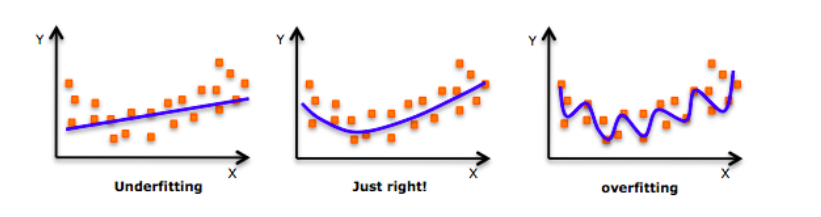
\includegraphics[scale=0.6]{./Figures/Ch_2_Background/Fig_Fitting.png}
\caption{Comparison Between different fitting types}~\label{Fig:Fitting}
\end{figure}%
%
We can enhance the results on testing data by getting more sample data. Therefore, the model can learn the pattern from the data in a better way, but sometimes it is difficult to acquire more data, or it is more expensive than the enhancement required. Hence, we work to apply regularization techniques to prevent overfitting.

Regularization is a technique which applies slight changes or modifications to the algorithm to be more generalized. Sometimes we try to hide information or add noise on the training data to avoid overfitting in the training phase. This considerably improves the model performance in the testing data or unseen.

\paragraph{Different Regularization Techniques in Deep Learning}

In this part, we explain how to apply different regularization techniques in deep learning.

\begin{itemize}
\item \textbf{L2 \& L1 Regularization} are the most common types of regularization. They update the general cost function by adding another term~\eqref{eq:regularization} known as the regularization term~\cite{Web_Analyticsvidhya_Regularization}.
\begin{equation}\label{eq:regularization}
J(w,b) = \ell(y,\widehat{y}) + Regularization
\end{equation}
%
Addition of this regularization term decreases the values of weight matrices. This happens because it assumes that a neural network with smaller weight matrices leads to simpler models. Therefore, it will also reduce overfitting to a significant extent. Assuming we reduce the value of $\lambda$ to be close to zero, this will produce a simpler network and many nodes will be equal zeros. This will reduce the high variance  and hence be less prone to overfitting.%
\begin{enumerate}
\item L2 regularization is the most common type of regularization. In L2 regularization we add $\lambda$ as regularization parameter. This  hyperparameter value is optimized for better results~\eqref{eq:regularization_l2}. It also known as weight decay as it forces the weights to decay towards zero (but not exactly zero)~\cite{Web_Analyticsvidhya_Regularization}.%
\begin{equation}\label{eq:regularization_l2}
J(w,b) = \frac{1}{m} \sum_{i=1}^{m} \ell(y,\widehat{y})+\frac{\lambda}{2m} \times \lVert w \rVert^2
\end{equation}%
\item In L1 Regularization, We penalize the absolute value of the weights~\eqref{eq:regularization_l1}. If we use L1 regularization $W$ can end up being sparse which means $w$ vector will have a lot of zeros. This can help to compress the model because the set of parameters are zero and we need less memory to store the model. Otherwise, we usually prefer L2 over it.%
\begin{equation}\label{eq:regularization_l1}
J(w,b) = \frac{1}{m} \sum_{i=1}^{m} \ell(y,\widehat{y})+\frac{\lambda}{2m} \times \lVert w \rVert
\end{equation}
   \end{enumerate}
  \item \textbf{Dropout}
Dropout is one of the most powerful techniques to apply regularization. It produces excellent results and is consequently the most frequently used regularization technique in the field of deep learning.

Figure~\ref{Fig:NN_Dropout} shows the idea of dropout; it randomly selects some nodes and removes them along with all of their incoming and outgoing connections. Dropout technique’s randomness makes the models’ results seem a more generalized model. For each node, we have a probability of some dropout percentage that this node will be removed with its connections. Therefore, we have some simpler network architecture. Also, dropout forces the algorithm not to rely on any feature. Hence, one must spread the weights and make the network try to learn a different type of features. Therefore, dropout is usually preferred when we have a large neural network structure in order to introduce more randomness.%
%
\begin{figure}[!ht]
	\centering
	\begin{tikzpicture}

	\node[circle, draw, thick] (i1) {};
	\node[circle, draw, thick, above=2em of i1] (i2) {};
	\node[circle, draw, thick, above=2em of i2] (i3) {};
	\node[circle, draw, thick, below=2em of i1] (i4) {};
	\node[circle, draw, thick, below=2em of i4] (i5) {};
	
	\node[circle, draw, thick, right=4em of i1] (h1) {};
	\node[circle, draw, thick, right=4em of i2] (h2) {};
	\node[circle, draw, thick, right=4em of i3] (h3) {};
	\node[circle, draw, thick, right=4em of i4] (h4) {};
	\node[circle, draw, thick, right=4em of i5] (h5) {};
	
	\node[circle, draw, thick, right=4em of h1] (hh1) {};
	\node[circle, draw, thick, right=4em of h2] (hh2) {};
	\node[circle, draw, thick, right=4em of h3] (hh3) {};
	\node[circle, draw, thick, right=4em of h4] (hh4) {};
	\node[circle, draw, thick, right=4em of h5] (hh5) {};
	
	\node[circle, draw, thick, right=4em of hh2] (o1) {};
	\node[circle, draw, thick, right=4em of hh4] (o2) {};
	
	\draw[-stealth, thick] (i1) -- (h1);
	\draw[-stealth, thick] (i1) -- (h2);
	\draw[-stealth, thick] (i1) -- (h3);
	\draw[-stealth, thick] (i1) -- (h4);
	\draw[-stealth, thick] (i1) -- (h5);
	\draw[-stealth, thick] (i2) -- (h1);
	\draw[-stealth, thick] (i2) -- (h2);
	\draw[-stealth, thick] (i2) -- (h3);
	\draw[-stealth, thick] (i2) -- (h4);
	\draw[-stealth, thick] (i2) -- (h5);
	\draw[-stealth, thick] (i3) -- (h1);
	\draw[-stealth, thick] (i3) -- (h2);
	\draw[-stealth, thick] (i3) -- (h3);
	\draw[-stealth, thick] (i3) -- (h4);
	\draw[-stealth, thick] (i3) -- (h5);
	\draw[-stealth, thick] (i4) -- (h1);
	\draw[-stealth, thick] (i4) -- (h2);
	\draw[-stealth, thick] (i4) -- (h3);
	\draw[-stealth, thick] (i4) -- (h4);
	\draw[-stealth, thick] (i4) -- (h5);
	\draw[-stealth, thick] (i5) -- (h1);
	\draw[-stealth, thick] (i5) -- (h2);
	\draw[-stealth, thick] (i5) -- (h3);
	\draw[-stealth, thick] (i5) -- (h4);
	\draw[-stealth, thick] (i5) -- (h5);
	
	\draw[-stealth, thick] (h1) -- (hh1);
	\draw[-stealth, thick] (h1) -- (hh2);
	\draw[-stealth, thick] (h1) -- (hh3);
	\draw[-stealth, thick] (h1) -- (hh4);
	\draw[-stealth, thick] (h1) -- (hh5);
	\draw[-stealth, thick] (h2) -- (hh1);
	\draw[-stealth, thick] (h2) -- (hh2);
	\draw[-stealth, thick] (h2) -- (hh3);
	\draw[-stealth, thick] (h2) -- (hh4);
	\draw[-stealth, thick] (h2) -- (hh5);
	\draw[-stealth, thick] (h3) -- (hh1);
	\draw[-stealth, thick] (h3) -- (hh2);
	\draw[-stealth, thick] (h3) -- (hh3);
	\draw[-stealth, thick] (h3) -- (hh4);
	\draw[-stealth, thick] (h3) -- (hh5);
	\draw[-stealth, thick] (h4) -- (hh1);
	\draw[-stealth, thick] (h4) -- (hh2);
	\draw[-stealth, thick] (h4) -- (hh3);
	\draw[-stealth, thick] (h4) -- (hh4);
	\draw[-stealth, thick] (h4) -- (hh5);
	\draw[-stealth, thick] (h5) -- (hh1);
	\draw[-stealth, thick] (h5) -- (hh2);
	\draw[-stealth, thick] (h5) -- (hh3);
	\draw[-stealth, thick] (h5) -- (hh4);
	\draw[-stealth, thick] (h5) -- (hh5);
	
	
	\draw[-stealth, thick] (hh1) -- (o1);
	\draw[-stealth, thick] (hh1) -- (o2);
	\draw[-stealth, thick] (hh2) -- (o1);
	\draw[-stealth, thick] (hh2) -- (o2);
	\draw[-stealth, thick] (hh3) -- (o1);
	\draw[-stealth, thick] (hh3) -- (o2);
	\draw[-stealth, thick] (hh4) -- (o1);
	\draw[-stealth, thick] (hh4) -- (o2);
	\draw[-stealth, thick] (hh5) -- (o1);
	\draw[-stealth, thick] (hh5) -- (o2);
	
	\draw[-stealth, dashed, thick] (5.5,0) -- node[above] {dropout} (8, 0);
	
	
	%%% BOUNDARY %%%
	
	\node[circle, draw, thick, red, fill=red!10, right=15em of hh1] (i1) {};
	\node[circle, draw, thick, red, fill=red!10, above=2em of i1] (i2) {};
	\node[circle, draw, thick, above=2em of i2] (i3) {};
	\node[circle, draw, thick, below=2em of i1] (i4) {};
	\node[circle, draw, thick, below=2em of i4] (i5) {};
	
	\node[red] (icr) at (i1) {$\mathlarger{\mathlarger{\mathlarger{\mathlarger{\mathlarger{\bm{\times}}}}}}$};
	\node[red] (icr) at (i2) {$\mathlarger{\mathlarger{\mathlarger{\mathlarger{\mathlarger{\bm{\times}}}}}}$};
	
	\node[circle, draw, thick, red, fill=red!10, right=4em of i1] (h1) {};
	\node[circle, draw, thick, right=4em of i2] (h2) {};
	\node[circle, draw, thick, red, fill=red!10, right=4em of i3] (h3) {};
	\node[circle, draw, thick, red, fill=red!10, right=4em of i4] (h4) {};
	\node[circle, draw, thick, right=4em of i5] (h5) {};
	
	\node[red] (icr) at (h1) {$\mathlarger{\mathlarger{\mathlarger{\mathlarger{\mathlarger{\bm{\times}}}}}}$};
	\node[red] (icr) at (h3) {$\mathlarger{\mathlarger{\mathlarger{\mathlarger{\mathlarger{\bm{\times}}}}}}$};
	\node[red] (icr) at (h4) {$\mathlarger{\mathlarger{\mathlarger{\mathlarger{\mathlarger{\bm{\times}}}}}}$};
	
	\node[circle, draw, thick, right=4em of h1] (hh1) {};
	\node[circle, draw, thick, red, fill=red!10, right=4em of h2] (hh2) {};
	\node[circle, draw, thick, right=4em of h3] (hh3) {};
	\node[circle, draw, thick, red, fill=red!10, right=4em of h4] (hh4) {};
	\node[circle, draw, thick, right=4em of h5] (hh5) {};
	
	\node[red] (icr) at (hh2) {$\mathlarger{\mathlarger{\mathlarger{\mathlarger{\mathlarger{\bm{\times}}}}}}$};
	\node[red] (icr) at (hh4) {$\mathlarger{\mathlarger{\mathlarger{\mathlarger{\mathlarger{\bm{\times}}}}}}$};
	
	\node[circle, draw, thick, right=4em of hh2] (o1) {};
	\node[circle, draw, thick, right=4em of hh4] (o2) {};
	
	\draw[-stealth, thick] (i3) -- (h2);
	\draw[-stealth, thick] (i3) -- (h5);
	\draw[-stealth, thick] (i4) -- (h2);
	\draw[-stealth, thick] (i4) -- (h5);
	\draw[-stealth, thick] (i5) -- (h2);
	\draw[-stealth, thick] (i5) -- (h5);
	
	\draw[-stealth, thick] (h2) -- (hh1);
	\draw[-stealth, thick] (h2) -- (hh3);
	\draw[-stealth, thick] (h2) -- (hh5);
	\draw[-stealth, thick] (h5) -- (hh1);
	\draw[-stealth, thick] (h5) -- (hh3);
	\draw[-stealth, thick] (h5) -- (hh5);
	
	\draw[-stealth, thick] (hh1) -- (o1);
	\draw[-stealth, thick] (hh1) -- (o2);
	\draw[-stealth, thick] (hh3) -- (o1);
	\draw[-stealth, thick] (hh3) -- (o2);
	\draw[-stealth, thick] (hh5) -- (o1);
	\draw[-stealth, thick] (hh5) -- (o2);

\end{tikzpicture}

	\caption{A diagram demonstrating the effects of applying dropout with p = 0.5 to a deep neural networks~\cite{Gitrepo_NN_Tikz}}~\label{Fig:NN_Dropout}
\end{figure}%
\item \textbf{Data Augmentation} is a technique to augment your training data when there is no way to acquire more data for the more generalized model. Assuming we are working on Image classifier problem, for example, we can flip the images horizontally and also add that to the training set. Now, instead of this one example in our training set, we can add this to our training example. So by flipping the images horizontally, we could double the size of our training set. Also, we can do different techniques such as rotating the image, flipping, scaling, and shifting the images. All of these techniques can help to produce a better-generalized model.%

\item \textbf{Early stopping} is a type of cross-validation technique where we split some of our training data to be set as the validation set. When we show that our performance on the validation set is getting worse, we immediately stop the training on the model. This is known as early stopping.%@@@ add figure example of early stopping

\end{itemize}

After finalizing this part, we need to note that: In our problem based on text, we found the most effective regularization technique was \textit{Dropout}. After we applied the dropout in our experiments most of the results increased by at least 1\%, and some of the experiments increased by 3.5\%.

\subsubsection{Optimization Algorithms}
As explained previously, we used Gradient Descent algorithm to find the minimum loss for our functions. However, Gradient Descent is not the only algorithm used for this purpose. In this section, we introduce another type of optimization algorithm, most commonly used for optimization problems particular to Deep Learning, named \textit{ADAM Optimization Algorithm}.

\paragraph{ADAM Optimization Algorithm}
ADAM stands for adaptive moment estimation. It is an adaptive learning rate optimization algorithm designed for training deep neural networks, published in 2014 at ICLR 2015~\cite{Adam_2014}. It is one of the best-designed algorithms for deep learning and proven to work well across a wide range of deep learning architectures. The Adam optimization algorithm takes Stochastic Gradient Descent with momentum (it uses a moving average of the gradient instead of gradient itself) and RMS prop (it uses the squared gradients to scale the learning rate) and puts them together. It derives its name from adaptive moment estimation, because Adam uses estimations. The first is $\beta_1$, computing the mean of the derivatives as the first moment. Second, $\beta_2$ is used to compute the exponentially weighted average of the squares and is called the second moment. We can show the algorithm pseudocode in Algorithm~\ref{Alg:Adam}. The chosen Hyperparameter can be as follows:

\begin{enumerate}
\item $\alpha$ is the learning parameter and must be tuned based on the problem type.
\item $\beta_1$ the default choice is 0.9. This is the moving averages in momentum term for (dw,db).
\item $\beta_2$ The author of the Adam paper recommends $0.999$; this computes the moving average of $dw^2$ and $db^2$ squares.
\item $\epsilon$ The author of the Adam paper recommends $10^{-8}$.
\end{enumerate}%

\begin{algorithm}
\caption{ADAM Algorithm for Deep Learning Optimization.}\label{Alg:Adam}
\begin{algorithmic}
  \State Vdw = 0, Sdw = 0, Vdb = 0, Sdb = 0
  \For {$t=0$ to $num\_iterations$} \Comment{\%: compute dw,db on mini-batches}
  \State $V_{dw} = \beta_1 V_{dw} + (1-\beta_1) dw,$\quad$ V_{db} = \beta_1 V_{db} + (1-\beta_1) db$ \Comment{\%:Momentum Step}
  \State $S_{dw} = \beta_2 S_{dw} + (1-\beta_2) dw^2,\quad S_{db} = \beta_2 S_{db} + (1-\beta_2) db$ \Comment{\%:RMS prop Step)}
  \State $V_{dw}^{corrected} = \frac{V_{dw}}{1-\beta_1^t} ,\quad V_{db}^{corrected} = \frac{V_{db}}{1-\beta_1^t} $
  \State $S_{dw}^{corrected} = \frac{S_{dw}}{1-\beta_1^t} ,\quad S_{db}^{corrected} = \frac{S_{db}}{1-\beta_1^t} $
  \State $w:= w-\alpha \frac{V_{dw}^{corrected}}{\sqrt{S_{dw}^{corrected}} + \epsilon},\quad b:= b-\alpha \frac{V_{db}^{corrected}}{\sqrt{S_{db}^{corrected}} + \epsilon}$
  \EndFor
\end{algorithmic}
\end{algorithm}

\subsection{Recurrent Neural Networks (RNNs)}\label{Sec:RNN}

Deep Neural Networks shows its ability to solve many problems. However, in some use cases, Naive Neural Network architecture cannot work or achieve the expected results. One of the famous examples related to this issue in the NLP tasks when working on a text problem. For example, if we say Harry is the king and Elizabeth is the queen, and we need our model to understand from the sentence that, Harry is he and Elizabeth is she. Also, if this word appears again, we need the model to detect that Harry is a person.

This type of problem has a dependency on the input text and how to calculate the output prediction based on the information  provided from the input.

As explained previously, most of the research in this area tries to simulate human brains, so we rarely find anyone trying to think about something start from scratch; it always starts from another related point; for example, what does a human do if he tries to connect the information to generate knowledge about something?

RNN shows its ability to work on sequence data and its related application problems such as natural language\cite{Mikolov_et_al}. The effectiveness of RNN on language modeling is apparent. There are many problems based on this idea of dependency. For example:
\begin{itemize}
\item Time series anomaly detection.
\item Speech recognition.
\item Music composition.
\item Image captioning.
\item Stock market prediction.
\item Translation.
\end{itemize}
So, what are the problems in the Naive Neural Network architecture?
\begin{itemize}
\item Input and output can be different lengths in different examples.
\item The most important issue is that the Naive architecture cannot share features learned across different positions of text. In this case, we lose the learned feature; and the lake of dependency, in this case, affects the overall performance.
\end{itemize}
What is the new proposed architecture which can provide a way to share the features between the Network?
\begin{itemize}
\item First, assuming we have input features $x_1, x_2, x_n$ in the old architecture, we input all these features to the Neural Network, but now we input for example $x_1$ and take the output activation from $a^{<1>}$ to be a feature input with $x_2$, then take the output activation from $a^{<2>}$ as input to $x_3$, similar to $x_n$. figure~\ref{Fig:RNN_Rolled_Loop} shows an example. Hence, this new change allows us to share the learned feature between the networks input data. ,We can also think about it as multiple copies of the same network, each passing a message to a successor\cite{colah}.%

\begin{figure}[!ht]
\minipage{\textwidth}
\centering
\begin{tikzpicture}[scale=2]

% The grid
%  \draw[step=0.5, gray!40, very thin] (-1,-1) grid (8,8);

% LSTM frame
\def \yONE {0.75}

\def \sigmoidWidth  {0.5}
\def \sigmoidInDist {0.2}
\def \sigmoidHeight  {0.5}
\def \yB  {1.5}
\def \yD  {2.75}
\def \xZERO  {0}
\def \xONE  {2}
\def \xTWO  {3.5}
\def \xTHREE  {5}
\def \xFOUR  {7}
\def \shift {1}
\def \bigR {0.25cm}
%%%%%%%%%%%%%%%%%%%%%first one 
% First Sigmoid
\draw[fill=LightYellow] (\xONE, \yB) rectangle (\xONE+ \sigmoidWidth, \yB + \sigmoidHeight) node[pos=0.5] {\Large$\sigma$};
% Upper Arrow Sigmoid 
\draw[arrows=-latex, line width=2.5pt]  (\xONE + \sigmoidWidth/2, \yB +\sigmoidHeight) -- (\xONE + \sigmoidWidth/2, 2.6);
% Circle X_{t+1}
\draw[thick,fill=LightBlue1] (\xONE + \sigmoidWidth/2, \yONE ) circle (\bigR) node {\Large$x_0$};
% Down Arrow X_{t+1}
\draw[arrows=-latex,line width=2.5pt] (\xONE + \sigmoidWidth/2, \yONE + 0.25)  --  (\xONE + \sigmoidWidth/2, \yB);
% Circle H{t} 
\draw[thick,fill=LightPurple1] (\xONE + \sigmoidWidth/2, \yD) circle (\bigR) node {\Large$h_0$};
% Right Arrow H{t} 
\draw[arrows=-latex, line width=2.5pt] (\xONE + \sigmoidWidth/2+\sigmoidWidth/2, 1.75)   
--  (\xTWO, 1.75)
node[right, xshift=-0.9cm, yshift=0.4cm,] {\Large$h_0$};
%%%%%%%%%%%%%%%%%%%%%second one 
% First Sigmoid
%%%%%%%%%%%%%%%%%%%%%first one 
% First Sigmoid
\draw[fill=LightYellow] (\xTWO, \yB) rectangle (\xTWO+ \sigmoidWidth, \yB + \sigmoidHeight) node[pos=0.5] {\Large$\sigma$};
% Upper Arrow Sigmoid 
\draw[arrows=-latex, line width=2.5pt]  (\xTWO + \sigmoidWidth/2, \yB +\sigmoidHeight) -- (\xTWO + \sigmoidWidth/2, 2.6);
% Circle X_{t+1}
\draw[thick,fill=LightBlue1] (\xTWO + \sigmoidWidth/2, \yONE ) circle (\bigR) node {\Large$x_1$};
% Down Arrow X_{t+1}
\draw[arrows=-latex,line width=2.5pt] (\xTWO + \sigmoidWidth/2, \yONE + 0.25)  --  (\xTWO + \sigmoidWidth/2, \yB);
% Circle H{t} 
\draw[thick,fill=LightPurple1] (\xTWO + \sigmoidWidth/2, \yD) circle (\bigR) node {\Large$h_1$};
% Right Arrow H{t} 
\draw[arrows=-latex, line width=2.5pt] (\xTWO + \sigmoidWidth/2+\sigmoidWidth/2, 1.75)   
--  (\xTHREE, 1.75)
node[right, xshift=-0.9cm, yshift=0.4cm,] {\Large$h_1$};

%%%%%%%%%%%%%%%%%%%%%first one 
% First Sigmoid
\draw[fill=LightYellow] (\xTHREE, \yB) rectangle (\xTHREE+ \sigmoidWidth, \yB + \sigmoidHeight) node[pos=0.5] {\Large$\sigma$};
% Upper Arrow Sigmoid 
\draw[arrows=-latex, line width=2.5pt]  (\xTHREE + \sigmoidWidth/2, \yB +\sigmoidHeight) -- (\xTHREE + \sigmoidWidth/2, 2.6);
% Circle X_{t+1}
\draw[thick,fill=LightBlue1] (\xTHREE + \sigmoidWidth/2, \yONE ) circle (\bigR) node {\Large$x_2$};
% Down Arrow X_{t+1}
\draw[arrows=-latex,line width=2.5pt] (\xTHREE + \sigmoidWidth/2, \yONE + 0.25)  --  (\xTHREE + \sigmoidWidth/2, \yB);
% Circle H{t} 
\draw[thick,fill=LightPurple1] (\xTHREE + \sigmoidWidth/2, \yD) circle (\bigR) node {\Large$h_2$};
% Right Arrow H{t} 
\draw[arrows=-latex, line width=2.5pt] (\xTHREE + \sigmoidWidth/2+\sigmoidWidth/2, 1.75)   
--  (\xFOUR, 1.75)
node[right, xshift=-0.9cm, yshift=0.4cm,] {\Large$h_2$};

%%%%%%%%%%%%%%%%%%%%%first one 
% First Sigmoid
\draw[fill=LightYellow] (\xFOUR, \yB) rectangle (\xFOUR+ \sigmoidWidth, \yB + \sigmoidHeight) node[pos=0.5] {\Large$\sigma$};
% Upper Arrow Sigmoid 
\draw[arrows=-latex, line width=2.5pt]  (\xFOUR + \sigmoidWidth/2, \yB +\sigmoidHeight) -- (\xFOUR + \sigmoidWidth/2, 2.6);
% Circle X_{t+1}
\draw[thick,fill=LightBlue1] (\xFOUR + \sigmoidWidth/2, \yONE ) circle (\bigR) node {\Large$x_{t}$};
% Down Arrow X_{t+1}
\draw[arrows=-latex,line width=2.5pt] (\xFOUR + \sigmoidWidth/2, \yONE + 0.25)  --  (\xFOUR + \sigmoidWidth/2, \yB);
% Circle H{t} 
\draw[thick,fill=LightPurple1] (\xFOUR + \sigmoidWidth/2, \yD) circle (\bigR) node {\Large$h_t$};
% Right Arrow H{t} 
\draw[arrows=-latex, line width=2.5pt] (\xFOUR + \sigmoidWidth/2+\sigmoidWidth/2, 1.75)   
--  (\xFOUR + \sigmoidWidth + \sigmoidWidth, 1.75)
node[right, xshift=-0.9cm, yshift=0.4cm,] {\Large$h_t$};
\node[text width=1cm] at (\xFOUR-.75,1) 
{\LARGE....};

%%%%%%%%%%%%%%%%%%%%%first one 
% First Sigmoid
\draw[fill=LightYellow] (\xZERO, \yB) rectangle (\xZERO+ \sigmoidWidth, \yB + \sigmoidHeight) node[pos=0.5] {\Large$\sigma$};
% Upper Arrow Sigmoid 
\draw[arrows=-latex, line width=2.5pt]  (\xZERO + \sigmoidWidth/2, \yB +\sigmoidHeight) -- (\xZERO + \sigmoidWidth/2, 2.6);
% Circle X_{t+1}
\draw[thick,fill=LightBlue1] (\xZERO + \sigmoidWidth/2, \yONE ) circle (\bigR) node {\Large$x_0$};
% Down Arrow X_{t+1}
\draw[arrows=-latex,line width=2.5pt] (\xZERO + \sigmoidWidth/2, \yONE + 0.25)  --  (\xZERO + \sigmoidWidth/2, \yB);
% Circle H{t} 
\draw[thick,fill=LightPurple1] (\xZERO + \sigmoidWidth/2, \yD) circle (\bigR) node {\Large$h_0$};
% Right Arrow H{t} 
\draw[line width=2.5pt] (\xZERO + \sigmoidWidth/2+\sigmoidWidth/2, 1.75)   
--  (.5+\sigmoidWidth/2, 1.75);

\draw[line width=2.5pt] (.5+\sigmoidWidth/2, 1.73)   
--  (.5+\sigmoidWidth/2, 2.25);

\draw[line width=2.5pt] (.5+\sigmoidWidth/2, 2.23)   
--  (\xZERO + \sigmoidWidth/2+.03, 2.23);

\draw[line width=2.5pt] (\xZERO + \sigmoidWidth/2-.03, 2.23)   
--  (\xZERO - \sigmoidWidth/2, 2.23);

\draw[line width=2.5pt] (\xZERO - \sigmoidWidth/2, 2.25)
--  (\xZERO - \sigmoidWidth/2, 1.75);

\draw[arrows=-latex,line width=2.5pt] (\xZERO-.02 - \sigmoidWidth/2, 1.75)
--  (\xZERO , 1.75);

\node[text width=1cm] at (1.5,1.75) {\LARGE=};
\end{tikzpicture}

\endminipage\hfill
\caption{Recurrent Neural Networks Loops adapted from~\cite{colah}}\label{Fig:RNN_Rolled_Loop}
\minipage{0.33\textwidth}
\begin{tikzpicture}[scale=1.45]


% The grid
% \draw[step=0.5, gray!40, very thin] (0,0) grid (8,4);

% LSTM frame
\def \yONE {0.5}
\def \yTWO {3.3}
\draw[rounded corners=10pt, very thick, fill=LightGreen]  (1.5, 0.5) rectangle (5, 2.3);

\def \sigmoidWidth  {0.45}
\def \sigmoidInDist {0.2}
\def \sigmoidHeight  {0.3}
\def \yB  {1.3}
\def \yD  {2}
\def \shift {0.3}
\def \bigR {0.25cm}
\def \C    {1}
\def \xBigCicleONE {2}
\def \xBigCicleTWO {5.5 + 0.25}
\def \levelB {1}

% Second times operator and add operator
\def \xTimesB {2.6}
\def \yC      {1}
\def \xOfThirdSigmoid {\xSSS + \sigmoidWidth/2}


% Square tanh
\draw[fill=LightYellow]  (3,1.5-\sigmoidHeight/2) 
rectangle 
(3 +\sigmoidWidth, 1.5-\sigmoidHeight/2 +\sigmoidHeight)
node[pos=0.5] {\scriptsize\textit{tanh}};

%tanh upper line
\draw[line width=2.5pt,gray]  (3.2,1.65) -- (3.2, \yD);


%line A upper left input from previous cell
%\draw[arrows=-latex,line width=2.5pt,gray]  (1, \yD) -- (1.5, \yD);

%line A upper left input after cell
\draw[line width=2.5pt,gray]  (1.5, \yD) -- (2.4, \yD);

\draw[arrows=-latex, line width=2.5pt,gray] (2.39, \yD)  to[out=270, in=180] (3,1.5);

%line A upper from tanh to rictangle border
\draw[line width=2.5pt,gray]  (3.2, \yD) -- (5, \yD);

%line A upper from rictangle border to next cell
\draw[arrows=-latex,line width=2.5pt]  (5, \yD) -- (5.5, \yD);


%level B line 
\draw[line width=2.5pt,gray] (2.2, \levelB) 
--
(2.4, \levelB);

%second line last angle connected to sigmoid 

\draw[arrows=-latex, line width=2.5pt,gray] (2.39,1) 
to[out=90, in=180] 
(3,1.5);



\draw[thick,fill=LightBlue] (\xBigCicleONE, \yONE+.4 - \C) circle (\bigR) node {$x_{t-1}$};

% x_t line
\draw[line width=2.5pt,gray] (\xBigCicleONE, \yONE -\C +0.65) 
--
(\xBigCicleONE, \yONE -\C +0.25 + 1.1);

\draw[line width=2.5pt,gray] (\xBigCicleONE, \yONE -\C +0.25 + 1.1)
to[out=90, in=180]
(2.25, 1);


\draw[thick,fill=LightPurple] (\xBigCicleTWO-1, \yTWO -1.15 + \C) circle (\bigR) node {$h_{t-1}$};
%h_T lines
\draw[arrows=-latex, line width=2.5pt,gray]
(\xBigCicleTWO-1, \yD )
--
(\xBigCicleTWO-1, \yTWO -1.4 + \C);


\end{tikzpicture}

\endminipage\hfill
\minipage{0.33\textwidth}
\begin{tikzpicture}[scale=1.45]


% The grid
% \draw[step=0.5, gray!40, very thin] (0,0) grid (8,4);

% LSTM frame
\def \yONE {0.5}
\def \yTWO {3.3}
\draw[rounded corners=10pt, very thick, fill=LightGreen]  (1.5, 0.5) rectangle (5, 2.3);

\def \sigmoidWidth  {0.45}
\def \sigmoidInDist {0.2}
\def \sigmoidHeight  {0.3}
\def \yB  {1.3}
\def \yD  {2}
\def \shift {0.3}

% Square tanh
\draw[fill=LightYellow]  (3,1.5-\sigmoidHeight/2) 
rectangle 
(3 +\sigmoidWidth, 1.5-\sigmoidHeight/2 +\sigmoidHeight)
node[pos=0.5] {\scriptsize\textit{tanh}};

%tanh upper line
\draw[line width=2.5pt]  (3.2,1.65) -- (3.2, \yD);

% Second times operator and add operator
\def \xTimesB {2.6}
\def \yC      {1}

%line A upper left input from previous cell
%\draw[arrows=-latex,line width=2.5pt]  (1, \yD) -- (1.5, \yD);

%line A upper left input after cell
\draw[line width=2.5pt]  (1.5, \yD) -- (2.4, \yD);

\draw[arrows=-latex, line width=2.5pt] (2.39, \yD)  to[out=270, in=180] (3,1.5);

%line A upper from tanh to rictangle border
\draw[line width=2.5pt]  (3.2, \yD) -- (5, \yD);

%line A upper from rictangle border to next cell
\draw[arrows=-latex,line width=2.5pt]  (5, \yD) -- (5.5, \yD);


\def \levelB {1}
%level B line 
\draw[line width=2.5pt] (2.2, \levelB) 
--
(2.4, \levelB);

\def \xOfThirdSigmoid {\xSSS + \sigmoidWidth/2}
%second line last angle connected to sigmoid 

\draw[arrows=-latex, line width=2.5pt] (2.39,1) 
to[out=90, in=180] 
(3,1.5);


\def \bigR {0.25cm}
\def \bigRTWO {0.4cm}
\def \C    {1}
\def \xBigCicleONE {2}
\def \xBigCicleTWO {5.5 + 0.25}

\draw[thick,fill=LightBlue] (\xBigCicleONE, \yONE+.4 - \C) circle (\bigR) node {$x_{t}$};

% x_t line
\draw[line width=2.5pt] (\xBigCicleONE, \yONE -\C +0.65) 
--
(\xBigCicleONE, \yONE -\C +0.25 + 1.1);

\draw[line width=2.5pt] (\xBigCicleONE, \yONE -\C +0.25 + 1.1)
to[out=90, in=180]
(2.25, 1);



\draw[thick,fill=LightPurple] (\xBigCicleTWO-1, \yTWO -1.15 + \C) circle (\bigR) node {$h_{t}$};
%h_T lines
\draw[arrows=-latex, line width=2.5pt]
(\xBigCicleTWO-1, \yD )
--
(\xBigCicleTWO-1, \yTWO -1.4 + \C);


\end{tikzpicture}

\endminipage\hfill
\minipage{0.33\textwidth}%
\begin{tikzpicture}[scale=1.45]


% The grid
% \draw[step=0.5, gray!40, very thin] (0,0) grid (8,4);

% LSTM frame
\def \yONE {0.5}
\def \yTWO {3.3}
\draw[rounded corners=10pt, very thick, fill=LightGreen]  (1.5, 0.5) rectangle (5, 2.3);

\def \sigmoidWidth  {0.45}
\def \sigmoidInDist {0.2}
\def \sigmoidHeight  {0.3}
\def \yB  {1.3}
\def \yD  {2}
\def \shift {0.3}
\def \bigRTWO {0.4cm}
% Square tanh
\draw[fill=LightYellow]  (3,1.5-\sigmoidHeight/2) 
rectangle 
(3 +\sigmoidWidth, 1.5-\sigmoidHeight/2 +\sigmoidHeight)
node[pos=0.5] {\scriptsize\textit{tanh}};

%tanh upper line
\draw[line width=2.5pt,gray]  (3.2,1.65) -- (3.2, \yD);

% Second times operator and add operator
\def \xTimesB {2.6}
\def \yC      {1}

%line A upper left input from previous cell
%\draw[arrows=-latex,line width=2.5pt]  (1, \yD) -- (1.5, \yD);

%line A upper left input after cell
\draw[line width=2.5pt,gray]  (1.5, \yD) -- (2.4, \yD);

\draw[arrows=-latex, line width=2.5pt,gray] (2.39, \yD)  to[out=270, in=180] (3,1.5);

%line A upper from tanh to rictangle border
\draw[line width=2.5pt,gray]  (3.2, \yD) -- (5, \yD);

%line A upper from rictangle border to next cell
\draw[arrows=-latex,line width=2.5pt]  (5, \yD) -- (5.6, \yD);


\def \levelB {1}
%level B line 
\draw[line width=2.5pt,gray] (2.2, \levelB) 
--
(2.4, \levelB);

\def \xOfThirdSigmoid {\xSSS + \sigmoidWidth/2}
%second line last angle connected to sigmoid 

\draw[arrows=-latex, line width=2.5pt,gray] (2.39,1) 
to[out=90, in=180] 
(3,1.5);


\def \bigR {0.25cm}
\def \C    {1}
\def \xBigCicleONE {2}
\def \xBigCicleTWO {5.5 + 0.25}

\draw[thick,fill=LightBlue] (\xBigCicleONE, \yONE+.4 - \C) circle (\bigR) node {$x_{t+1}$};

% x_t line
\draw[line width=2.5pt,gray] (\xBigCicleONE, \yONE -\C +0.65) 
--
(\xBigCicleONE, \yONE -\C +0.25 + 1.1);

\draw[line width=2.5pt,gray] (\xBigCicleONE, \yONE -\C +0.25 + 1.1)
to[out=90, in=180]
(2.25, 1);



\draw[thick,fill=LightPurple] (\xBigCicleTWO-1, \yTWO -1.15 + \C) circle (\bigR) node {$h_{t+1}$};
%h_T lines
\draw[arrows=-latex, line width=2.5pt,gray]
(\xBigCicleTWO-1, \yD )
--
(\xBigCicleTWO-1, \yTWO -1.4 + \C);


\end{tikzpicture}

\endminipage
\caption{The repeating module in a standard RNN containing a single layer adapted from~\cite{colah}}~\label{Fig:LSTM_SimpleRNN}

\end{figure}%

\item Second, the feedforward computes for time t and then we calculate the loss at step t. The final loss is the sum of loss at every step; t~\eqref{eq:rnn_feedfarward} explains feedforward steps. The backpropagation is also calculated through time at every step.% 
\begin{subequations}\label{eq:rnn_feedfarward}
\begin{align}
 a^{<t>} & = g(W_{aa}a^{<t-1>}+ W_{ax}x^{<t>}+b_a)\\
  & = g(W_a[a^{<t-1>},x^{<t>}]+ b_a)\\
 \widehat{y}^{<t>} & = g(W_{ya}a^{<t>}+ b_y)
 \\ \ell^{<t>}(\widehat{y}^{<t>},y^{<t>}) & = - (y^{<t>} \log \widehat{y}^{<t>} + (1-y^{<t>}) \log (1-\widehat{y}^{<t>}))
\\ \ell(\widehat{y},y) & = \sim_{t=1}^{T_m} \ell^{<t>}(\widehat{y}^{<t>},y^{<t>})   
\end{align}
\end{subequations}%
 \end{itemize}


 \subsubsection{Vanishing Gradient with RNNs}\label{Sec:RNN_Vanishing}
 
As explained, RNN works on sequential data, and the idea is to predict new output not only based on the input data vector but also, other input vectors. Due to the recurrent structure in RNNs, it tends to suffer from long-term dependency. To simplify this point, consider the following sentence:\\
\textit{Waleed Yousef, who is Associate Professor at Helwan University and teaches Data Science courses and its dependencies, \textbf{\underline{got}} a Ph.D. in Computer Engineering from GWU in 2006.}

In the previous example, predicting the word \underline{got} depends on the sentence’s tense whether it present or past to be consistent is correct. It also shows how some problems need the long-term dependencies handling.[Bengio et al.,1994]~\cite{Bengio_1994} showed that Basic RNNs have a problem in long-term dependency.  Another problem which may happen in basic Neural Networks is gradient exploding. One of the side-effects of gradient exploding is an exponentially large gradient which causes our parameters to be so large. Hence, the Neural Networks parameters have a severe problem. Another serious problem with Basic Neural Networks is overfitting problems [Zaremba et al., 2014]~\cite{Zaremba_et_al}.

To solve this learning problem [Hochreiter and Schmidhuber, 1997] introduced Long Short-Term Memory which helps to reduce the dependency problem using memory cells and forget gates.%
\subsection{Long Short Term Memory networks (LSTMs)}\label{Sec:LSTM}


Long Short Term Memory networks – “LSTMs” – are a special type of RNN, capable of learning long-term dependencies. To solve the vanishing gradient problem for long-term dependencies, [Hochreiter and Schmidhuber, 1997]~\cite{Hochreiter} suggested new cell architecture for RNN by adding Long Short Term Memory which significantly reduced the long-term dependency problem using memory cells and forget gates.

LSTMs are designed to help solving the long-term dependency problem and to hold information in memory for long periods of time. They use the RNNs’ sequential model but add gating mechanism structures to every cell.

Both Basic RNNs and LSTM have the form of a chain of repeating modules of neural network. The main difference is the structure of the Networks.%

Basic RNNs have very simple structure for every layer with simple output function~\ref{Fig:LSTM_SimpleRNN}. However, LSTMs have four interacting layers Figure~\ref{Fig:LSTM_Cell_Chaining}.
\begin{figure}[!ht]
	
	\minipage{0.33\textwidth}
	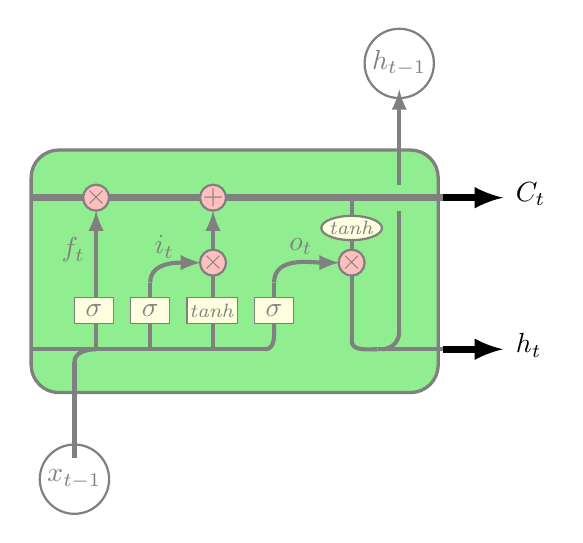
\begin{tikzpicture}[scale=1.1]

  % The grid
  % \draw[step=0.5, gray!40, very thin] (0,0) grid (8,4);

  % LSTM frame
  \def \yONE {0.5}
  \def \yTWO {3.3}
  \draw[rounded corners=10pt, very thick, gray,fill=LightGreen]  (1.5, 0.5) rectangle (6.2, 3.3);

  \def \sigmoidWidth  {0.45}
  \def \sigmoidInDist {0.2}
  \def \sigmoidHeight  {0.3}
  \def \yB  {1.3}
  \def \yD  {2.75}
  \def \shift {0.3}
  % First Sigmoid
  \draw[gray,fill=LightYellow] (2, \yB) rectangle (2+ \sigmoidWidth, \yB + \sigmoidHeight) node[pos=0.5] {$\sigma$};

  \def \r {.15cm}
  % The Upper times operator % first time from left
  \draw[thick, gray,fill=pink] (2.25, \yD) circle (\r) node {$\times$};

  % Second Sigmoid
  \def \xS {2.45 +\sigmoidInDist}
  \draw[gray,fill=LightYellow]  (\xS, \yB) rectangle (\xS +\sigmoidWidth, \yB + \sigmoidHeight) node[pos=0.5] {$\sigma$};

  % Square tanh
  \def \xSS {\xS +\sigmoidWidth + \sigmoidInDist}
  \draw[gray,fill=LightYellow]  (\xSS, \yB) 
  rectangle 
  (\xSS +\sigmoidWidth +0.13, \yB +\sigmoidHeight)
  node[pos=0.5] {\scriptsize \textit{tanh}};

  % Third Sigoid
  \def \xSSS {\xSS +\sigmoidWidth +0.13 +\sigmoidInDist}
  \draw[gray,fill=LightYellow]  (\xSSS, \yB) rectangle (\xSSS +\sigmoidWidth, \yB +\sigmoidHeight)
  node[pos=0.5] { $\sigma$};

  % Second times operator and add operator
  \def \xTimesB {3.6}
  \def \yC      {2}

  \draw[thick,gray,fill=pink] (\xTimesB, \yC) circle (\r) node {$\times$};
  %%%%% first line sectond operator +
  \draw[thick, gray,fill=pink] (\xTimesB, \yD) circle (\r) node {$+$};

  % Third times operator and its tanh
  \draw[thick,gray,fill=pink] (\xTimesB +1.3 +\shift, \yC) circle (\r) node {$\times$};
  \draw[thick,gray,fill=LightYellow] (\xTimesB +1.3 +\shift, \yC +.4)  
  ellipse (.35cm and .14cm) 
  node {\scriptsize \textit{tanh}};


  % LINES %%% Upper line from c_{t -1} till C_t
  %\draw[arrows=-latex, line width=2.5pt]  (0.85, \yD) -- (1.5, \yD) node[left, xshift=-.6cm, yshift=0.2cm] {$C_{t-1}$};
  \draw[line width=2.5pt, gray]  (1.5, \yD) -- (2.1, \yD);
  \draw[line width=2.5pt, gray]  (2.4, \yD) -- (3.46, \yD);
  \draw[line width=2.5pt,gray]  (3.75, \yD) -- (6.25 +0.2, \yD);

  \draw[arrows=-latex, line width=2.5pt]  (6.25, \yD) -- (6.75 +0.2, \yD)
  node[right, xshift=0.0cm, yshift=0.05cm] {$C_t$};

  %%%%first line from left from sigmoid ft till times input from C_{t-1}
  \draw[arrows=-latex, line width=1.5pt,gray]  (2.25, \yB +\sigmoidHeight) -- (2.25, 2.6)
  node[left, yshift=-0.5cm] {$f_t$};

  % Level B LINES
  \def \levelB {1}
  %\draw[arrows=-latex, line width=1.5pt,gray] (0.85, \levelB) -- (1.5, \levelB) node[left, xshift=-.6cm, yshift=0.2cm] {$h_{t-1}$};

  \draw[line width=1.5pt,gray] (1.5, \levelB) 
  --
  (4.2, \levelB);

  \def \xOfThirdSigmoid {\xSSS + \sigmoidWidth/2}
  %second line last angle connected to sigmoid 
  \draw[line width=1.5pt,gray] (4.2, \levelB) to[out=0,in=270] (\xOfThirdSigmoid, \yB);

  % Third Sigmoid up line
  % END (\xTimesB +1.3 - 0.19 , \yC)
  \draw[line width=1.5pt,gray] (\xOfThirdSigmoid, \yB + \sigmoidHeight) 
  --
  (\xOfThirdSigmoid, \yB + \sigmoidHeight + 0.17) ;

  \draw[arrows=-latex, line width=1.5pt,gray] (\xOfThirdSigmoid, \yB + \sigmoidHeight+0.17) 
  to[out=90, in=180] 
  (\xTimesB +1.3 -0.14 +\shift , \yC) 
  node [left, yshift=0.2cm, xshift=-0.2cm] {$o_t$};

  % tanh line
  \draw [line width=1.5pt,gray] (\xTimesB, \levelB)
  --
  (\xTimesB, \yB);

  \draw [line width=1.5pt,gray] (\xTimesB, \yB + \sigmoidHeight)
  --
  (\xTimesB, \yB + \sigmoidHeight +0.24);

  \draw [arrows=-latex, line width=1.5pt,gray] (\xTimesB, 2.15)
  --
  (\xTimesB, 2.6);

  \draw[line width=1.5pt,gray] (2.25, \levelB)
  --
  (2.25, \yB);
  
  \draw[line width=1.5pt,gray] (\xS +\sigmoidWidth/2, \levelB)
  --
  (\xS +\sigmoidWidth/2, \yB);

  \draw[line width=1.5pt,gray] (\xS +\sigmoidWidth/2, \yB +\sigmoidHeight)
  -- 
  (\xS +\sigmoidWidth/2, \yB +\sigmoidHeight + 0.17);

  \draw[arrows=-latex, line width=1.5pt,gray] (\xS +\sigmoidWidth/2, \yB + \sigmoidHeight+0.17) 
  to[out=90, in=180] 
  (\xTimesB-0.14, \yC)
  node [left, yshift=0.2cm, xshift=-0.2cm] {$i_t$};

  \def \bigR {0.25cm}
  \def \bigRTWO {0.4cm}
  \def \C    {1}
  \def \xBigCicleONE {2}
  \def \xBigCicleTWO {5.5 + 0.25}
  \draw[thick,gray] (\xBigCicleONE, \yONE - \C) circle (\bigRTWO) node {$x_{t-1}$};
  \draw[thick,gray] (\xBigCicleTWO, \yTWO + \C) circle (\bigRTWO) node {$h_{t-1}$};

  % LINE Circle ONE
  \draw[line width=1.5pt,gray] (\xBigCicleONE, \yONE -\C +0.25) 
  --
  (\xBigCicleONE, \yONE -\C +0.25 + 1.1);

  \draw[line width=1.5pt,gray] (\xBigCicleONE, \yONE -\C +0.25 + 1.1)
  to[out=90, in=180]
  (2.25, 1);

  % LINE third \times
  \draw[line width=1.5pt,gray] (\xTimesB +1.3 +\shift, 1.1)
  --
  (\xTimesB +1.3 +\shift, \yC - 0.15);

  \draw[line width=1.5pt,gray] (5.5, 1) 
  --
  (6.25 +0.2, 1);
  
  \draw[arrows=-latex,line width=2.5pt] (6.25, 1) 
  --
  (6.75 +0.2, 1)
  node[right, xshift=0.0cm, yshift=0.05cm,] {$h_t$};

%%% second line last angle connect the input with h_t output
  \draw[line width=1.5pt,gray] (\xTimesB +1.3 +\shift, 1.1)
  to[out=270, in=180]
  (5.5, 1);


  \draw[line width=1.5pt,gray] (\xTimesB +1.3 +\shift, 2.14)
  --
  (\xTimesB +1.3 +\shift, 2.26);


  \draw[line width=1.5pt,gray] (\xTimesB +1.3 +\shift, \yD)
  --
  (\xTimesB +1.3 +\shift, 2.54);


  \draw[line width=1.5pt,gray] (\xBigCicleTWO, \levelB +0.2)
  --
  (\xBigCicleTWO, 2.6);

%%%%% first horizontal line from the right angle connected to output ht
  \draw[line width=1.5pt,gray] (\xBigCicleTWO - 0.2, \levelB)
  to[out=0, in=270]
  (\xBigCicleTWO, \levelB +0.2);


  \draw[arrows=-latex, line width=1.5pt,gray]
  (\xBigCicleTWO, \yD +0.15)
  --
  (\xBigCicleTWO, 4);

\end{tikzpicture}


	\endminipage\hfill
	\minipage{0.33\textwidth}
	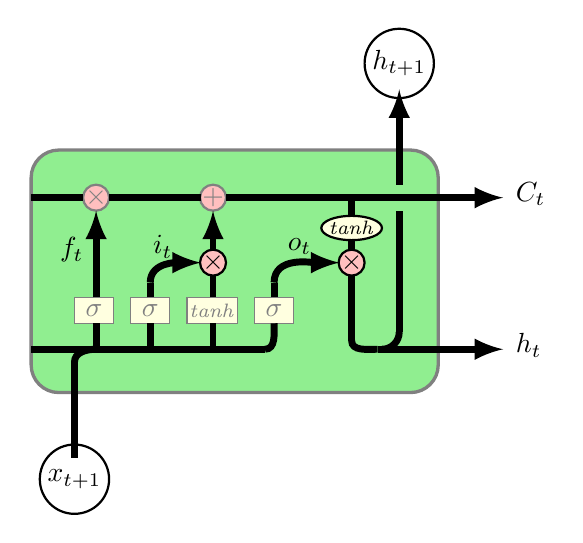
\begin{tikzpicture}[scale=1.1]

  % The grid
  % \draw[step=0.5, gray!40, very thin] (0,0) grid (8,4);

  % LSTM frame
  \def \yONE {0.5}
  \def \yTWO {3.3}
  \draw[rounded corners=10pt, very thick, gray,fill=LightGreen]  (1.5, 0.5) rectangle (6.2, 3.3);

  \def \sigmoidWidth  {0.45}
  \def \sigmoidInDist {0.2}
  \def \sigmoidHeight  {0.3}
  \def \yB  {1.3}
  \def \yD  {2.75}
  \def \shift {0.3}
  % First Sigmoid
  \draw[gray,fill=LightYellow] (2, \yB) rectangle (2+ \sigmoidWidth, \yB + \sigmoidHeight) node[pos=0.5] {$\sigma$};

  \def \r {.15cm}
  % The Upper times operator % first time from left
  \draw[thick, gray,fill=pink] (2.25, \yD) circle (\r) node {$\times$};

  % Second Sigmoid
  \def \xS {2.45 +\sigmoidInDist}
  \draw[gray,fill=LightYellow]  (\xS, \yB) rectangle (\xS +\sigmoidWidth, \yB + \sigmoidHeight) node[pos=0.5] {$\sigma$};

  % Square tanh
  \def \xSS {\xS +\sigmoidWidth + \sigmoidInDist}
  \draw[gray,fill=LightYellow]  (\xSS, \yB) 
  rectangle 
  (\xSS +\sigmoidWidth +0.13, \yB +\sigmoidHeight)
  node[pos=0.5] {\scriptsize \textit{tanh}};

  % Third Sigoid
  \def \xSSS {\xSS +\sigmoidWidth +0.13 +\sigmoidInDist}
  \draw[gray,fill=LightYellow]  (\xSSS, \yB) rectangle (\xSSS +\sigmoidWidth, \yB +\sigmoidHeight)
  node[pos=0.5] { $\sigma$};

  % Second times operator and add operator
  \def \xTimesB {3.6}
  \def \yC      {2}

  \draw[thick,fill=pink] (\xTimesB, \yC) circle (\r) node {$\times$};
  %%%%% first line sectond operator +
  \draw[thick, gray,fill=pink] (\xTimesB, \yD) circle (\r) node {$+$};

  % Third times operator and its tanh
  \draw[thick,fill=pink] (\xTimesB +1.3 +\shift, \yC) circle (\r) node {$\times$};
  \draw[thick,fill=LightYellow] (\xTimesB +1.3 +\shift, \yC +.4)  
  ellipse (.35cm and .14cm) 
  node {\scriptsize \textit{tanh}};


  % LINES %%% Upper line from c_{t -1} till C_t
  %\draw[arrows=-latex, line width=2.5pt]  (0.85, \yD) -- (1.5, \yD) node[left, xshift=-.6cm, yshift=0.2cm] {$C_{t-1}$};
  \draw[line width=2.5pt]  (1.5, \yD) -- (2.1, \yD);
  \draw[line width=2.5pt]  (2.4, \yD) -- (3.46, \yD);
  \draw[line width=2.5pt]  (3.75, \yD) -- (6.25 +0.2, \yD);

  \draw[arrows=-latex, line width=2.5pt]  (6.25, \yD) -- (6.75 +0.2, \yD)
  node[right, xshift=0.0cm, yshift=0.05cm] {$C_t$};

  %%%%first line from left from sigmoid ft till times input from C_{t-1}
  \draw[arrows=-latex, line width=2.5pt]  (2.25, \yB +\sigmoidHeight) -- (2.25, 2.6)
  node[left, yshift=-0.5cm] {$f_t$};

  % Level B LINES
  \def \levelB {1}
  %\draw[arrows=-latex, line width=2.5pt] (0.85, \levelB) -- (1.5, \levelB) node[left, xshift=-.6cm, yshift=0.2cm] {$h_{t-1}$};

  \draw[line width=2.5pt] (1.5, \levelB) 
  --
  (4.2, \levelB);

  \def \xOfThirdSigmoid {\xSSS + \sigmoidWidth/2}
  %second line last angle connected to sigmoid 
  \draw[line width=2.5pt] (4.2, \levelB) to[out=0,in=270] (\xOfThirdSigmoid, \yB);

  % Third Sigmoid up line
  % END (\xTimesB +1.3 - 0.19 , \yC)
  \draw[line width=2.5pt] (\xOfThirdSigmoid, \yB + \sigmoidHeight) 
  --
  (\xOfThirdSigmoid, \yB + \sigmoidHeight + 0.17) ;

  \draw[arrows=-latex, line width=2.5pt] (\xOfThirdSigmoid, \yB + \sigmoidHeight+0.17) 
  to[out=90, in=180] 
  (\xTimesB +1.3 -0.14 +\shift , \yC) 
  node [left, yshift=0.2cm, xshift=-0.2cm] {$o_t$};

  % tanh line
  \draw [line width=2.5pt] (\xTimesB, \levelB)
  --
  (\xTimesB, \yB);

  \draw [line width=2.5pt] (\xTimesB, \yB + \sigmoidHeight)
  --
  (\xTimesB, \yB + \sigmoidHeight +0.24);

  \draw [arrows=-latex, line width=2.5pt] (\xTimesB, 2.15)
  --
  (\xTimesB, 2.6);

  \draw[line width=2.5pt] (2.25, \levelB)
  --
  (2.25, \yB);
  
  \draw[line width=2.5pt] (\xS +\sigmoidWidth/2, \levelB)
  --
  (\xS +\sigmoidWidth/2, \yB);

  \draw[line width=2.5pt] (\xS +\sigmoidWidth/2, \yB +\sigmoidHeight)
  -- 
  (\xS +\sigmoidWidth/2, \yB +\sigmoidHeight + 0.17);

  \draw[arrows=-latex, line width=2.5pt] (\xS +\sigmoidWidth/2, \yB + \sigmoidHeight+0.17) 
  to[out=90, in=180] 
  (\xTimesB-0.14, \yC)
  node [left, yshift=0.2cm, xshift=-0.2cm] {$i_t$};

  \def \bigR {0.25cm}
  \def \bigRTWO {0.4cm}
  \def \C    {1}
  \def \xBigCicleONE {2}
  \def \xBigCicleTWO {5.5 + 0.25}
  \draw[thick] (\xBigCicleONE, \yONE - \C) circle (\bigRTWO) node {$x_{t+1}$};
  \draw[thick] (\xBigCicleTWO, \yTWO + \C) circle (\bigRTWO) node {$h_{t+1}$};

  % LINE Circle ONE
  \draw[line width=2.5pt] (\xBigCicleONE, \yONE -\C +0.25) 
  --
  (\xBigCicleONE, \yONE -\C +0.25 + 1.1);

  \draw[line width=2.5pt] (\xBigCicleONE, \yONE -\C +0.25 + 1.1)
  to[out=90, in=180]
  (2.25, 1);

  % LINE third \times
  \draw[line width=2.5pt] (\xTimesB +1.3 +\shift, 1.1)
  --
  (\xTimesB +1.3 +\shift, \yC - 0.15);

  \draw[line width=2.5pt] (5.5, 1) 
  --
  (6.25 +0.2, 1);
  
  \draw[arrows=-latex, line width=2.5pt] (6.25, 1) 
  --
  (6.75 +0.2, 1)
  node[right, xshift=0.0cm, yshift=0.05cm,] {$h_t$};

%%% second line last angle connect the input with h_t output
  \draw[line width=2.5pt] (\xTimesB +1.3 +\shift, 1.1)
  to[out=270, in=180]
  (5.5, 1);


  \draw[line width=2.5pt] (\xTimesB +1.3 +\shift, 2.14)
  --
  (\xTimesB +1.3 +\shift, 2.26);


  \draw[line width=2.5pt] (\xTimesB +1.3 +\shift, \yD)
  --
  (\xTimesB +1.3 +\shift, 2.54);


  \draw[line width=2.5pt] (\xBigCicleTWO, \levelB +0.2)
  --
  (\xBigCicleTWO, 2.6);

%%%%% first horizontal line from the right angle connected to output ht
  \draw[line width=2.5pt] (\xBigCicleTWO - 0.2, \levelB)
  to[out=0, in=270]
  (\xBigCicleTWO, \levelB +0.2);


  \draw[arrows=-latex, line width=2.5pt]
  (\xBigCicleTWO, \yD +0.15)
  --
  (\xBigCicleTWO, 4);

\end{tikzpicture}


	\endminipage\hfill
	\minipage{0.33\textwidth}%
	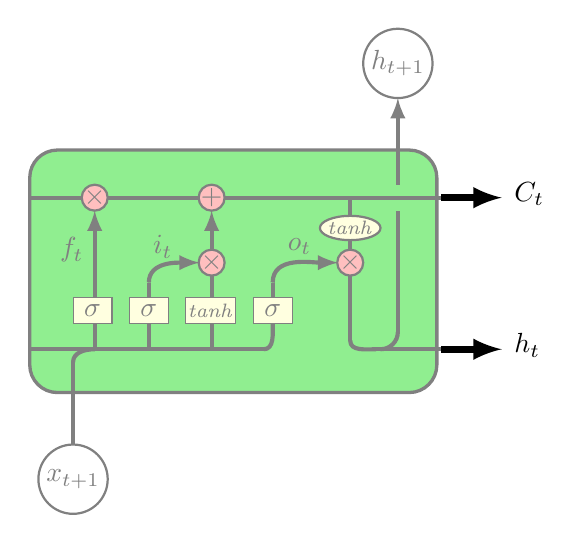
\begin{tikzpicture}[scale=1.1]

  % The grid
  % \draw[step=0.5, gray!40, very thin] (0,0) grid (8,4);

  % LSTM frame
  \def \yONE {0.5}
  \def \yTWO {3.3}
  \draw[rounded corners=10pt, very thick, gray,fill=LightGreen]  (1.5, 0.5) rectangle (6.2, 3.3);

  \def \sigmoidWidth  {0.45}
  \def \sigmoidInDist {0.2}
  \def \sigmoidHeight  {0.3}
  \def \yB  {1.3}
  \def \yD  {2.75}
  \def \shift {0.3}
  % First Sigmoid
  \draw[gray,fill=LightYellow] (2, \yB) rectangle (2+ \sigmoidWidth, \yB + \sigmoidHeight) node[pos=0.5] {$\sigma$};

  \def \r {.15cm}
  % The Upper times operator % first time from left
  \draw[thick, gray,fill=pink] (2.25, \yD) circle (\r) node {$\times$};

  % Second Sigmoid
  \def \xS {2.45 +\sigmoidInDist}
  \draw[gray,fill=LightYellow]  (\xS, \yB) rectangle (\xS +\sigmoidWidth, \yB + \sigmoidHeight) node[pos=0.5] {$\sigma$};

  % Square tanh
  \def \xSS {\xS +\sigmoidWidth + \sigmoidInDist}
  \draw[gray,fill=LightYellow]  (\xSS, \yB) 
  rectangle 
  (\xSS +\sigmoidWidth +0.13, \yB +\sigmoidHeight)
  node[pos=0.5] {\scriptsize \textit{tanh}};

  % Third Sigoid
  \def \xSSS {\xSS +\sigmoidWidth +0.13 +\sigmoidInDist}
  \draw[gray,fill=LightYellow]  (\xSSS, \yB) rectangle (\xSSS +\sigmoidWidth, \yB +\sigmoidHeight)
  node[pos=0.5] { $\sigma$};

  % Second times operator and add operator
  \def \xTimesB {3.6}
  \def \yC      {2}

  \draw[thick,gray,fill=pink] (\xTimesB, \yC) circle (\r) node {$\times$};
  %%%%% first line sectond operator +
  \draw[thick, gray,fill=pink] (\xTimesB, \yD) circle (\r) node {$+$};

  % Third times operator and its tanh
  \draw[thick,gray,fill=pink] (\xTimesB +1.3 +\shift, \yC) circle (\r) node {$\times$};
  \draw[thick,gray,fill=LightYellow] (\xTimesB +1.3 +\shift, \yC +.4)  
  ellipse (.35cm and .14cm) 
  node {\scriptsize \textit{tanh}};


  % LINES %%% Upper line from c_{t -1} till C_t
  %\draw[arrows=-latex, line width=2.5pt]  (0.85, \yD) -- (1.5, \yD) node[left, xshift=-.6cm, yshift=0.2cm] {$C_{t-1}$};
  \draw[line width=1.5pt,gray]  (1.5, \yD) -- (2.1, \yD);
  \draw[line width=1.5pt,gray]  (2.4, \yD) -- (3.46, \yD);
  \draw[line width=1.5pt,gray]  (3.75, \yD) -- (6.25 +0.2, \yD);

  \draw[arrows=-latex, line width=2.5pt]  (6.25, \yD) -- (6.75 +0.2, \yD)
  node[right, xshift=0.0cm, yshift=0.05cm] {$C_t$};

  %%%%first line from left from sigmoid ft till times input from C_{t-1}
  \draw[arrows=-latex, line width=1.5pt,gray]  (2.25, \yB +\sigmoidHeight) -- (2.25, 2.6)
  node[left, yshift=-0.5cm] {$f_t$};

  % Level B LINES
  \def \levelB {1}
  %\draw[arrows=-latex, line width=1.5pt,gray] (0.85, \levelB) -- (1.5, \levelB) node[left, xshift=-.6cm, yshift=0.2cm] {$h_{t-1}$};

  \draw[line width=1.5pt,gray] (1.5, \levelB) 
  --
  (4.2, \levelB);

  \def \xOfThirdSigmoid {\xSSS + \sigmoidWidth/2}
  %second line last angle connected to sigmoid 
  \draw[line width=1.5pt,gray] (4.2, \levelB) to[out=0,in=270] (\xOfThirdSigmoid, \yB);

  % Third Sigmoid up line
  % END (\xTimesB +1.3 - 0.19 , \yC)
  \draw[line width=1.5pt,gray] (\xOfThirdSigmoid, \yB + \sigmoidHeight) 
  --
  (\xOfThirdSigmoid, \yB + \sigmoidHeight + 0.17) ;

  \draw[arrows=-latex, line width=1.5pt,gray] (\xOfThirdSigmoid, \yB + \sigmoidHeight+0.17) 
  to[out=90, in=180] 
  (\xTimesB +1.3 -0.14 +\shift , \yC) 
  node [left, yshift=0.2cm, xshift=-0.2cm] {$o_t$};

  % tanh line
  \draw [line width=1.5pt,gray] (\xTimesB, \levelB)
  --
  (\xTimesB, \yB);

  \draw [line width=1.5pt,gray] (\xTimesB, \yB + \sigmoidHeight)
  --
  (\xTimesB, \yB + \sigmoidHeight +0.24);

  \draw [arrows=-latex, line width=1.5pt,gray] (\xTimesB, 2.15)
  --
  (\xTimesB, 2.6);

  \draw[line width=1.5pt,gray] (2.25, \levelB)
  --
  (2.25, \yB);
  
  \draw[line width=1.5pt,gray] (\xS +\sigmoidWidth/2, \levelB)
  --
  (\xS +\sigmoidWidth/2, \yB);

  \draw[line width=1.5pt,gray] (\xS +\sigmoidWidth/2, \yB +\sigmoidHeight)
  -- 
  (\xS +\sigmoidWidth/2, \yB +\sigmoidHeight + 0.17);

  \draw[arrows=-latex, line width=1.5pt,gray] (\xS +\sigmoidWidth/2, \yB + \sigmoidHeight+0.17) 
  to[out=90, in=180] 
  (\xTimesB-0.14, \yC)
  node [left, yshift=0.2cm, xshift=-0.2cm] {$i_t$};

  \def \bigR {0.25cm}
  \def \bigRTWO {0.4cm}
  \def \C    {1}
  \def \xBigCicleONE {2}
  \def \xBigCicleTWO {5.5 + 0.25}
  \draw[thick,gray] (\xBigCicleONE, \yONE - \C) circle (\bigRTWO) node {$x_{t+1}$};
  \draw[thick,gray] (\xBigCicleTWO, \yTWO + \C) circle (\bigRTWO) node {$h_{t+1}$};

  % LINE Circle ONE
  \draw[line width=1.5pt,gray] (\xBigCicleONE, \yONE -\C +0.4) 
  --
  (\xBigCicleONE, \yONE -\C +0.25 + 1.1);

  \draw[line width=1.5pt,gray] (\xBigCicleONE, \yONE -\C +0.25 + 1.1)
  to[out=90, in=180]
  (2.25, 1);

  % LINE third \times
  \draw[line width=1.5pt,gray] (\xTimesB +1.3 +\shift, 1.1)
  --
  (\xTimesB +1.3 +\shift, \yC - 0.15);

  \draw[line width=1.5pt,gray] (5.5, 1) 
  --
  (6.25 +0.2, 1);
  
  \draw[arrows=-latex,line width=2.5pt] (6.25, 1) 
  --
  (6.75 +0.2, 1)
  node[right, xshift=0.0cm, yshift=0.05cm,] {$h_t$};

%%% second line last angle connect the input with h_t output
  \draw[line width=1.5pt,gray] (\xTimesB +1.3 +\shift, 1.1)
  to[out=270, in=180]
  (5.5, 1);


  \draw[line width=1.5pt,gray] (\xTimesB +1.3 +\shift, 2.14)
  --
  (\xTimesB +1.3 +\shift, 2.26);


  \draw[line width=1.5pt,gray] (\xTimesB +1.3 +\shift, \yD)
  --
  (\xTimesB +1.3 +\shift, 2.54);


  \draw[line width=1.5pt,gray] (\xBigCicleTWO, \levelB +0.2)
  --
  (\xBigCicleTWO, 2.6);

%%%%% first horizontal line from the right angle connected to output ht
  \draw[line width=1.5pt,gray] (\xBigCicleTWO - 0.2, \levelB)
  to[out=0, in=270]
  (\xBigCicleTWO, \levelB +0.2);


  \draw[arrows=-latex, line width=1.5pt,gray]
  (\xBigCicleTWO, \yD +0.15)
  --
  (\xBigCicleTWO, 4-.1);

\end{tikzpicture}

	\endminipage
	\caption{The repeating module in an LSTM containing four interacting layers adapted from~\cite{colah}}~\label{Fig:LSTM_Cell_Chaining}
\end{figure}%

\subsubsection{LSTM Gate Mechanism}

The main component of LSTM is the cell state; this allows the information to pass through it unchanged. In figure~\ref{Fig:LSTM_Gate} the top line shows the information flow through the cell. The LSTM cell can add or remove information to the cell state using the Gating mechanism. 

Gates's idea is a methodology to manage how and which information passes or not. It controls information flow through the cell. It has three of these gates. They consist of a sigmoid neural network layer~\ref{Fig:LSTM_Cell_State} and a pointwise multiplication operation~\ref{Fig:LSTM_Gate}.

Sigmoid function output values range between zero and one. If the value is one, everything should pass, while if the value is zero nothing passes. Hence, the value output from the sigmoid function refers to the amount of each component should be passed.%

\subsubsection{How LSTM Works}

We have explained LSTM has three gates:

\begin{itemize}
 
\item \textbf{Forget Gate Layer} a Sigmoid layer Figure~\ref{Fig:LSTM-forget-gate} decides which information will be allowed to pass and which will not. It looks at $h_{t-1}$ and $x_t$, and calculates the output from Sigmoid function between zero and one. As explained, if one \textit{everything should pass}, while if zero \textit{nothing passes}. The value zero or one depends on the value of the cell state; if it includes a gender type and we need to predict the pronouns so, it will pass. Otherwise, it will ignore this state~\eqref{eq:lstm_gate}.%
\begin{equation}\label{eq:lstm_gate}
f_t = \sigma(W_f x_t + U_f h_{t-1} + b_t)
\end{equation}%

\item \textbf{Input Gate Layer} a combination between sigmoid layer which works to decide which values should be updated, and $\tanh$ layer creates a new vector of the new information $\tilde{C_t}$ which should be stored for the next state Figure~\ref{Fig:LSTM_Input_Gate}. The previous combination controls the update state as shown in Equation~\eqref{eq:input_gate}. This layer is used when we have new input information. For example, if we have a new subject named Elizabeth we need to store it for the next input. The next step is the pointwise multiplication and addition operations.%
\begin{subequations}\label{eq:input_gate}
\begin{align}
 i_t &= \sigma(W_i \dot[h_{t-1},x_t] + b_i)\\
\widetilde{C_t} &= \tanh(W_C\dot [h_{t-1},x_t]+ b_C)
\end{align}
\end{subequations}

\item \textbf{Multiplication and Addition operations} This step is to apply the actions recommended by the previous gates as shown in Equation~\eqref{eq:multiplication_gate}. This step is the actions applying the forgetting of the old information and addition of the new information, as decided in the previous steps. Regarding the upper line in Figure~\ref{Fig:LSTM_Pointwise_Operations}, there are two operations:
\begin{enumerate}
\item Multiplication Operation: This operation applies the forget gate step by multiplying the old state $\tilde{C}_{t-1} $ by the $f_t$.
\item Addition Operation: This operation will add the output from the previous multiplication with the new input information scaled by how much we need to update each state value $i_t \times \tilde{C_t}$
\end{enumerate}%
 
\begin{equation}\label{eq:multiplication_gate}
C_t = f_t \circ c_{t-1} + i_t \circ \widetilde{C_t}
\end{equation}
   
  \item \textbf{Output Gate} This gate is a combination of sigmoid layer and $\tanh$ layer. Sigmoid layer decides the information which should be output. Then the output of the  sigmoid function will be multiplied by the output of the $\tanh$ layer of the cell state. This $\tanh$ will make the values between -1 and 1. The output of the multiplication of sigmoid and $\tanh$ will be the final output, as shown in Equation~\eqref{eq:output_gate}. In practice, this gate responsible for deciding which information should be the output. For example, if it saw a subject such as Elizabeth, it might want to output a verb to be relevant to her as a singular.%
\begin{subequations}\label{eq:output_gate}
\begin{align}
o_t &= \sigma(W_o x_t + U_o h_{t-1} + b_o),\\
h_t &= o_t \circ \tanh(C_t)
\end{align}
\end{subequations}%
\end{itemize}

We have explained the normal LSTM. We also need to mention that much research proposes different modifications of the normal LSTM type. We do not explain all the types, but we give a small overview of one of these modifications named Gated Recurrent Unit (GRU) in the next part.

\subsubsection{Gated Recurrent Units (GRUs)}

In RNN, Gated recurrent units (GRUs) are a gating mechanism, introduced in 2014 by Kyunghyun Cho et al.~\cite{Cho_et_al}. They work to overcome the problem for long-term dependencies. It also aims to solve the vanishing gradient problem from Basic RNNs.It proposed a new architecture Figure~\ref{Fig:GRU} similar to the LSTM but with some major variants as below:

\begin{itemize}
\item It combines the forget gate and input gates into a single gate named “update gate and reset gate.”
\item The GRU unit controls the flow of information without having to use a memory unit. It simply exposes the full hidden content without any control.
\item It also merges the cell state and hidden state.
\end{itemize}%

The result of this modifications is that GRUs are simpler and easier for modifications in design. GRUs trains faster and in some cases performs better than LSTMs on less training data, mainly in language modelling. However, LSTMs have some benefits over GRUs, with longer sequences in tasks requiring modelling long-distance relations.
\begin{figure}[!ht]
	\centering
	\subfigure[Top line is the medium for information flow]
	{
		\label{Fig:LSTM_Cell_State}
		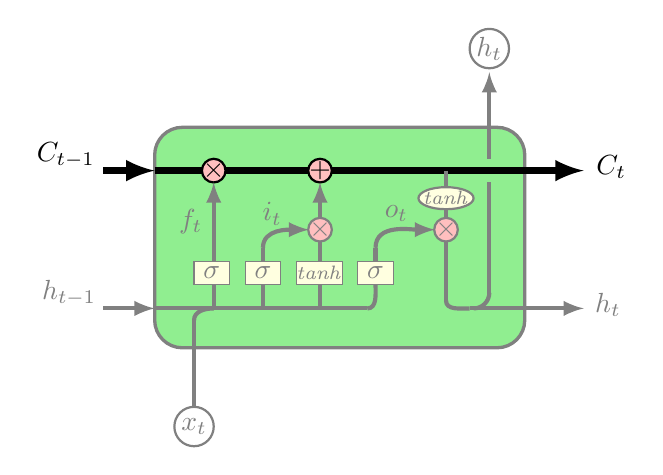
\begin{tikzpicture}

  % The grid
  % \draw[step=0.5, gray!40, very thin] (0,0) grid (8,4);

  % LSTM frame
  \def \yONE {0.5}
  \def \yTWO {3.3}
  \draw[rounded corners=10pt, very thick, gray,fill=LightGreen]  (1.5, 0.5) rectangle (6.2, 3.3);

  \def \sigmoidWidth  {0.45}
  \def \sigmoidInDist {0.2}
  \def \sigmoidHeight  {0.3}
  \def \yB  {1.3}
  \def \yD  {2.75}
  \def \shift {0.3}
  % First Sigmoid
  \draw[gray,fill=LightYellow] (2, \yB) rectangle (2+ \sigmoidWidth, \yB + \sigmoidHeight) node[pos=0.5] {$\sigma$};

  \def \r {.15cm}
  % The Upper times operator % first time from left
  \draw[thick,fill=pink] (2.25, \yD) circle (\r) node {$\times$};

  % Second Sigmoid
  \def \xS {2.45 +\sigmoidInDist}
  \draw[gray,fill=LightYellow]  (\xS, \yB) rectangle (\xS +\sigmoidWidth, \yB + \sigmoidHeight) node[pos=0.5] {$\sigma$};

  % Square tanh
  \def \xSS {\xS +\sigmoidWidth + \sigmoidInDist}
  \draw[gray,fill=LightYellow]  (\xSS, \yB) 
  rectangle 
  (\xSS +\sigmoidWidth +0.13, \yB +\sigmoidHeight)
  node[pos=0.5] {\scriptsize \textit{tanh}};

  % Third Sigoid
  \def \xSSS {\xSS +\sigmoidWidth +0.13 +\sigmoidInDist}
  \draw[gray,fill=LightYellow]  (\xSSS, \yB) rectangle (\xSSS +\sigmoidWidth, \yB +\sigmoidHeight)
  node[pos=0.5] { $\sigma$};

  % Second times operator and add operator
  \def \xTimesB {3.6}
  \def \yC      {2}

  \draw[thick,gray,fill=pink] (\xTimesB, \yC) circle (\r) node {$\times$};
  %%%%% first line sectond operator +
  \draw[thick,fill=pink] (\xTimesB, \yD) circle (\r) node {$+$};

  % Third times operator and its tanh
  \draw[thick,gray,fill=pink] (\xTimesB +1.3 +\shift, \yC) circle (\r) node {$\times$};
  \draw[thick,gray,fill=LightYellow] (\xTimesB +1.3 +\shift, \yC +.4)  
  ellipse (.35cm and .14cm) 
  node {\scriptsize \textit{tanh}};


  % LINES %%% Upper line from c_{t -1} till C_t
  \draw[arrows=-latex, line width=2.5pt]  (0.85, \yD) -- (1.5, \yD) node[left, xshift=-.6cm, yshift=0.2cm] {$C_{t-1}$};
  \draw[line width=2.5pt]  (1.5, \yD) -- (2.1, \yD);
  \draw[line width=2.5pt]  (2.4, \yD) -- (3.46, \yD);
  \draw[arrows=-latex, line width=2.5pt]  (3.75, \yD) -- (6.75 +0.2, \yD)
  node[right, xshift=0.0cm, yshift=0.05cm] {$C_t$};

  %%%%first line from left from sigmoid ft till times input from C_{t-1}
  \draw[arrows=-latex, line width=1.5pt,gray]  (2.25, \yB +\sigmoidHeight) -- (2.25, 2.6)
  node[left, yshift=-0.5cm] {$f_t$};

  % Level B LINES
  \def \levelB {1}
  \draw[arrows=-latex, line width=1.5pt,gray] (0.85, \levelB) -- (1.5, \levelB)
  node[left, xshift=-.6cm, yshift=0.2cm] {$h_{t-1}$};

  \draw[line width=1.5pt,gray] (1.5, \levelB) 
  --
  (4.2, \levelB);

  \def \xOfThirdSigmoid {\xSSS + \sigmoidWidth/2}
  %second line last angle connected to sigmoid 
  \draw[line width=1.5pt,gray] (4.2, \levelB) to[out=0,in=270] (\xOfThirdSigmoid, \yB);

  % Third Sigmoid up line
  % END (\xTimesB +1.3 - 0.19 , \yC)
  \draw[line width=1.5pt,gray] (\xOfThirdSigmoid, \yB + \sigmoidHeight) 
  --
  (\xOfThirdSigmoid, \yB + \sigmoidHeight + 0.17) ;

  \draw[arrows=-latex, line width=1.5pt,gray] (\xOfThirdSigmoid, \yB + \sigmoidHeight+0.17) 
  to[out=90, in=180] 
  (\xTimesB +1.3 -0.14 +\shift , \yC) 
  node [left, yshift=0.2cm, xshift=-0.2cm] {$o_t$};

  % tanh line
  \draw [line width=1.5pt,gray] (\xTimesB, \levelB)
  --
  (\xTimesB, \yB);

  \draw [line width=1.5pt,gray] (\xTimesB, \yB + \sigmoidHeight)
  --
  (\xTimesB, \yB + \sigmoidHeight +0.24);

  \draw [arrows=-latex, line width=1.5pt,gray] (\xTimesB, 2.15)
  --
  (\xTimesB, 2.6);

  \draw[line width=1.5pt,gray] (2.25, \levelB)
  --
  (2.25, \yB);
  
  \draw[line width=1.5pt,gray] (\xS +\sigmoidWidth/2, \levelB)
  --
  (\xS +\sigmoidWidth/2, \yB);

  \draw[line width=1.5pt,gray] (\xS +\sigmoidWidth/2, \yB +\sigmoidHeight)
  -- 
  (\xS +\sigmoidWidth/2, \yB +\sigmoidHeight + 0.17);

  \draw[arrows=-latex, line width=1.5pt,gray] (\xS +\sigmoidWidth/2, \yB + \sigmoidHeight+0.17) 
  to[out=90, in=180] 
  (\xTimesB-0.14, \yC)
  node [left, yshift=0.2cm, xshift=-0.2cm] {$i_t$};

  \def \bigR {0.25cm}
  \def \C    {1}
  \def \xBigCicleONE {2}
  \def \xBigCicleTWO {5.5 + 0.25}
  \draw[thick,gray] (\xBigCicleONE, \yONE - \C) circle (\bigR) node {$x_t$};
  \draw[thick,gray] (\xBigCicleTWO, \yTWO + \C) circle (\bigR) node {$h_t$};

  % LINE Circle ONE
  \draw[line width=1.5pt,gray] (\xBigCicleONE, \yONE -\C +0.25) 
  --
  (\xBigCicleONE, \yONE -\C +0.25 + 1.1);

  \draw[line width=1.5pt,gray] (\xBigCicleONE, \yONE -\C +0.25 + 1.1)
  to[out=90, in=180]
  (2.25, 1);

  % LINE third \times
  \draw[line width=1.5pt,gray] (\xTimesB +1.3 +\shift, 1.1)
  --
  (\xTimesB +1.3 +\shift, \yC - 0.15);

  \draw[arrows=-latex, line width=1.5pt,gray] (5.5, 1) 
  --
  (6.75 +0.2, 1)
  node[right, xshift=0.0cm, yshift=0.05cm,] {$h_t$};

%%% second line last angle connect the input with h_t output
  \draw[line width=1.5pt,gray] (\xTimesB +1.3 +\shift, 1.1)
  to[out=270, in=180]
  (5.5, 1);


  \draw[line width=1.5pt,gray] (\xTimesB +1.3 +\shift, 2.14)
  --
  (\xTimesB +1.3 +\shift, 2.26);


  \draw[line width=1.5pt,gray] (\xTimesB +1.3 +\shift, \yD)
  --
  (\xTimesB +1.3 +\shift, 2.54);


  \draw[line width=1.5pt,gray] (\xBigCicleTWO, \levelB +0.2)
  --
  (\xBigCicleTWO, 2.6);

%%%%% first horizontal line from the right angle connected to output ht
  \draw[line width=1.5pt,gray] (\xBigCicleTWO - 0.2, \levelB)
  to[out=0, in=270]
  (\xBigCicleTWO, \levelB +0.2);


  \draw[arrows=-latex, line width=1.5pt,gray]
  (\xBigCicleTWO, \yD +0.15)
  --
  (\xBigCicleTWO, 4);

\end{tikzpicture}

	}
	\subfigure[Pointwise Multiplication Operation]
	{
		\label{Fig:LSTM_Gate}
		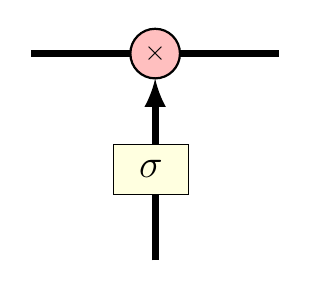
\begin{tikzpicture}[scale=2.1]

% The grid
% \draw[step=0.5, gray!40, very thin] (0,0) grid (8,4);

% LSTM frame
\def \yONE {0.5}
\def \yTWO {3.3}
\def \sigmoidWidth  {0.45}
\def \sigmoidInDist {0.2}
\def \sigmoidHeight  {0.3}
\def \yB  {1.3}
\def \yD  {2.75}
\def \shift {0.3}
% First Sigmoid
\draw[fill=LightYellow] (2, \yB+.6) rectangle (2+ \sigmoidWidth, \yB +.6+ \sigmoidHeight) node[pos=0.5] {\Large$\sigma$};

\def \r {.15cm}
% The Upper times operator % first time from left
\draw[thick, fill=pink] (2.25, \yD) circle (\r) node {$\times$};

\draw[line width=2.5pt]  (1.5, \yD) -- (2.1, \yD);
\draw[line width=2.5pt]  (2.4, \yD) -- (3, \yD);


%%%%first line from left from sigmoid ft till times input from C_{t-1}
\draw[line width=2.5pt]  (2.25, \yB +.2) -- (2.25, \yB+.3 +\sigmoidHeight);
\draw[arrows=-latex, line width=2.5pt]  (2.25, \yB+.3 +\sigmoidHeight+\sigmoidHeight)--(2.25, \yD-.15);

\end{tikzpicture}
	}
	\subfigure[LSTM sigmoid forget gate]
	{
		\label{Fig:LSTM-forget-gate}
		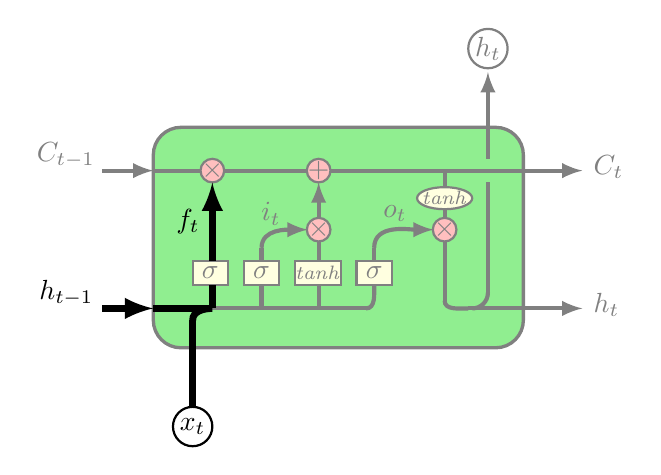
\begin{tikzpicture}
  % The grid
  % \draw[step=0.5, gray!40, very thin] (0,0) grid (8,4);

  % LSTM frame
  \def \yONE {0.5}
  \def \yTWO {3.3}
  \draw[rounded corners=10pt, very thick, gray,fill=LightGreen]  (1.5, 0.5) rectangle (6.2, 3.3);

  \def \sigmoidWidth  {0.45}
  \def \sigmoidInDist {0.2}
  \def \sigmoidHeight  {0.3}
  \def \yB  {1.3}
  \def \yD  {2.75}
  \def \shift {0.3}
  % First Sigmoid
  \draw[thick,gray,fill=LightYellow] (2, \yB) rectangle (2+ \sigmoidWidth, \yB + \sigmoidHeight) node[pos=0.5] {$\sigma$};

  \def \r {.15cm}
  % The Upper times operator % first time from left
  \draw[thick,gray,fill=pink] (2.25, \yD) circle (\r) node {$\times$};

  % Second Sigmoid
  \def \xS {2.45 +\sigmoidInDist}
  \draw[thick,gray,fill=LightYellow]  (\xS, \yB) rectangle (\xS +\sigmoidWidth, \yB + \sigmoidHeight) node[pos=0.5] {$\sigma$};

  % Square tanh
  \def \xSS {\xS +\sigmoidWidth + \sigmoidInDist}
  \draw[thick,gray,fill=LightYellow]  (\xSS, \yB) 
  rectangle 
  (\xSS +\sigmoidWidth +0.13, \yB +\sigmoidHeight)
  node[pos=0.5] {\scriptsize \textit{tanh}};

  % Third Sigoid
  \def \xSSS {\xSS +\sigmoidWidth +0.13 +\sigmoidInDist}
  \draw[gray,thick,fill=LightYellow]  (\xSSS, \yB) rectangle (\xSSS +\sigmoidWidth, \yB +\sigmoidHeight)
  node[pos=0.5] { $\sigma$};

  % Second times operator and add operator
  \def \xTimesB {3.6}
  \def \yC      {2}

  \draw[thick,gray,fill=pink] (\xTimesB, \yC) circle (\r) node {$\times$};
  
  %%%%% **first line sectond operator +
  \draw[thick,gray,fill=pink] (\xTimesB, \yD) circle (\r) node {$+$};

  % Third times operator and its tanh
  \draw[thick,gray,fill=pink] (\xTimesB +1.3 +\shift, \yC) circle (\r) node {$\times$};
  \draw[thick,gray,fill=LightYellow] (\xTimesB +1.3 +\shift, \yC +.4)  
  ellipse (.35cm and .14cm) 
  node {\scriptsize \textit{tanh}};


  % LINES %%% Upper line from c_{t -1} till C_t
  \draw[arrows=-latex, line width=1.5pt,gray]  (0.85, \yD) -- (1.5, \yD) node[left, xshift=-.6cm, yshift=0.2cm] {$C_{t-1}$};
  \draw[line width=1.5pt,gray]  (1.5, \yD) -- (2.1, \yD);
  \draw[line width=1.5pt,gray]  (2.4, \yD) -- (3.46, \yD);
  \draw[arrows=-latex, line width=1.5pt,gray]  (3.75, \yD) -- (6.75 +0.2, \yD)
  node[right, xshift=0.0cm, yshift=0.05cm] {$C_t$};

  %%%%first line from left from sigmoid ft till times input from C_{t-1}
  \draw[arrows=-latex, line width=2.5pt]  (2.25, \yB +\sigmoidHeight) -- (2.25, 2.6)
  node[left, yshift=-0.5cm] {$f_t$};

  % Level B LINES
  \def \levelB {1}
  %input h_{t-1} line
  \draw[arrows=-latex, line width=2.5pt] (0.85, \levelB) -- (1.5, \levelB)
  node[left, xshift=-.6cm, yshift=0.2cm] {$h_{t-1}$};

%level B line base between input h_{t-1} and first sigmoid
  \draw[line width=2.5pt] (1.5, \levelB) 
  --
  (2.25, \levelB);
  
  %level B line base between  first sigmoid and third sigmoid angle
   \draw[line width=1.5pt,gray] (2.25, \levelB) 
  --
  (4.2, \levelB);

  \def \xOfThirdSigmoid {\xSSS + \sigmoidWidth/2}
  %second line last angle connected to sigmoid 
  \draw[line width=1.5pt,gray] (4.2, \levelB) to[out=0,in=270] (\xOfThirdSigmoid, \yB);

  % Third Sigmoid up line
  % END (\xTimesB +1.3 - 0.19 , \yC)
  \draw[line width=1.5pt,gray] (\xOfThirdSigmoid, \yB + \sigmoidHeight) 
  --
  (\xOfThirdSigmoid, \yB + \sigmoidHeight + 0.17) ;

  \draw[arrows=-latex, line width=1.5pt,gray] (\xOfThirdSigmoid, \yB + \sigmoidHeight+0.17) 
  to[out=90, in=180] 
  (\xTimesB +1.3 -0.14 +\shift , \yC) 
  node [left, yshift=0.2cm, xshift=-0.2cm] {$o_t$};

  % tanh line
  \draw [line width=1.5pt,gray] (\xTimesB, \levelB)
  --
  (\xTimesB, \yB);

%line between first tanh from left and x
  \draw [line width=1.5pt,gray] (\xTimesB, \yB + \sigmoidHeight)
  --
  (\xTimesB, \yB + \sigmoidHeight +0.24);

%line between x and + upper first tanh from left
  \draw [arrows=-latex, line width=1.5pt,gray] (\xTimesB, 2.15)
  --
  (\xTimesB, 2.6);

%line between level B and first sigmoid
  \draw[line width=2.5pt] (2.25, \levelB)
  --
  (2.25, \yB);
  
  % line between level B and second sigmoid
  \draw[line width=1.5pt,gray] (\xS +\sigmoidWidth/2, \levelB)
  --
  (\xS +\sigmoidWidth/2, \yB);

% line angle between sgima and x midlle line
  \draw[line width=1.5pt,gray] (\xS +\sigmoidWidth/2, \yB +\sigmoidHeight)
  -- 
  (\xS +\sigmoidWidth/2, \yB +\sigmoidHeight + 0.17);

  %% angle between sgima and x midlle line
  \draw[arrows=-latex, line width=1.5pt,gray] (\xS +\sigmoidWidth/2, \yB + \sigmoidHeight+0.17) 
  to[out=90, in=180] 
  (\xTimesB-0.14, \yC)
  node [left, yshift=0.2cm, xshift=-0.2cm] {$i_t$};

  \def \bigR {0.25cm}
  \def \C    {1}
  \def \xBigCicleONE {2}
  \def \xBigCicleTWO {5.5 + 0.25}
  \draw[thick] (\xBigCicleONE, \yONE - \C) circle (\bigR) node {$x_t$};
  \draw[thick,gray] (\xBigCicleTWO, \yTWO + \C) circle (\bigR) node {$h_t$};

  % LINE Circle ONE from xt to line B
  \draw[line width=2.5pt] (\xBigCicleONE, \yONE -\C +0.25) 
  --
  (\xBigCicleONE, \yONE -\C +0.25 + 1.1);

%% angle from the x_t to sigma ifrst angle from the left down
  \draw[line width=2.5pt] (\xBigCicleONE, \yONE -\C +0.25 + 1.1)
  to[out=90, in=180]
  (2.25, 1);

  % LINE third \times
  \draw[line width=1.5pt,gray] (\xTimesB +1.3 +\shift, 1.1)
  --
  (\xTimesB +1.3 +\shift, \yC - 0.15);

  \draw[arrows=-latex, line width=1.5pt,gray] (5.5, 1) 
  --
  (6.75 +0.2, 1)
  node[right, xshift=0.0cm, yshift=0.05cm,] {$h_t$};

%%% second line last angle connect the input with h_t output
  \draw[line width=1.5pt,gray] (\xTimesB +1.3 +\shift, 1.1)
  to[out=270, in=180]
  (5.5, 1);


  \draw[line width=1.5pt,gray] (\xTimesB +1.3 +\shift, 2.14)
  --
  (\xTimesB +1.3 +\shift, 2.26);


  \draw[line width=1.5pt,gray] (\xTimesB +1.3 +\shift, \yD)
  --
  (\xTimesB +1.3 +\shift, 2.54);


  \draw[line width=1.5pt,gray] (\xBigCicleTWO, \levelB +0.2)
  --
  (\xBigCicleTWO, 2.6);

%%%%% first horizontal line from the right angle connected to output ht
  \draw[line width=1.5pt,gray] (\xBigCicleTWO - 0.2, \levelB)
  to[out=0, in=270]
  (\xBigCicleTWO, \levelB +0.2);


  \draw[arrows=-latex, line width=1.5pt,gray]
  (\xBigCicleTWO, \yD +0.15)
  --
  (\xBigCicleTWO, 4);

\end{tikzpicture}

	}
	\subfigure[LSTM Input gate]
	{
		\label{Fig:LSTM_Input_Gate}
		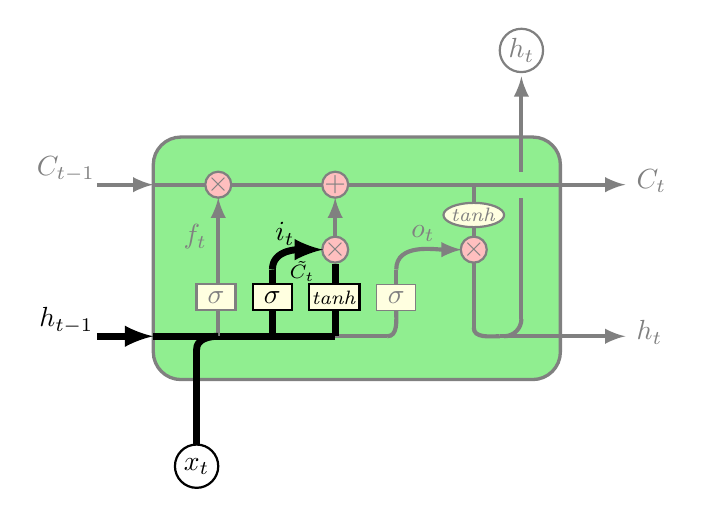
\begin{tikzpicture}[scale=1.1]

  % The grid
  % \draw[step=0.5, gray!40, very thin] (0,0) grid (8,4);

  % LSTM frame
  \def \yONE {0.5}
  \def \yTWO {3.3}
  \draw[rounded corners=10pt, very thick, gray,fill=LightGreen]  (1.5, 0.5) rectangle (6.2, 3.3);

  \def \sigmoidWidth  {0.45}
  \def \sigmoidInDist {0.2}
  \def \sigmoidHeight  {0.3}
  \def \yB  {1.3}
  \def \yD  {2.75}
  \def \shift {0.3}
  % First Sigmoid
  \draw[thick,gray,fill=LightYellow] (2, \yB) rectangle (2+ \sigmoidWidth, \yB + \sigmoidHeight) node[pos=0.5] {$\sigma$};

  \def \r {.15cm}
  % The Upper times operator % first time from left
  \draw[thick,gray,fill=pink] (2.25, \yD) circle (\r) node {$\times$};

  % Second Sigmoid
  \def \xS {2.45 +\sigmoidInDist}
  \draw[thick,,fill=LightYellow]  (\xS, \yB) rectangle (\xS +\sigmoidWidth, \yB + \sigmoidHeight) node[pos=0.5] {$\sigma$};

  % Square tanh
  \def \xSS {\xS +\sigmoidWidth + \sigmoidInDist}
  \draw[thick,,fill=LightYellow]  (\xSS, \yB) 
  rectangle 
  (\xSS +\sigmoidWidth +0.13, \yB +\sigmoidHeight)
  node[pos=0.5] {\scriptsize \textit{tanh}};

  % Third Sigoid
  \def \xSSS {\xSS +\sigmoidWidth +0.13 +\sigmoidInDist}
  \draw[gray,fill=LightYellow]  (\xSSS, \yB) rectangle (\xSSS +\sigmoidWidth, \yB +\sigmoidHeight)
  node[pos=0.5] { $\sigma$};

  % Second times operator and add operator
  \def \xTimesB {3.6}
  \def \yC      {2}

  \draw[thick,gray,fill=pink] (\xTimesB, \yC) circle (\r) node {$\times$};
  
  %%%%% **first line sectond operator +
  \draw[thick,gray,fill=pink] (\xTimesB, \yD) circle (\r) node {$+$};

  % Third times operator and its tanh
  \draw[thick,gray,fill=pink] (\xTimesB +1.3 +\shift, \yC) circle (\r) node {$\times$};
  \draw[thick,gray,fill=LightYellow] (\xTimesB +1.3 +\shift, \yC +.4)  
  ellipse (.35cm and .14cm) 
  node {\scriptsize \textit{tanh}};


  % LINES %%% Upper line from c_{t -1} till C_t
  \draw[arrows=-latex, line width=1.5pt,gray]  (0.85, \yD) -- (1.5, \yD) node[left, xshift=-.6cm, yshift=0.2cm] {$C_{t-1}$};
  \draw[line width=1.5pt,gray]  (1.5, \yD) -- (2.1, \yD);
  \draw[line width=1.5pt,gray]  (2.4, \yD) -- (3.46, \yD);
  \draw[arrows=-latex, line width=1.5pt,gray]  (3.75, \yD) -- (6.75 +0.2, \yD)
  node[right, xshift=0.0cm, yshift=0.05cm] {$C_t$};

  %%%%first line from left from sigmoid ft till times input from C_{t-1}
  \draw[arrows=-latex, line width=1.5pt,gray]  (2.25, \yB +\sigmoidHeight) -- (2.25, 2.6)
  node[left, yshift=-0.5cm] {$f_t$};

  % Level B LINES
  \def \levelB {1}
  %input h_{t-1} line
  \draw[arrows=-latex, line width=2.5pt] (0.85, \levelB) -- (1.5, \levelB)
  node[left, xshift=-.6cm, yshift=0.2cm] {$h_{t-1}$};

%level B line base between input h_{t-1} and first sigmoid
  \draw[line width=2.5pt] (1.5, \levelB) 
  --
  (2.25, \levelB);
  
  %level B line base between  first sigmoid and tanh
   \draw[line width=2.5pt] (2.25, \levelB) 
  --
  (3.6, \levelB);
  
  %level B line base between  tanh and tanh angle
  \draw[line width=1.5pt,gray] (3.6, \levelB) 
  --
  (4.2, \levelB);

  \def \xOfThirdSigmoid {\xSSS + \sigmoidWidth/2}
  %second line last angle connected to sigmoid 
  \draw[line width=1.5pt,gray] (4.2, \levelB) to[out=0,in=270] (\xOfThirdSigmoid, \yB);

  % Third Sigmoid up line
  % END (\xTimesB +1.3 - 0.19 , \yC)
  \draw[line width=1.5pt,gray] (\xOfThirdSigmoid, \yB + \sigmoidHeight) 
  --
  (\xOfThirdSigmoid, \yB + \sigmoidHeight + 0.17) ;

  \draw[arrows=-latex, line width=1.5pt,gray] (\xOfThirdSigmoid, \yB + \sigmoidHeight+0.17) 
  to[out=90, in=180] 
  (\xTimesB +1.3 -0.14 +\shift , \yC) 
  node [left, yshift=0.2cm, xshift=-0.2cm] {$o_t$};

  % tanh line
  \draw [line width=2.5pt] (\xTimesB, \levelB)
  --
  (\xTimesB, \yB);

%line between first tanh from left and x %%%%
  \draw [line width=2.5pt] (\xTimesB, \yB + \sigmoidHeight)
  --
  (\xTimesB, \yB + \sigmoidHeight +0.24)
  node [left, yshift=-0.1cm, xshift=-0.1cm] {\scriptsize$\tilde{C_t}$};

%line between x and + upper first tanh from left
  \draw [arrows=-latex, line width=1.5pt,gray] (\xTimesB, 2.15)
  --
  (\xTimesB, 2.6);

%line between level B and first sigmoid
  \draw[line width=1.5pt,gray] (2.25, \levelB)
  --
  (2.25, \yB);
  
  % line between level B and second sigmoid
  \draw[line width=2.5pt] (\xS +\sigmoidWidth/2, \levelB)
  --
  (\xS +\sigmoidWidth/2, \yB);

% line angle between sgima and x midlle line
  \draw[line width=2.5pt] (\xS +\sigmoidWidth/2, \yB +\sigmoidHeight)
  -- 
  (\xS +\sigmoidWidth/2, \yB +\sigmoidHeight + 0.17);

  %% angle between sgima and x midlle line i_t
  \draw[arrows=-latex, line width=2.5pt] (\xS +\sigmoidWidth/2, \yB + \sigmoidHeight+0.17) 
  to[out=90, in=180] 
  (\xTimesB-0.14, \yC)
  node [left, yshift=0.2cm, xshift=-0.2cm] {$i_t$};

  \def \bigR {0.25cm}
  \def \C    {1}
  \def \xBigCicleONE {2}
  \def \xBigCicleTWO {5.5 + 0.25}
  \draw[thick] (\xBigCicleONE, \yONE - \C) circle (\bigR) node {$x_t$};
  \draw[thick,gray] (\xBigCicleTWO, \yTWO + \C) circle (\bigR) node {$h_t$};

  % LINE Circle ONE from xt to line B
  \draw[line width=2.5pt] (\xBigCicleONE, \yONE -\C +0.25) 
  --
  (\xBigCicleONE, \yONE -\C +0.25 + 1.1);

%% angle from the x_t to sigma ifrst angle from the left down
  \draw[line width=2.5pt] (\xBigCicleONE, \yONE -\C +0.25 + 1.1)
  to[out=90, in=180]
  (2.25, 1);

  % LINE third \times betweem line B and times circle 
  \draw[line width=1.5pt,gray] (\xTimesB +1.3 +\shift, 1.1)
  --
  (\xTimesB +1.3 +\shift, \yC - 0.15);

  \draw[arrows=-latex, line width=1.5pt,gray] (5.5, 1) 
  --
  (6.75 +0.2, 1)
  node[right, xshift=0.0cm, yshift=0.05cm,] {$h_t$};

%%% second line last angle connect the input with h_t output
  \draw[line width=1.5pt,gray] (\xTimesB +1.3 +\shift, 1.1)
  to[out=270, in=180]
  (5.5, 1);


%%% line between times and tanh (last tanh h on the right alone)
  \draw[line width=1.5pt,gray] (\xTimesB +1.3 +\shift, 2.14)
  --
  (\xTimesB +1.3 +\shift, 2.26);

%%%%% Line between tanh and Line level A 
  \draw[line width=1.5pt,gray] (\xTimesB +1.3 +\shift, \yD)
  --
  (\xTimesB +1.3 +\shift, 2.54);

%%%%% first horizontal line from the right angle connected to the line which connect to output ht
  \draw[line width=1.5pt,gray] (\xBigCicleTWO, \levelB +0.2)
  --
  (\xBigCicleTWO, 2.6);

%%%%% first horizontal line from the right angle connected to output ht
  \draw[line width=1.5pt,gray] (\xBigCicleTWO - 0.2, \levelB)
  to[out=0, in=270]
  (\xBigCicleTWO, \levelB +0.2);

%%%%% first horizontal line from the right angle connected to output ht

  \draw[arrows=-latex, line width=1.5pt,gray]
  (\xBigCicleTWO, \yD +0.15)
  --
  (\xBigCicleTWO, 4);
  
\end{tikzpicture}

	}
	\subfigure[Multiplication and Addition Operation in LSTM.]
	{
		\label{Fig:LSTM_Pointwise_Operations}
		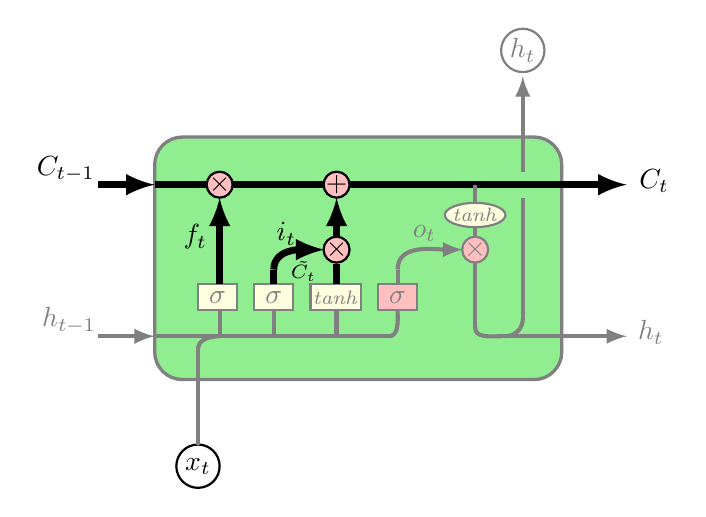
\begin{tikzpicture}[scale=1.1]

  % The grid
  % \draw[step=0.5, gray!40, very thin] (0,0) grid (8,4);

  % LSTM frame
  \def \yONE {0.5}
  \def \yTWO {3.3}
  \draw[rounded corners=10pt, very thick, gray,fill=LightGreen]  (1.5, 0.5) rectangle (6.2, 3.3);

  \def \sigmoidWidth  {0.45}
  \def \sigmoidInDist {0.2}
  \def \sigmoidHeight  {0.3}
  \def \yB  {1.3}
  \def \yD  {2.75}
  \def \shift {0.3}
  % First Sigmoid
  \draw[thick,gray,fill=LightYellow] (2, \yB) rectangle (2+ \sigmoidWidth, \yB + \sigmoidHeight) node[pos=0.5] {$\sigma$};

  \def \r {.15cm}
  % The Upper times operator % first time from left
  \draw[thick,fill=pink] (2.25, \yD) circle (\r) node {$\times$};

  % Second Sigmoid
  \def \xS {2.45 +\sigmoidInDist}
  \draw[thick,gray,fill=LightYellow]  (\xS, \yB) rectangle (\xS +\sigmoidWidth, \yB + \sigmoidHeight) node[pos=0.5] {$\sigma$};

  % Square tanh
  \def \xSS {\xS +\sigmoidWidth + \sigmoidInDist}
  \draw[thick,gray,fill=LightYellow]  (\xSS, \yB) 
  rectangle 
  (\xSS +\sigmoidWidth +0.13, \yB +\sigmoidHeight)
  node[pos=0.5] {\scriptsize \textit{tanh}};

  % Third Sigoid
  \def \xSSS {\xSS +\sigmoidWidth +0.13 +\sigmoidInDist}
  \draw[thick,gray,fill=pink]  (\xSSS, \yB) rectangle (\xSSS +\sigmoidWidth, \yB +\sigmoidHeight)
  node[pos=0.5] { $\sigma$};

  % Second times operator and add operator
  \def \xTimesB {3.6}
  \def \yC      {2}

  \draw[thick,fill=pink] (\xTimesB, \yC) circle (\r) node {$\times$};
  
  %%%%% **first line sectond operator +
  \draw[thick,fill=pink] (\xTimesB, \yD) circle (\r) node {$+$};

  % Third times operator and its tanh
  \draw[thick,gray,fill=pink] (\xTimesB +1.3 +\shift, \yC) circle (\r) node {$\times$};
  \draw[thick,gray,fill=LightYellow] (\xTimesB +1.3 +\shift, \yC +.4)  
  ellipse (.35cm and .14cm) 
  node {\scriptsize \textit{tanh}};


  % LINES %%% Upper line from c_{t -1} till C_t
  \draw[arrows=-latex, line width=2.5pt]  (0.85, \yD) -- (1.5, \yD) node[left, xshift=-.6cm, yshift=0.2cm] {$C_{t-1}$};
  \draw[line width=2.5pt]  (1.5, \yD) -- (2.1, \yD);
  \draw[line width=2.5pt]  (2.4, \yD) -- (3.46, \yD);
  \draw[arrows=-latex, line width=2.5pt]  (3.75, \yD) -- (6.75 +0.2, \yD)
  node[right, xshift=0.0cm, yshift=0.05cm] {$C_t$};

  %%%%first line from left from sigmoid ft till times input from C_{t-1}
  \draw[arrows=-latex, line width=2.5pt]  (2.25, \yB +\sigmoidHeight) -- (2.25, 2.6)
  node[left, yshift=-0.5cm] {$f_t$};

  % Level B LINES
  \def \levelB {1}
  %input h_{t-1} line
  \draw[arrows=-latex, line width=1.5pt,gray] (0.85, \levelB) -- (1.5, \levelB)
  node[left, xshift=-.6cm, yshift=0.2cm] {$h_{t-1}$};

%level B line base between input h_{t-1} and first sigmoid
  \draw[line width=1.5pt,gray] (1.5, \levelB) 
  --
  (2.25, \levelB);
  
  %level B line base between  first sigmoid and tanh
   \draw[line width=1.5pt,gray] (2.25, \levelB) 
  --
  (3.6, \levelB);
  
  %level B line base between  tanh and tanh angle
  \draw[line width=1.5pt,gray] (3.6, \levelB) 
  --
  (4.2, \levelB);

  \def \xOfThirdSigmoid {\xSSS + \sigmoidWidth/2}
  %second line last angle connected to sigmoid 
  \draw[line width=1.5pt,gray] (4.2, \levelB) to[out=0,in=270] (\xOfThirdSigmoid, \yB);

  % Third Sigmoid up line
  % END (\xTimesB +1.3 - 0.19 , \yC)
  \draw[line width=1.5pt,gray] (\xOfThirdSigmoid, \yB + \sigmoidHeight) 
  --
  (\xOfThirdSigmoid, \yB + \sigmoidHeight + 0.17) ;

  \draw[arrows=-latex, line width=1.5pt,gray] (\xOfThirdSigmoid, \yB + \sigmoidHeight+0.17) 
  to[out=90, in=180] 
  (\xTimesB +1.3 -0.14 +\shift , \yC) 
  node [left, yshift=0.2cm, xshift=-0.2cm] {$o_t$};

  % tanh line
  \draw [line width=1.5pt,gray] (\xTimesB, \levelB)
  --
  (\xTimesB, \yB);

%line between first tanh from left and x %%%%
  \draw [line width=2.5pt] (\xTimesB, \yB + \sigmoidHeight)
  --
  (\xTimesB, \yB + \sigmoidHeight +0.24)
  node [left, yshift=-0.1cm, xshift=-0.1cm] {\scriptsize$\tilde{C_t}$};

%line between x and + upper first tanh from left
  \draw [arrows=-latex, line width=2.5pt] (\xTimesB, 2.15)
  --
  (\xTimesB, 2.6);

%line between level B and first sigmoid
  \draw[line width=1.5pt,gray] (2.25, \levelB)
  --
  (2.25, \yB);
  
  % line between level B and second sigmoid
  \draw[line width=1.5pt,gray] (\xS +\sigmoidWidth/2, \levelB)
  --
  (\xS +\sigmoidWidth/2, \yB);

% line angle between sgima and x midlle line
  \draw[line width=2.5pt] (\xS +\sigmoidWidth/2, \yB +\sigmoidHeight)
  -- 
  (\xS +\sigmoidWidth/2, \yB +\sigmoidHeight + 0.17);

  %% angle between sgima and x midlle line i_t
  \draw[arrows=-latex, line width=2.5pt] (\xS +\sigmoidWidth/2, \yB + \sigmoidHeight+0.17) 
  to[out=90, in=180] 
  (\xTimesB-0.14, \yC)
  node [left, yshift=0.2cm, xshift=-0.2cm] {$i_t$};

  \def \bigR {0.25cm}
  \def \C    {1}
  \def \xBigCicleONE {2}
  \def \xBigCicleTWO {5.5 + 0.25}
  \draw[thick] (\xBigCicleONE, \yONE - \C) circle (\bigR) node {$x_t$};
  \draw[thick,gray] (\xBigCicleTWO, \yTWO + \C) circle (\bigR) node {$h_t$};

  % LINE Circle ONE from xt to line B
  \draw[line width=1.5pt,gray] (\xBigCicleONE, \yONE -\C +0.25) 
  --
  (\xBigCicleONE, \yONE -\C +0.25 + 1.1);

%% angle from the x_t to sigma ifrst angle from the left down
  \draw[line width=1.5pt,gray] (\xBigCicleONE, \yONE -\C +0.25 + 1.1)
  to[out=90, in=180]
  (2.25, 1);

  % LINE third \times betweem line B and times circle 
  \draw[line width=1.5pt,gray] (\xTimesB +1.3 +\shift, 1.1)
  --
  (\xTimesB +1.3 +\shift, \yC - 0.15);

  \draw[arrows=-latex, line width=1.5pt,gray] (5.5, 1) 
  --
  (6.75 +0.2, 1)
  node[right, xshift=0.0cm, yshift=0.05cm,] {$h_t$};

%%% second line last angle connect the input with h_t output
  \draw[line width=1.5pt,gray] (\xTimesB +1.3 +\shift, 1.1)
  to[out=270, in=180]
  (5.5, 1);


%%% line between times and tanh (last tanh h on the right alone)
  \draw[line width=1.5pt,gray] (\xTimesB +1.3 +\shift, 2.14)
  --
  (\xTimesB +1.3 +\shift, 2.26);

%%%%% Line between tanh and Line level A 
  \draw[line width=1.5pt,gray] (\xTimesB +1.3 +\shift, \yD)
  --
  (\xTimesB +1.3 +\shift, 2.54);

%%%%% first horizontal line from the right angle connected to the line which connect to output ht
  \draw[line width=1.5pt,gray] (\xBigCicleTWO, \levelB +0.2)
  --
  (\xBigCicleTWO, 2.6);

%%%%% first horizontal line from the right angle connected to output ht
  \draw[line width=1.5pt,gray] (\xBigCicleTWO - 0.2, \levelB)
  to[out=0, in=270]
  (\xBigCicleTWO, \levelB +0.2);

%%%%% first horizontal line from the right angle connected to output ht

  \draw[arrows=-latex, line width=1.5pt,gray]
  (\xBigCicleTWO, \yD +0.15)
  --
  (\xBigCicleTWO, 4);
  
\end{tikzpicture}

	}
	\subfigure[LSTM output gate.]
	{
		\label{Fig:LSTM_Output_Gate}
		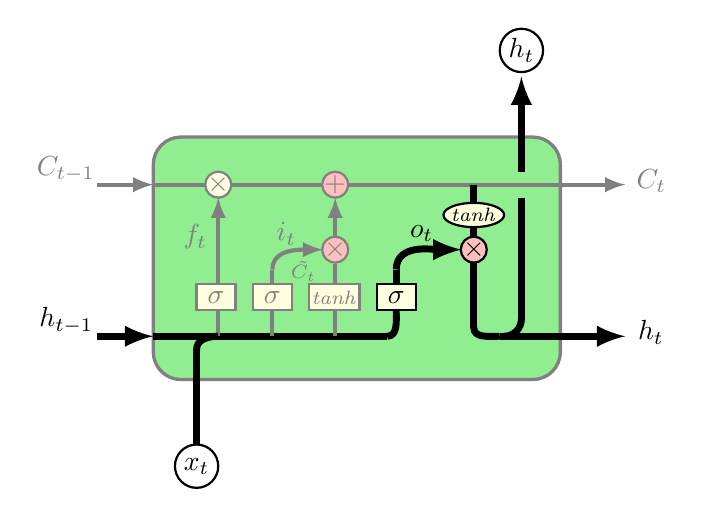
\begin{tikzpicture}[scale=1.1]

  % The grid
  % \draw[step=0.5, gray!40, very thin] (0,0) grid (8,4);

  % LSTM frame
  \def \yONE {0.5}
  \def \yTWO {3.3}
  \draw[rounded corners=10pt, very thick, gray,fill=LightGreen]  (1.5, 0.5) rectangle (6.2, 3.3);

  \def \sigmoidWidth  {0.45}
  \def \sigmoidInDist {0.2}
  \def \sigmoidHeight  {0.3}
  \def \yB  {1.3}
  \def \yD  {2.75}
  \def \shift {0.3}
  % First Sigmoid
  \draw[thick,gray,fill=LightYellow] (2, \yB) rectangle (2+ \sigmoidWidth, \yB + \sigmoidHeight) node[pos=0.5] {$\sigma$};

  \def \r {.15cm}
  % The Upper times operator % first time from left
  \draw[thick,gray,fill=LightYellow] (2.25, \yD) circle (\r) node {$\times$};

  % Second Sigmoid
  \def \xS {2.45 +\sigmoidInDist}
  \draw[thick,gray,fill=LightYellow]  (\xS, \yB) rectangle (\xS +\sigmoidWidth, \yB + \sigmoidHeight) node[pos=0.5] {$\sigma$};

  % Square tanh
  \def \xSS {\xS +\sigmoidWidth + \sigmoidInDist}
  \draw[thick,gray,fill=LightYellow]  (\xSS, \yB) 
  rectangle 
  (\xSS +\sigmoidWidth +0.13, \yB +\sigmoidHeight)
  node[pos=0.5] {\scriptsize \textit{tanh}};

  % Third Sigoid
  \def \xSSS {\xSS +\sigmoidWidth +0.13 +\sigmoidInDist}
  \draw[thick,fill=LightYellow]  (\xSSS, \yB) rectangle (\xSSS +\sigmoidWidth, \yB +\sigmoidHeight)
  node[pos=0.5] { $\sigma$};

  % Second times operator and add operator
  \def \xTimesB {3.6}
  \def \yC      {2}

  \draw[thick,gray,fill=pink] (\xTimesB, \yC) circle (\r) node {$\times$};
  
  %%%%% **first line sectond operator +
  \draw[thick,gray,fill=pink] (\xTimesB, \yD) circle (\r) node {$+$};

  % Third times operator 
  \draw[thick,fill=pink] (\xTimesB +1.3 +\shift, \yC) circle (\r) node {$\times$};
  
  %second tanh 
  \draw[thick,fill=LightYellow] (\xTimesB +1.3 +\shift, \yC +.4)  
  ellipse (.35cm and .14cm) 
  node {\scriptsize \textit{tanh}};


  % LINES %%% Upper line from c_{t -1} till C_t
  \draw[arrows=-latex, line width=1.5pt,gray]  (0.85, \yD) -- (1.5, \yD) node[left, xshift=-.6cm, yshift=0.2cm] {$C_{t-1}$};
  \draw[line width=1.5pt,gray]  (1.5, \yD) -- (2.1, \yD);
  \draw[line width=1.5pt,gray]  (2.4, \yD) -- (3.46, \yD);
  \draw[arrows=-latex, line width=1.5pt,gray]  (3.75, \yD) -- (6.75 +0.2, \yD)
  node[right, xshift=0.0cm, yshift=0.05cm] {$C_t$};

  %%%%first line from left from sigmoid ft till times input from C_{t-1}
  \draw[arrows=-latex, line width=1.5pt,gray]  (2.25, \yB +\sigmoidHeight) -- (2.25, 2.6)
  node[left, yshift=-0.5cm] {$f_t$};

  % Level B LINES
  \def \levelB {1}
  %input h_{t-1} line
  \draw[arrows=-latex, line width=2.5pt] (0.85, \levelB) -- (1.5, \levelB)
  node[left, xshift=-.6cm, yshift=0.2cm] {$h_{t-1}$};

%level B line base between input h_{t-1} and first sigmoid
  \draw[line width=2.5pt] (1.5, \levelB) 
  --
  (2.25, \levelB);
  
  %level B line base between  first sigmoid and tanh
   \draw[line width=2.5pt] (2.25, \levelB) 
  --
  (3.6, \levelB);
  
  %level B line base between  tanh and tanh angle
  \draw[line width=2.5pt] (3.6, \levelB) 
  --
  (4.2, \levelB);

  \def \xOfThirdSigmoid {\xSSS + \sigmoidWidth/2}
  %second line last angle connected to sigmoid 
  \draw[line width=2.5pt] (4.2, \levelB) to[out=0,in=270] (\xOfThirdSigmoid, \yB);

  % Third Sigmoid up line
  % END (\xTimesB +1.3 - 0.19 , \yC)
  \draw[line width=2.5pt] (\xOfThirdSigmoid, \yB + \sigmoidHeight) 
  --
  (\xOfThirdSigmoid, \yB + \sigmoidHeight + 0.17) ;

  \draw[arrows=-latex, line width=2.5pt] (\xOfThirdSigmoid, \yB + \sigmoidHeight+0.17) 
  to[out=90, in=180] 
  (\xTimesB +1.3 -0.14 +\shift , \yC) 
  node [left, yshift=0.2cm, xshift=-0.2cm] {$o_t$};

  % tanh line from line B to third tirangle tanh
  \draw [line width=1.5pt,gray] (\xTimesB, \levelB)
  --
  (\xTimesB, \yB);

%line between first tanh from left and x %%%%
  \draw [line width=1.5pt,gray] (\xTimesB, \yB + \sigmoidHeight)
  --
  (\xTimesB, \yB + \sigmoidHeight +0.24)
  node [left, yshift=-0.1cm, xshift=-0.1cm] {\scriptsize$\tilde{C_t}$};

%line between x and + upper first tanh from left
  \draw [arrows=-latex, line width=1.5pt,gray] (\xTimesB, 2.15)
  --
  (\xTimesB, 2.6);

%line between level B and first sigmoid
  \draw[line width=1.5pt,gray] (2.25, \levelB)
  --
  (2.25, \yB);
  
  % line between level B and second sigmoid
  \draw[line width=1.5pt,gray] (\xS +\sigmoidWidth/2, \levelB)
  --
  (\xS +\sigmoidWidth/2, \yB);

% line angle between sgima and x midlle line
  \draw[line width=1.5pt,gray] (\xS +\sigmoidWidth/2, \yB +\sigmoidHeight)
  -- 
  (\xS +\sigmoidWidth/2, \yB +\sigmoidHeight + 0.17);

  %% angle between sgima and x midlle line i_t
  \draw[arrows=-latex, line width=1.5pt,gray] (\xS +\sigmoidWidth/2, \yB + \sigmoidHeight+0.17) 
  to[out=90, in=180] 
  (\xTimesB-0.14, \yC)
  node [left, yshift=0.2cm, xshift=-0.2cm] {$i_t$};

  \def \bigR {0.25cm}
  \def \C    {1}
  \def \xBigCicleONE {2}
  \def \xBigCicleTWO {5.5 + 0.25}
  \draw[thick] (\xBigCicleONE, \yONE - \C) circle (\bigR) node {$x_t$};
  \draw[thick] (\xBigCicleTWO, \yTWO + \C) circle (\bigR) node {$h_t$};

  % LINE Circle ONE from xt to line B
  \draw[line width=2.5pt] (\xBigCicleONE, \yONE -\C +0.25) 
  --
  (\xBigCicleONE, \yONE -\C +0.25 + 1.1);

%% angle from the x_t to sigma ifrst angle from the left down
  \draw[line width=2.5pt] (\xBigCicleONE, \yONE -\C +0.25 + 1.1)
  to[out=90, in=180]
  (2.25, 1);

  % LINE third \times betweem line B and times circle 
  \draw[line width=2.5pt] (\xTimesB +1.3 +\shift, 1.1)
  --
  (\xTimesB +1.3 +\shift, \yC - 0.15);

  \draw[arrows=-latex, line width=2.5pt] (5.5, 1) 
  --
  (6.75 +0.2, 1)
  node[right, xshift=0.0cm, yshift=0.05cm,] {$h_t$};

%%% second line last angle connect the input with h_t output
  \draw[line width=2.5pt] (\xTimesB +1.3 +\shift, 1.1)
  to[out=270, in=180]
  (5.5, 1);


%%% line between times and tanh (last tanh h on the right alone)
  \draw[line width=2.5pt] (\xTimesB +1.3 +\shift, 2.14)
  --
  (\xTimesB +1.3 +\shift, 2.26);

%%%%% Line between tanh and Line level A 
  \draw[line width=2.5pt] (\xTimesB +1.3 +\shift, \yD)
  --
  (\xTimesB +1.3 +\shift, 2.54);

%%%%% first horizontal line from the right angle connected to the line which connect to output ht
  \draw[line width=2.5pt] (\xBigCicleTWO, \levelB +0.2)
  --
  (\xBigCicleTWO, 2.6);

%%%%% first horizontal line from the right angle connected to output ht
  \draw[line width=2.5pt] (\xBigCicleTWO - 0.2, \levelB)
  to[out=0, in=270]
  (\xBigCicleTWO, \levelB +0.2);

%%%%% first horizontal line from the right angle connected to output ht

  \draw[arrows=-latex, line width=2.5pt]
  (\xBigCicleTWO, \yD +0.15)
  --
  (\xBigCicleTWO, 4);
  
\end{tikzpicture}

	}
	\subfigure[GRU cell architecture.]
	{
		\label{Fig:GRU}
		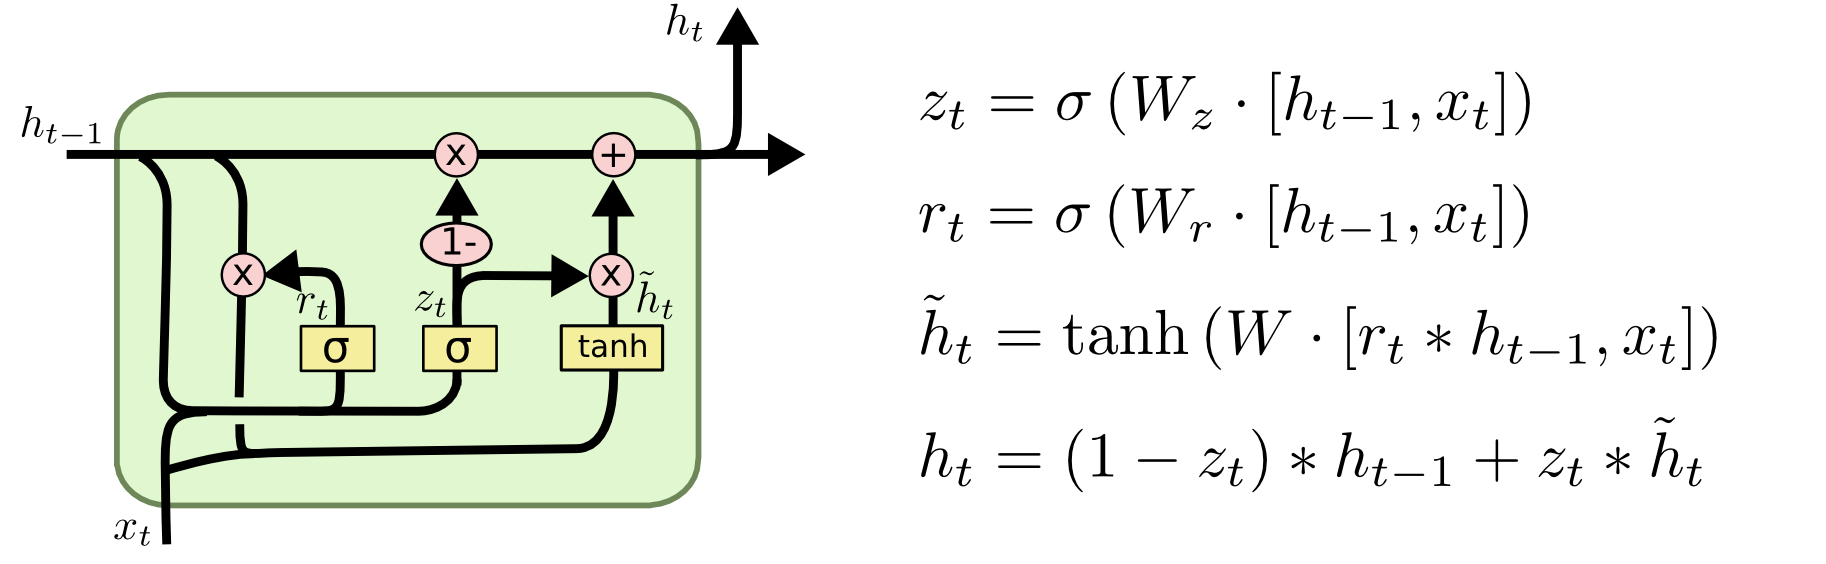
\includegraphics[scale=0.6]{./Figures/Ch_2_Background/GRU.png}
	}
	\caption{LSTM Gates and Configurations adapted from~\cite{colah}}
\end{figure}%

\subsubsection{BI-LSTM}\label{Sec:Bi_Lstm}

BI-LSTM refers to two LSTMs stacked on top of each other used to solve some problem where the information needs to be considered in both directions for LSTM. As the normal LSTM is working from left to right, the BI-LSTM adds the other directions into the learning information. Consider a motivation example regarding why we need BI-LSTM:

\begin{itemize}
\item \textit{Harry is the king, and he will travel next week.}
\item \textit{The new book which makes the big sale is named Harry Potter.}.
\end{itemize}

Harry in the first example refers to a person, but in the second example refers to a book. So, if we are working left to right, we do not get the type of word Harry represents in the second example.

The architecture in BI-LSTM is similar to what we discussed previously regarding Uni-LSTM. We can mention here that BI-LSTM is very slow compared to LSTM, and needs much time in the training phase but, as we see later in our research, it is impressive regarding the results and the effect on the language problems.

Figure~\ref{Fig:BI-LSTM} represents a recurrent neural network consisting of several LSTM blocks, processing the input sequence simultaneously forwards and backwards (to exploit both directions of temporal dependence). In Figure~\ref{Fig:LSTM_CharLevel} we can observe a similar example to our encoding data, which feeds the networks using a sequence of char, then passes to the BI-LSTM cells, then produces the character representations to feed the next layer of the network. Figure~\ref{Fig:LSTM_Arch} shows the simple example of the full network from char-level embedding (encoding) till the last sequence which outputs to softmax layer.%
\begin{figure}[!t]
 \centering
 \subfigure[bidirectional long short-term memory~\cite{Gitrepo_NN_Tikz}]
 {
  \label{Fig:BI-LSTM}
  \begin{tikzpicture}
	\node[rectangle] (Y0) at (0, 0) {$\dots$};
	\node[rectangle, draw, right=2em of Y0, minimum height=1cm, minimum width=1cm] (RNN) {LSTM$_\rightarrow$};
	\node[rectangle, right=of RNN, draw, minimum height=1cm, minimum width=1cm] (RNN2) {LSTM$_\rightarrow$};
	\node[rectangle, right=of RNN2, draw, minimum height=1cm, minimum width=1cm] (RNN3) {LSTM$_\rightarrow$};
			
	\node[rectangle, right= of RNN3, draw, minimum height=1cm, minimum width=1cm] (RNN4) {LSTM$_\rightarrow$};
	\node[rectangle, right=2em of RNN4] (RNN5) {$\dots$};
			
			
	\node[rectangle, above=of RNN4, draw, minimum height=1cm, minimum width=1cm] (R25) {LSTM$_\leftarrow$};
	\node[rectangle, left=of R25, minimum height=1cm, minimum width=1cm, draw] (R24) {LSTM$_\leftarrow$};
	\node[rectangle, left=of R24, draw, minimum height=1cm, minimum width=1cm] (R23) {LSTM$_\leftarrow$};
	\node[rectangle, left=of R23, draw, minimum height=1cm, minimum width=1cm] (R22) {LSTM$_\leftarrow$};
	\node[rectangle, left=2em of R22] (R21) {$\dots$};
	\node[right=2em of R25] (Y20) {$\dots$};
			
	\node[below=of RNN] (X1) {$\vec{x}_2$};
	\node[below=of RNN2] (X2) {$\vec{x}_3$};
	\node[below=of RNN3] (X3) {$\vec{x}_4$};
	\node[below=of RNN4] (X4) {$\vec{x}_5$};
	\node[above=of R25] (Y5) {$\vec{h}_5$};
	\node[above=of R24] (Y4) {$\vec{h}_4$};
	\node[above=of R23] (Y3) {$\vec{h}_3$};
	\node[above=of R22] (Y2) {$\vec{h}_2$};
			
	\draw[-stealth, thick] (X1) -- (RNN);
	\draw[-stealth, thick] (X2) -- (RNN2);
	\draw[-stealth, thick] (X3) -- (RNN3);
	\draw[-stealth, thick] (X4) -- (RNN4);
	\draw[-stealth, thick, densely dotted] (Y0) -- (RNN);
	\draw[-stealth, thick] (RNN) -- node[above, pos=0.35] {$\vec{h}_2^\rightarrow$} (RNN2);
	\draw[-stealth, thick] (RNN2) -- node[above, pos=0.35] {$\vec{h}_3^\rightarrow$} (RNN3);
	\draw[-stealth, thick] (RNN3) -- node[above, pos=0.35] {$\vec{h}_4^\rightarrow$} (RNN4);
	\draw[-stealth, densely dotted, thick] (RNN4) -- (RNN5);
	\node[below=4em of Y0] (d) {\dots};
	\node[below=4em of RNN5] (d) {\dots};
			
	\path[-stealth, ultra thick, white] (X1) edge[bend left=45] (R22);
	\path[-stealth, thick] (X1) edge[bend left=45] (R22);
	\path[-stealth, ultra thick, white] (X2) edge[bend left=45] (R23);
	\path[-stealth, thick] (X2) edge[bend left=45] (R23);
	\path[-stealth, ultra thick, white] (X3) edge[bend left=45] (R24);
	\path[-stealth, thick] (X3) edge[bend left=45] (R24);
	\path[-stealth, ultra thick, white] (X4) edge[bend left=45] (R25);
	\path[-stealth, thick] (X4) edge[bend left=45] (R25);
	\draw[-stealth, densely dotted, thick] (Y20) -- (R25);
			
	\draw[-stealth, thick] (R22) -- (Y2);
	\draw[-stealth, thick] (R23) -- (Y3);
	\draw[-stealth, thick] (R24) -- (Y4);
	\draw[-stealth, thick] (R25) -- (Y5);
		
	\draw[stealth-, densely dotted, thick] (R21) -- (R22);
	\draw[stealth-, thick] (R22) -- node[above, pos=0.65] {$\vec{h}_3^\leftarrow$} (R23);
	\draw[stealth-, thick] (R23) -- node[above, pos=0.65] {$\vec{h}_4^\leftarrow$} (R24);
	\draw[stealth-, thick] (R24) -- node[above, pos=0.65] {$\vec{h}_5^\leftarrow$} (R25);
	\draw[-stealth, densely dotted, thick] (Y20) -- (R25);	
			
	\path[-stealth, ultra thick, white] (RNN) edge[bend right=45] (Y2);
	\path[-stealth, thick] (RNN) edge[bend right=45] (Y2);
	\path[-stealth, ultra thick, white] (RNN2) edge[bend right=45] (Y3);
	\path[-stealth, thick] (RNN2) edge[bend right=45] (Y3);
	\path[-stealth, ultra thick, white] (RNN3) edge[bend right=45] (Y4);
	\path[-stealth, thick] (RNN3) edge[bend right=45] (Y4);
	\path[-stealth, ultra thick, white] (RNN4) edge[bend right=45] (Y5);
	\path[-stealth, thick] (RNN4) edge[bend right=45] (Y5);
			
\end{tikzpicture}

 }
 \subfigure[character-based representation using BiLSTM~\cite{ReimersG17}]
 {
 \label{Fig:LSTM_CharLevel}
  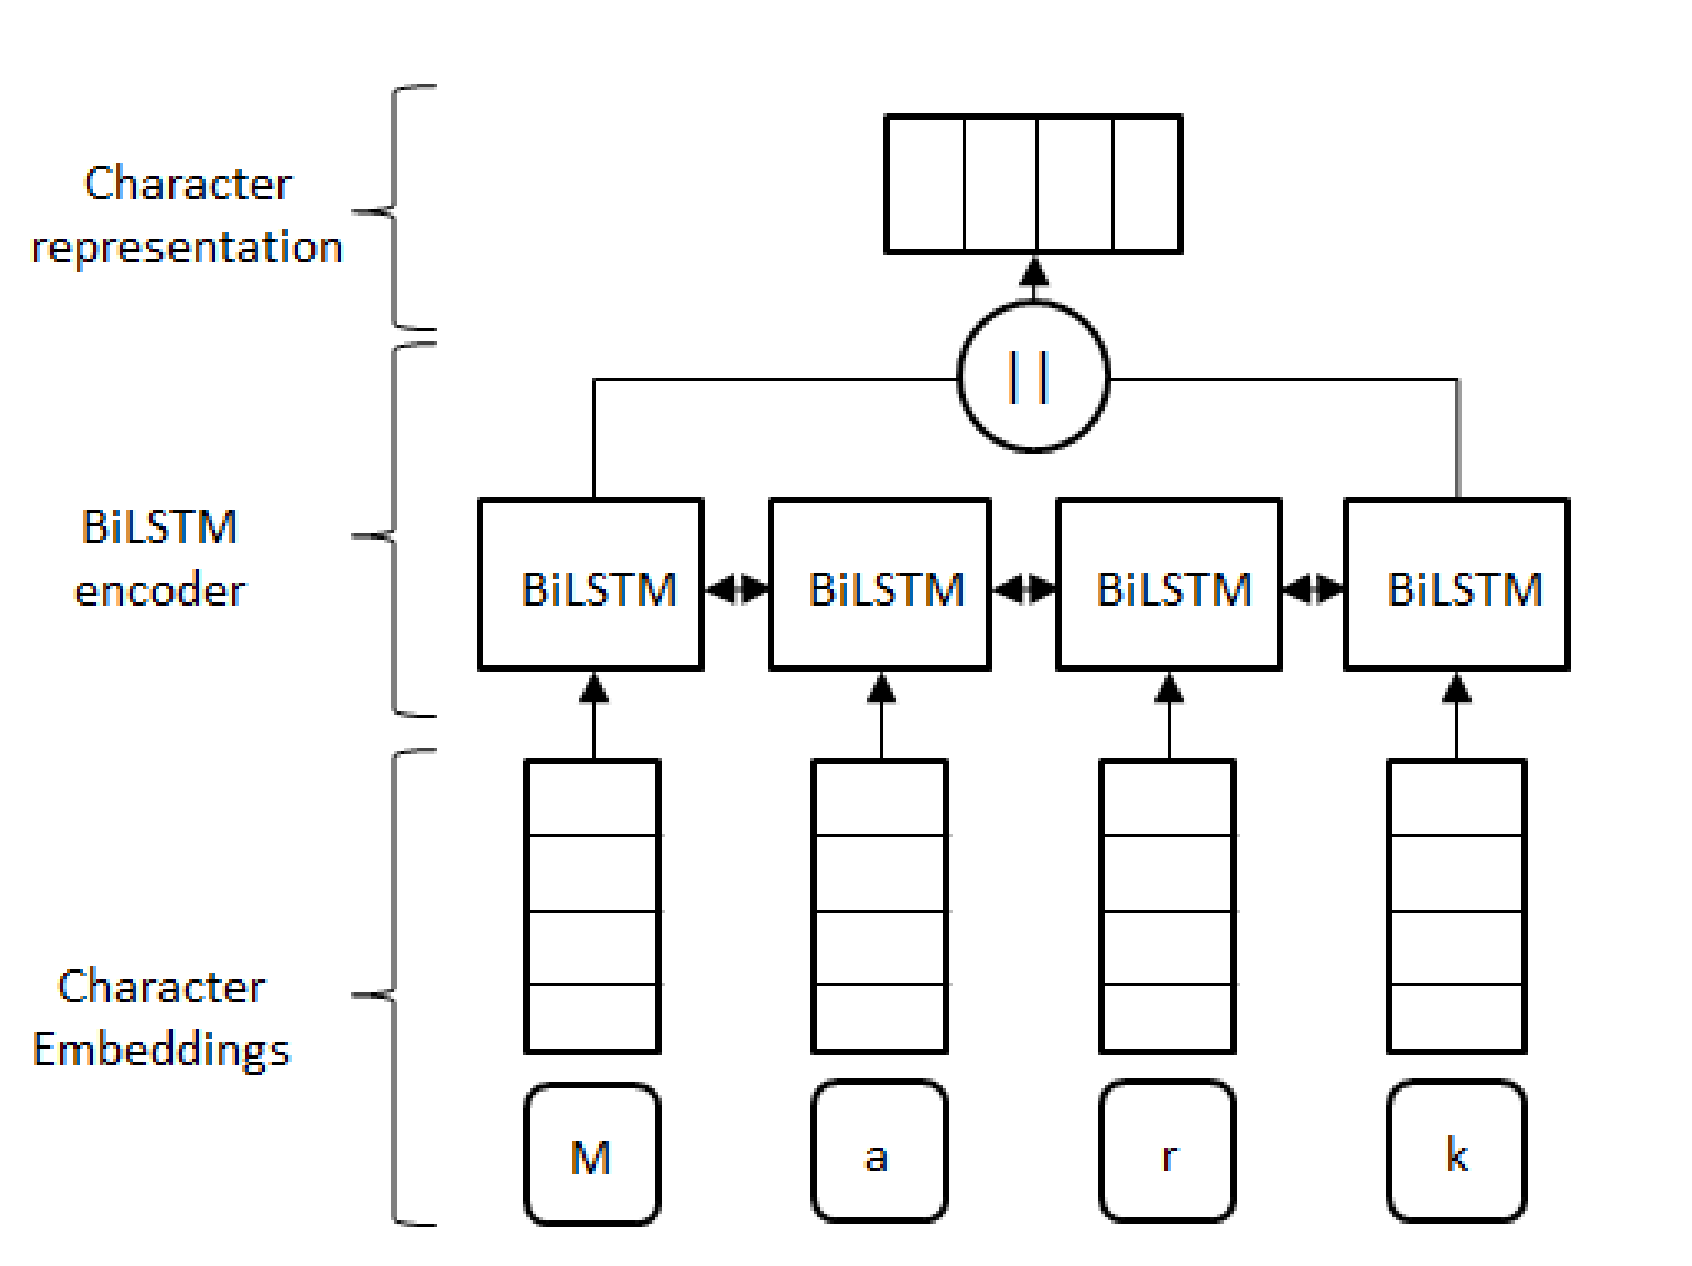
\includegraphics[width=8cm,height=7cm]{./Figures/Ch_2_Background/BI_LSTM_2.png}

 }
 \subfigure[An example of the architecture of LSTM~\cite{Blog_LSTM}]
 { 
  \label{Fig:LSTM_Arch}
  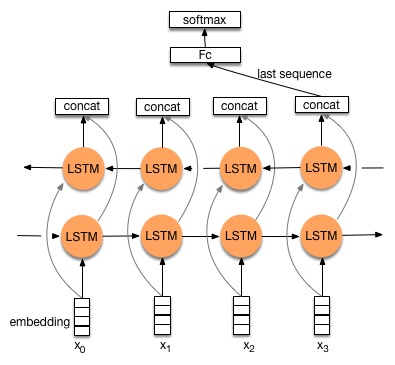
\includegraphics[width=8cm,height=7cm]{./Figures/Ch_2_Background/BI_LSTM_1.jpg}
 }
%\caption{LSTM Gates and Configurations adapopted from~\cite{colah}.}
\end{figure}%


\subsection{Machine Learning Model Assessment}

As explained previously, machine learning cycle starts by Data preparation, Feature extraction, Model training and Model assessment~\ref{Fig:Thesis_Cycle}. In this section we explain the meaning by model assessment. we also discuss different techniques for model assessment.

In Supervised machine learning problems, we have two types \textit{Classification and Regression}. Classification of the output is discrete variables, for example, Spam vs Normal Email detection. In Regression, the output is a continuous variable: for example, Predict Housing Price. Each type of problem has its methods or performance evaluation matrix. In this section, we focus on Classification problem, as our problem is a meter classifier application.

How can we measure the model performance? It is good when the difference between the predicted value and the actual is small and not overfitting on the development dataset.

There are many ways to measure classification performance. Before we explain every method, we give a simple example to allow us to understand the output of every method. Let us assume we have a binary classifier which detects Spam vs Normal Emails. we explain by example the definition for every type base on the example data in Table~\ref{Tab:EmailClassifier}%
\begin{table}[t]
 \centering
 \begin{tabular}{c c c c}
  \toprule
  \textbf{Label}& \textbf{Actual Number}& \textbf{Actual Spam (Positive)} & \textbf{Actual Normal (Negative)}\\
  \midrule
  Predicted as Spam (Positive)  & 200 & \cellcolor{green!25}160 & \cellcolor{red!25}40 \\
  Predicted as Normal (Negative)   & 300  & \cellcolor{red!25}10  & \cellcolor{green!25}290\\
  \bottomrule
 \end{tabular}
 \caption{Spam vs Normal Email Classifier example}\label{Tab:EmailClassifier}
\end{table}%
%
\subsubsection{Accuracy}

Accuracy measures the corrected prediction over the dataset. It is calculated using the ratio between the corrected predicted sample from the test data over the total test data sample. Ex: in Table~\ref{Tab:EmailClassifier}\textit{(the total positive predicted as positive + the total negative predicted as negative)/total number of test data}~\eqref{eq:accuracy_calculation} which means 90\%. An issue in Accuracy as a measurement is that it doesn’t give us any sense of the results with respect to the actual performance of the positive, calculated as positive and vice-versa. One measurement which gives us some sense is the Precision and Recall, which we discuss it in the next section.%
\begin{equation}\label{eq:accuracy_calculation}
\frac{\text{the total positive predicted as positive + the total negative predicted as negative}}{\text{total number of test data}} = \frac{160+290}{500}=0.9 
\end{equation}%


\subsubsection{Precision and Recall}

Precision and Recall are two measurements which answer questions related to our model performance. Some applications consider one of them and others require both or a combination. Before explaining it, we should prepare a data table named Confusion Matrix similar to the example in~\ref{Tab:EmailClassifier}.

\begin{itemize}
\item Precision (also called positive predictive value) is used to answer the question, \textbf{Based on the test data how many items predicted correctly from the test data sample}. It can be calculated from Equation~\eqref{eq:precision}.
\item Recall (also known as sensitivity) answers another question: \textbf{Based on the test data, how many of the truly predicted items are truly predicted}. We can calculate this using Equation~\eqref{eq:recall}.
\end{itemize}
\begin{equation}\label{eq:precision}
precision = \frac{\text{true positives}}{\text{true positives + false positives}} = \frac{160}{160 + 40}=0.8
\end{equation}%


\begin{equation}\label{eq:recall}
recall = \frac{\text{true positives}}{\text{true positives + false negatives}} = \frac{160}{160 + 10}=0.941
\end{equation}%

We need to highlight that some applications could require a focus on precision more than recall and vice-versa. We therefore need to choose the right measure based on our problem.
 
\subsubsection{$F_1$ Score}
In statistical analysis of binary classification, the F1 score is a measure of a test's accuracy. It considers both the precision \textit{p} and the recall \textit{r} of the test to compute the accuracy score. The F1 score is the harmonic average of the precision and recall, where an F1 score reaches its best value at 1 (perfect precision and recall) and worst at 0~\cite{Wiki_f1_score}. We can calculate it using Equation~\eqref{eq:f_1}.%
\begin{equation}\label{eq:f_1}
F_1= 2 \times \frac{precision*recall}{precision+recall}
\end{equation}%
 
\subsubsection{Per-Class Accuracy}

Per class, accuracy is one of the important accuracy measures when we have multi-class. There is a difference between each accuracy calculation regarding the dataset classes distribution. Most of the performance measurement calculate the average accuracy per-class but the difference is some of them take into consideration the size of each class and some don’t take the size. So, in case we have imbalanced dataset we should use the type which considers the class size for the accuracy of calculations. In case the data is imbalanced the results could hide information about how the model is performing. For example, assuming the model working perfectly with a class which has the most amount of our data and performing badly in the other class the accuracy can give us high results. However, if we use the average per-class, it will give us a more clear vision of how the model is performing regarding the dataset size for each class. Below is common types used in most of the framework to calculate accuracy per-class. Note: The below naming is followed the same as \textit{Sklearn} Library.

\begin{itemize}
 \item Weighted: Calculates the F1 score for each class independently but when it adds them together uses a weight that depends on the number of true labels of each class~\eqref{eq:f_1_weighted}.%
\begin{equation}\label{eq:f_1_weighted}
F_{1 class1}\times W_1 + F_{2 class2}\times W_2 + F_{3 class3}\times W_3
\end{equation}%

 \item Micro: Uses the global number of TP, FN, FP and calculates the F1 directly~\eqref{eq:f_1_micro}. It does not take into consideration the size for each class.%
 \begin{equation}\label{eq:f_1_micro}
F_{1 class1+class2+class3}
\end{equation}%
 \item Macro: Calculates the F1 separated by class but not using weights for the aggregation~\eqref{eq:f_1_macro}  which results in a bigger penalization when the model does not perform well with the minority classes.%
\begin{equation}\label{eq:f_1_macro}
F_{1 class1} + F_{2 class2} + F_{3 class3}
\end{equation}%
\end{itemize}

%%% Local Variables:
%%% mode: latex
%%% TeX-master: "../master"
%%% TeX-engine: xetex
%%% End: